\documentclass[sigconf]{acmart}
\newcommand{\DIFdelFL}[1]{}
\newcommand{\DIFaddFL}[1]{}

%DIF LATEXDIFF DIFFERENCE FILE
%DIF DEL ../hotpot-original-with-acm/paper.tex   Wed Aug  9 06:20:56 2017
%DIF ADD paper.tex                               Wed Aug  9 06:20:56 2017

\usepackage{booktabs}
\usepackage{setspace}
\usepackage{listings}
\usepackage{courier}
\usepackage{enumitem}
\usepackage{multirow}
\usepackage{color}
\usepackage{xcolor}

  \let\oldthebibliography=\thebibliography
  \let\endoldthebibliography=\endthebibliography
  \renewenvironment{thebibliography}[1]{%
    \begin{oldthebibliography}{#1}%
      \setlength{\parskip}{0ex}%
      \setlength{\itemsep}{0ex}%
  }%
  {%
    \end{oldthebibliography}%
  }


\sloppy

\newcommand{\mm}{mm$^2$}
\newcommand{\figtitle}[1]{\textbf{#1}}
\newcommand{\us}{$\mu$s}
\newcommand{\fixme}[1]{{\color{red}\textbf{#1}}}

\definecolor{pink}{rgb}{1.0,0.47,0.6}
\newcommand{\adrian}[1]{{\color{green}\textbf{#1}}}
\newcommand{\laura}[1]{{\color{pink}\textbf{#1}}}
\newcommand{\joel}[1]{{\color{red}\textbf{#1}}}
\newcommand{\ameen}[1]{{\color{blue}\textbf{#1}}}
\newcommand{\arup}[1]{{\color{yellow}\textbf{#1}}}
\newcommand{\hungwei}[1]{{\color{purple}\textbf{#1}}}


\newcommand{\note}[2]{\fixme{$\ll$ #1 $\gg$ #2}}

\newcommand{\myitem}[1]{\item \textbf{#1}}

%DIF 44a44-68
\lstloadlanguages{% Check Dokumentation for further languages ... %DIF > 
        %[Visual]Basic %DIF > 
        %Pascal %DIF > 
        C %DIF > 
        %C++ %DIF > 
        %XML %DIF > 
        %HTML %DIF > 
        %Java %DIF > 
} %DIF > 
 %DIF > 
\lstdefinestyle{customc}{ %DIF > 
  belowcaptionskip=1\baselineskip, %DIF > 
  breaklines=true, %DIF > 
  frame=b, %DIF > 
  xleftmargin=\parindent, %DIF > 
  language=C, %DIF > 
  showstringspaces=false, %DIF > 
  basicstyle=\scriptsize\ttfamily, %DIF > 
  keywordstyle=\bfseries\color{green!40!black}, %DIF > 
  commentstyle=\itshape\color{purple!40!black}, %DIF > 
  identifierstyle=\color{blue}, %DIF > 
  stringstyle=\color{red}, %DIF > 
} %DIF > 
\lstset{escapechar=@,style=customc} %DIF > 
 %DIF > 
%DIF -------
\newcommand{\horizbar}{\rule{\linewidth}{.5mm}}
\newcommand{\app}[1]{{\sc #1}}
 
\renewcommand{\em}{\it}

  
\newcommand{\BigO}[1]{${\cal O}(#1)$}
\newcommand{\BigOmega}[1]{$\Omega(#1)$}
\newcommand{\BigTheta}[1]{$\Theta(#1)$}
 
\newcommand{\ceiling}[1]{\left\lceil #1 \right\rceil}
\newcommand{\faM}{\lfloor \alpha M \rfloor}
%\newcommand{\C}[2]{{#1 \choose #2}}

\newcommand{\x}{$\times$}
 
%\newcommand{\comment}[1]{}
\newcommand{\ignore}[1]{}


%\newcommand{\boldparagraph}[1]{\vspace*{-0ex}\paragraph{#1}}
\newcommand{\boldparagraph}[1]{\vspace*{1ex}\noindent\textit{#1}\hspace{1em}}

%%%%% SINGLE FIGURE
\def\cfigure[#1,#2,#3]{
\begin{figure}
\vspace*{0mm}
\begin{center}

\includegraphics[width=3in]{#1} 
 
\vspace*{-3mm}\caption[]{#2
} \label{#3}
 
\vspace*{-5mm}
\end{center}
%\horizbar
%\vspace*{-2mm}
\end{figure}}

%%%%% SINGLE FIGURE 4in wide
\def\cfigurefour[#1,#2,#3]{
\begin{figure}
\vspace*{0mm}
\begin{center}

\includegraphics[width=4in]{#1} 
 
\vspace*{-3mm}\caption[]{#2
} \label{#3}
 
\vspace*{-5mm}
\end{center}
%\horizbar
%\vspace*{-2mm}
\end{figure}}

%%%%% SINGLE FIGURE
\def\cfiguretemp[#1,#2,#3]{
\begin{figure}
\vspace*{0mm}
\begin{center}

\includegraphics[width=3.5in]{#1} 
 
\vspace*{-3mm}\caption[]{#2
} \label{#3}
 
\vspace*{-5mm}
\end{center}
%\horizbar
\vspace*{-2mm}
\end{figure}}

%%%%% SINGLE WIDE FIGURE
\def\wfigure[#1,#2,#3]{
\begin{figure*}
\vspace*{0mm}
\begin{center}
 \includegraphics[width=\textwidth]{#1} 
 \vspace*{-3mm}\caption[]{#2
} \label{#3}
 
\end{center}
%\horizbar
\end{figure*}}

%%%%% 3 FIGURES IN A ROW
\def\threefigure[#1,#2,#3,#4,#5]{
\begin{figure*}
\vspace*{0mm}
\begin{center}

\begin{tabular}{ccc}
\includegraphics[width=2in]{#1} & \includegraphics[width=2in]{#2} &  \includegraphics[width=2in]{#3} \\
(a) & (b) & (c) \\
\end{tabular}

\vspace*{-3mm}\caption[]{#4
} \label{#5}

\vspace*{-5mm}
\end{center}
%\horizbar
\vspace*{-2mm}
\end{figure*}}

%%%%%% DOUBLE FIGURE
\def\dcfigure[#1,#2,#3,#4,#5,#6]{
{
\begin{figure*}
\begin{center}
\begin{minipage}[c]{\columnwidth}{
\includegraphics[width=\columnwidth]{#1} 
\vspace*{0mm}\caption[]{#2} \label{#3} \
}\end{minipage}\hspace*{\columnsep}\
\begin{minipage}[c]{\columnwidth}{
\includegraphics[width=\columnwidth]{#4} 
\vspace*{0mm}\caption[]{#5}\label{#6} \
}\end{minipage}
\end{center}
\end{figure*}
}
}


\def\tableByTable[#1,#2,#3,#4,#5,#6]{
{
\begin{table*}
\begin{center}
\begin{minipage}[c]{3in}{
\centering
{#1}
\vspace*{0mm}\tabcaption[]{#2}\label{#3} \
}\end{minipage}\hspace*{\columnsep}\
\begin{minipage}[c]{3in}{
\centering
{#4}
\vspace*{0mm}\tabcaption[]{#5}\label{#6} \
}\end{minipage}
\end{center}
\end{table*}
}
}


\def\figureByTable[#1,#2,#3,#4,#5,#6]{
{
\begin{figure*}
\begin{center}
\begin{minipage}[c]{3in}{
\centering
\includegraphics[width=\textwidth]{#1}
\vspace*{0mm}\figcaption[]{#2} \label{#3} \
}\end{minipage}\hspace*{\columnsep}\
\begin{minipage}[c]{3.3in}{
\centering
{#4}
\vspace*{0mm}\tabcaption[]{#5}\label{#6} \
}\end{minipage}
\end{center}
\end{figure*}
}
}

\def\tableByFigure[#1,#2,#3,#4,#5,#6]{
{
\begin{figure*}
\begin{center}
\begin{minipage}[c]{4.3in}{
\centering
{#1}
\vspace*{0mm}\tabcaption[]{#2} \label{#3} \
}\end{minipage}\hspace*{\columnsep}\
\begin{minipage}[c]{2.2in}{
\centering
\includegraphics[width=\textwidth]{#4}
\vspace*{-0.35in}\caption[]{#5}\label{#6} \
}\end{minipage}
\end{center}
\end{figure*}
}
}

% two figs pdfs in one column fig
\def\doublecfigure[#1,#2,#3,#4]{
{
\begin{figure}
\begin{center}
\begin{minipage}[c]{1.5in}{
\begin{center}
\includegraphics[width=1.5in]{#1}%\\(a)
\end{center}
}\end{minipage}\hspace*{1em}\
\begin{minipage}[c]{1.5in}{
\begin{center}
\includegraphics[width=1.5in]{#2}%\\(b)
\end{center}
}\end{minipage}
\vspace*{0mm}\caption[]{#3} \label{#4} \
\end{center}
\end{figure}
}
}

\def\qcfigure[#1,#2,#3,#4,#5,#6]{
{
\begin{figure*}
\vspace*{0.2in}\
\begin{center}
\begin{minipage}[c]{3in}{
\includegraphics[width=3in]{#1} 
\vspace*{-3mm}
}
\end{minipage}\hspace*{0.5in}\
\begin{minipage}[c]{3in}{
\includegraphics[width=3in]{#2} 
\vspace*{-3mm}
}\end{minipage}

\begin{minipage}[c]{3in}{
\includegraphics[width=3in]{#3} 
\vspace*{-3mm}
}
\end{minipage}\hspace*{0.5in}\
\begin{minipage}[c]{3in}{
\includegraphics[width=3in]{#4} 
\vspace*{-3mm}
}\end{minipage}
\end{center}
\caption[]{#5}\label{#6}
\end{figure*}
}
}

\def\twfigure[#1,#2,#3,#4,#5]{
{
\begin{figure*}
\vspace*{0.2in}\
\begin{center}
\begin{minipage}[c]{6.5in}{
\includegraphics[width=6.5in]{#1} 
\vspace*{-3mm}
}
\end{minipage}

\begin{minipage}[c]{6.5in}{
\includegraphics[width=6.5in]{#2} 
\vspace*{-3mm}
}\end{minipage}

\begin{minipage}[c]{6.5in}{
\includegraphics[width=6.5in]{#3} 
\vspace*{-3mm}
}
\end{minipage}
\end{center}
\caption[]{#4}\label{#5}
\end{figure*}
}
}

\def\dwfigure[#1,#2,#3,#4]{
{
\begin{figure*}
\vspace*{0.2in}\
\begin{center}
\begin{minipage}[c]{6.5in}{
\includegraphics[width=6.5in]{#1} 
\vspace*{-3mm}
}
\end{minipage}

\begin{minipage}[c]{6.5in}{
\includegraphics[width=6.5in]{#2} 
\vspace*{-3mm}
}\end{minipage}

\end{center}
\caption[]{#3}\label{#4}
\end{figure*}
}
}



\def\dssfigure[#1,#2,#3,#4,#5,#6]{
{
\begin{figure*}
\vspace*{0.2in}\
\begin{center}
\begin{minipage}[c]{4in}{
\includegraphics[width=4in]{#1}
\vspace*{-3mm}\caption[]{#2} \label{#3} \
}\end{minipage}\hspace*{0.5in}\
\begin{minipage}[c]{2in}{
\includegraphics[width=2in]{#4}
\vspace*{-3mm}\caption[]{#5}\label{#6} \
}\end{minipage}
\end{center}
\vspace*{-0.4in}\
\end{figure*}
}
}




\def\dsfigure[#1,#2,#3,#4,#5,#6]{
{
\begin{figure*}
\vspace*{0.2in}\
\begin{center}
\begin{minipage}[c]{3in}{
\includegraphics[width=3in]{#1}
\vspace*{-3mm}\caption[]{#2} \label{#3} \
}\end{minipage}\hspace*{0.5in}\
\begin{minipage}[c]{3in}{
\hspace*{0.5in}\
\includegraphics[height=3in]{#4}
\vspace*{-3mm}\caption[]{#5}\label{#6} \
}\end{minipage}
\end{center}
\vspace*{-0.4in}\
\end{figure*}
}
}


\def\dsyfigure[#1,#2,#3,#4,#5,#6]{
{
\begin{figure*}
\vspace*{0.2in}\
\begin{center}
\begin{minipage}[c]{2.5in}{
\includegraphics[height=2.5in]{#1}
\vspace*{-3mm}\caption[]{#2} \label{#3} \
}\end{minipage}\hspace*{0.5in}\
\begin{minipage}[c]{2.5in}{
\includegraphics[height=2.5in]{#4}
\vspace*{-3mm}\caption[]{#5}\label{#6} \
}\end{minipage}
\end{center}
\vspace*{-0.4in}\
\end{figure*}
}
}

\def\dyfigure[#1,#2,#3,#4,#5,#6]{
{
\begin{figure*}
\vspace*{0.2in}\
\begin{center}
\begin{minipage}[c]{3in}{
\includegraphics[height=3in]{#1} 
\vspace*{-3mm}\caption[]{#2} \label{#3} \
}\end{minipage}\hspace*{0.5in}\
\begin{minipage}[c]{3in}{
\includegraphics[height=3in]{#4} 
\vspace*{-3mm}\caption[]{#5}\label{#6} \
}\end{minipage}
\end{center}
\vspace*{-0.4in}\
\end{figure*}
}
}

%%%%%% DOUBLE FIGURE Y
\def\dyoldfigure[#1,#2,#3,#4,#5,#6]{
{
\begin{figure*}
\vspace*{0.2in}\
\begin{center}
\begin{minipage}[c]{3in}{
\epsfysize=2.0in\
\hspace{0.5in}\
\epsfbox{#1}
\vspace*{-3mm}\caption[]{#2} \label{#3} \
}\end{minipage}\hspace*{0.25in}\
\begin{minipage}[c]{3in}{
\epsfysize=2.0in\
\hspace{0.5in}\
\epsfbox{#4}
\vspace*{-3mm}\caption[]{#5}\label{#6} \
}\end{minipage}
\end{center}
\vspace*{-0.4in}\
\end{figure*}
}
}

%%%%%% DOUBLE FIGURE Y IN A COLUMN!!
\def\cfiguredouble[#1,#2,#3,#4]{
\begin{figure}
\vspace*{0.2in}\
\begin{center}
\begin{minipage}[c]{1.5in}{
\epsfxsize=1.5in\
\epsfbox{#1}
}\end{minipage}\hspace*{0.1in}\
\begin{minipage}[c]{1.5in}{
\epsfxsize=1.5in\
\vspace{0.1in}\epsfbox{#2}
}\end{minipage}\vspace*{-0.10in} \caption[]{#3}\label{#4}
\end{center}
\vspace*{-0.4in}\
\end{figure}
}


%%%%% Single programmable size figure
\def\wpfigure[#1,#2,#3,#4]{
\begin{figure*}
\vspace*{4mm}
\begin{center}

\includegraphics[width=#4]{#1} 

\vspace*{-3mm}\caption[]{#2
} \label{#3}

\vspace*{-5mm}
\end{center}
%\horizbar
\end{figure*}}

%%%%% Single programmable size figure, rotated
\def\wprfigure[#1,#2,#3,#4,#5]{
\begin{figure*}
\vspace*{4mm}
\begin{center}

\includegraphics[width=#4, angle=#5]{#1} 

\vspace*{-3mm}\caption[]{#2
} \label{#3}

\vspace*{-5mm}
\end{center}
%\horizbar
\end{figure*}}




%%%%% Adjacent, programmable-width figures, slid vertically by 9th
%%%%% parameter
\def\DoubleFigureWSlide[#1,#2,#3,#4,#5,#6,#7,#8,#9]{
\begin{figure*}
\vspace*{#9}
\begin{center}
\begin{minipage}{#4}
\includegraphics[width=#4]{#1}
\vspace*{-3mm}\caption{#2
}\label{#3}
\end{minipage}
\hspace{2em}
\begin{minipage}{#8}
\includegraphics[width=#8]{#5}
\vspace*{-3mm}\caption{#6
}\label{#7}
\end{minipage}
\vspace*{-5mm}
\end{center}
\end{figure*}
}


%%%%% Adjacent, programmable-width figures
\def\DoubleFigureW[#1,#2,#3,#4,#5,#6,#7,#8]{
\begin{figure*}
\vspace*{0in}
\begin{center}
\begin{minipage}{#4}
\includegraphics[width=#4]{#1}
\vspace*{-3mm}\caption{#2
}\label{#3}
\end{minipage}
\hspace{2em}
\begin{minipage}{#8}
\includegraphics[width=#8]{#5}
\vspace*{-3mm}\caption{#6
}\label{#7}
\end{minipage}
\vspace*{-5mm}
\end{center}
\end{figure*}
}



\def\DoubleFigureWHack[#1,#2,#3,#4,#5,#6,#7,#8]{
\begin{figure*}
\vspace*{0in}
\begin{center}
\begin{minipage}{3in}
\includegraphics[width=#4]{#1}
\vspace*{-3mm}\caption{#2
}\label{#3}
\end{minipage}
\hspace{2em}
\begin{minipage}{3in}
\includegraphics[width=#8]{#5}
\vspace*{-3mm}\caption{#6
}\label{#7}
\end{minipage}
\vspace*{-5mm}
\end{center}
\end{figure*}
}






%%%%%% DOUBLE FIGURE
\def\ddcfigure[#1,#2,#3,#4]{
\begin{figure*}
\vspace*{0.2in}\
\begin{center}
\begin{minipage}[c]{\columnwidth}{
\includegraphics[width=\columnwidth]{#1} 
}\end{minipage}\hspace{0.5in}\
\begin{minipage}[c]{\columnwidth}{
\includegraphics[width=\columnwidth]{#2} 
}\end{minipage} \caption[]{#3}\label{#4}
\end{center}
\end{figure*}
}

\def\ddcfigureSlide[#1,#2,#3,#4,#5]{
\begin{figure*}
\vspace*{#5}\
\begin{center}
\begin{minipage}[c]{3in}{
\includegraphics[height=3in]{#1} 
}\end{minipage}\hspace{0.5in}\
\begin{minipage}[c]{3in}{
\includegraphics[height=3in]{#2} 
}\end{minipage}\vspace*{-0.10in} \caption[]{#3}\label{#4}
\end{center}
\vspace*{-0.4in}\
\end{figure*}
}

\def\cxfigure[#1,#2,#3]{
\begin{figure}
\vspace*{4mm}
\begin{center}
 
\epsfxsize=2.5in\
\epsfbox{#1}\
 
\vspace*{-0.10in}\caption[]{#2
} \label{#3}
 
\vspace*{-5mm}
\end{center}
%\horizbar
\vspace*{-2mm}
\end{figure}}

\newenvironment{panefigure}{\begin{figure}\begin{center}}{\end{center}\end{figure}}

\newcommand{\pdfpane}[3]{
\begin{minipage}{#1}
\begin{center}
\includegraphics[width=#1]{#2}\\(#3)
\end{center}
\end{minipage}
}

\newcommand{\figWidth}{\columnwidth}
\newcommand{\figSep}{0.05in} 
%\newcommand{\figSep}{\columnsep} 
\newcommand{\figWidthOne}{3.05in} 
\newcommand{\figWidthHalf}{5.85in} 
\newcommand{\figWidthTwo}{3.7in} 
\newcommand{\figWidthThree}{2in} 
\newcommand{\figWidthFour}{1.3in} 
\newcommand{\figWidthFive}{2.3in} 
\newcommand{\figWidthSix}{2.3in} 
\newcommand{\figHeight}{2.0in}
\newcommand{\figHeightOne}{2.6in}
\newcommand{\captionText}[2]{\textbf{#1} \textit{\small{#2}}}

\newcommand{\beforecaption}{\vspace{-.15cm}\begin{spacing}{0.85}}
\newcommand{\aftercaption}{\vspace{-.45cm}\end{spacing}}
% \newcommand{\mycaption}[3]{{\beforecaption\caption{\label{#1}\footnotesize{\textbf{#2}} {\em #3}}\aftercaption}}
% haryadi, change mycaption three to mycaptionthree
%\newcommand{\mycaption}[3]{{\caption[#2]{{\bf #2.} {\em #3}}\label{#1}}}
%DIF 636c661-663
%DIF < \newcommand{\mycaption}[3]{\beforecaption\caption{\label{#1}{\small \bf #2} \em\scriptsize #3}\aftercaption}
%DIF -------
%\newcommand{\mycaption}[3]{\beforecaption\caption{\label{#1}{\small \bf #2} \em\scriptsize #3}\aftercaption}
 %DIF > 
%\newcommand{\mycaption}[3]{\beforecaption\caption{\label{#1}{\bf #2} \em\footnotesize #3}\aftercaption}
 %DIF > 
\newcommand{\mycaption}[3]{\caption{\label{#1}{\bf #2} \em\small #3}}
 %DIF > 
%DIF -------


%%%%% general

% only foreign words should be italicized... (example given should not)
\newcommand{\eg}{\textit{e.g.}}
\newcommand{\ie}{\textit{i.e.}}
\newcommand{\etal}{\textit{et al.}}
\newcommand{\etc}{\textit{etc.}}
\newcommand{\adhoc}{\textit{ad hoc}}

% units
\newcommand{\KB}{\,KB}
\newcommand{\MB}{\,MB}
\newcommand{\GB}{\,GB}
\newcommand{\TB}{\,TB}
\newcommand{\GBs}{\,GB/s}
\newcommand{\MBs}{\,MB/s}
\newcommand{\KBs}{\,KB/s}
\newcommand{\Kbs}{~Kbit/s}
\newcommand{\gbps}{\,Gbps}
\newcommand{\mbs}{~Mbit/s}
\newcommand{\mus}{\mbox{$\mu s$}}
\newcommand{\ms}{\mbox{$ms$}}

%\newcommand{\fsync}{\texttt{fsync}}

% axes
\newcommand{\xaxis}{x-axis}
\newcommand{\yaxis}{y-axis}


\newcommand{\unix}{{\sc Unix}}
\newcommand{\NULL}{{\sc NULL}}
\newcommand{\sysread}{\texttt{read}}
\newcommand{\syssync}{\texttt{sync}}
\newcommand{\fsync}{\texttt{fsync}}
\newcommand{\syswrite}{\texttt{write}}
\newcommand{\sysseek}{\texttt{lseek}}
\newcommand{\sysstat}{\texttt{stat}}
\newcommand{\make}{\texttt{make}}
\newcommand{\ioctl}{\texttt{ioctl}}
\newcommand{\panic}{\texttt{panic}}
\newcommand{\truncate}{\texttt{truncate}}
\newcommand{\rmdir}{\texttt{rmdir}}
\newcommand{\unlink}{\texttt{unlink}}
\newcommand{\open}{\textit{open}}
\newcommand{\close}{\textit{close}}
\newcommand{\linkscount}{\texttt{linkscount}}
\newcommand{\msync}{\textit{msync}}
\newcommand{\mmap}{\textit{mmap}}
\newcommand{\unmap}{\textit{munmap}}
\newcommand{\map}{\textit{map}}
\newcommand{\fetch}{\textit{gfetch}}
\newcommand{\acquire}{\textit{acquire}}
\newcommand{\commitxact}{\textit{commit}}
\newcommand{\commit}{\textit{commit}}
\newcommand{\barrier}{\textit{thread-barrier}}


% dsnvm
\newcommand{\dsnvm}{DSPM}
\newcommand{\dsm}{DSM}
\newcommand{\nvm}{PM}
\newcommand{\hotpot}{Hotpot}
\newcommand{\mrmw}{MRMW}
\newcommand{\mrsw}{MRSW}
\newcommand{\wfetch}{FETCH}
\newcommand{\cd}{CD}
\newcommand{\dr}{DR}
\newcommand{\on}{ON}
\newcommand{\dn}{DN}
\newcommand{\xn}{CN}
\newcommand{\master}{MN}
\newcommand{\xactid}{CID}
\newcommand{\dirty}{dirty}
\newcommand{\committed}{committed}
\newcommand{\redundant}{redundant}
\newcommand{\ib}{IB}
\newcommand{\sendreply}{\texttt{send-reply}}
\newcommand{\atomicsendreply}{\texttt{atomic-send-reply}}
\newcommand{\multisendreply}{\texttt{multicast-send-reply}}
\newcommand{\journaled}{JOURNALED}
\newcommand{\fsyncsafe}{FSYNC\_SAFE}
\newcommand{\X}{{$\times$}}
\newcommand{\pmfs}{PMFS}
\newcommand{\tmpfs}{tmpfs}
%DIF 724a751-754
\newcommand{\Octopus}{Octopus}
 %DIF > 
\newcommand{\Mojim}{Mojim}
 %DIF > 
\newcommand{\dsmnoxact}{DSM-NoXact}
 %DIF > 
\newcommand{\dsmxact}{DSM-Xact}
 %DIF > 
%DIF -------
\newcommand{\clflush}{\texttt{clflush}}
\newcommand{\pcommit}{\texttt{pcommit}}
\newcommand{\mfence}{\texttt{mfence}}
%DIF 727a758
\newcommand{\sfence}{\texttt{sfence}}
 %DIF > 
%DIF -------
\newcommand{\ra}{\textbf{R1.a}}
\newcommand{\rb}{\textbf{R1.b}}
\newcommand{\rcs}{\textbf{R2.a}}
\newcommand{\rcm}{\textbf{R2.b}}
\newcommand{\rdr}{\textbf{R3.r}}
\newcommand{\rdu}{\textbf{R3.u}}
\newcommand{\re}{\textbf{R3}}
\newcommand{\rf}{\textbf{R4}}

\newif\ifremark
\long\def\remark#1{
\ifremark%
        \begingroup%
        \dimen0=\columnwidth
        \advance\dimen0 by -1in%
        \setbox0=\hbox{\parbox[b]{\dimen0}{\protect\em #1}}
        \dimen1=\ht0\advance\dimen1 by 2pt%
        \dimen2=\dp0\advance\dimen2 by 2pt%
        \vskip 0.25pt%
        \hbox to \columnwidth{%
                \vrule height\dimen1 width 3pt depth\dimen2%
                \hss\copy0\hss%
                \vrule height\dimen1 width 3pt depth\dimen2%
        }%
        \endgroup%
\fi}

\remarktrue
\newcommand{\shortenum}{\vspace*{-0.1in}}
\newcommand{\sparagraph}[1]{\vspace*{0.0in}\paragraph{#1}}
%DIF PREAMBLE EXTENSION ADDED BY LATEXDIFF
%DIF UNDERLINE PREAMBLE %DIF PREAMBLE
\RequirePackage[normalem]{ulem} %DIF PREAMBLE
\RequirePackage{color}\definecolor{RED}{rgb}{1,0,0}\definecolor{BLUE}{rgb}{0,0,1} %DIF PREAMBLE
\providecommand{\DIFadd}[1]{{\protect\color{blue}\uwave{#1}}} %DIF PREAMBLE
\providecommand{\DIFdel}[1]{{\protect\color{red}\sout{#1}}}                      %DIF PREAMBLE
%DIF SAFE PREAMBLE %DIF PREAMBLE
\providecommand{\DIFaddbegin}{} %DIF PREAMBLE
\providecommand{\DIFaddend}{} %DIF PREAMBLE
\providecommand{\DIFdelbegin}{} %DIF PREAMBLE
\providecommand{\DIFdelend}{} %DIF PREAMBLE
%DIF FLOATSAFE PREAMBLE %DIF PREAMBLE
\providecommand{\DIFaddFL}[1]{\DIFadd{#1}} %DIF PREAMBLE
\providecommand{\DIFdelFL}[1]{\DIFdel{#1}} %DIF PREAMBLE
\providecommand{\DIFaddbeginFL}{} %DIF PREAMBLE
\providecommand{\DIFaddendFL}{} %DIF PREAMBLE
\providecommand{\DIFdelbeginFL}{} %DIF PREAMBLE
\providecommand{\DIFdelendFL}{} %DIF PREAMBLE
%DIF END PREAMBLE EXTENSION ADDED BY LATEXDIFF

\begin{document}

%
% Title and Authors List
%
\title{Distributed Shared Persistent Memory}

\author{Yizhou Shan}
\affiliation{%
  \institution{Purdue University}
}
\email{shan13@purdue.edu}
\author{Shin-Yeh Tsai}
\affiliation{%
  \institution{Purdue University}
}
\email{tsai46@purdue.edu}
\author{Yiying Zhang}
\affiliation{%
  \institution{Purdue University}
}
\email{yiying@purdue.edu}

% The default list of authors is too long for headers}
\renewcommand{\shortauthors}{Y. Shan et al.}
\DIFdelbegin %DIFDELCMD < \maketitle
%DIFDELCMD < %%%
\DIFdelend 

\DIFaddbegin \copyrightyear{2017} 
\acmYear{2017} 
\setcopyright{acmlicensed}
\acmConference{SoCC '17}{September 24--27, 2017}{Santa Clara, CA, USA}
\acmPrice{15.00}
\acmDOI{10.1145/3127479.3128610}
\acmISBN{978-1-4503-5028-0/17/09}
\DIFaddend 

\DIFaddbegin \begin{abstract}


\DIFadd{Next-generation non-volatile memories (}{\em \DIFadd{NVMs}}\DIFadd{) 
will provide byte addressability, persistence, high density, and DRAM-like performance.
They have the potential to benefit many datacenter applications.
However, most previous research on NVMs has focused on using them in a single machine environment.
It is still unclear how to best utilize them in distributed, datacenter environments.
}

\DIFaddend We introduce {\em Distributed Shared Persistent Memory (\dsnvm)}, a new framework for
using persistent memories in distributed datacenter environments. 
\dsnvm\ provides a new abstraction that allows applications to both perform traditional
memory load and store instructions  and to name, share, and persist their data.
\DIFaddbegin 

\DIFaddend We built {\em \hotpot}, %DIF < \footnote{\hotpot\ is a type of Asian food that is shared by a round table of people.}, 
a kernel-level \dsnvm\ system that provides low-latency,
transparent memory accesses, data persistence,  data reliability, and high availability.
%DIF < The key idea of \hotpot\ is to integrate memory coherence and data replication techniques in a new transactional system.
The key ideas of Hotpot are to integrate distributed memory caching and data replication
techniques and to exploit application hints. %DIF < Based on this idea, we propose 
We implemented \hotpot\ in the Linux kernel
and demonstrated its benefits by building a distributed graph engine on \hotpot\ and porting a \DIFdelbegin \DIFdel{NoSql }\DIFdelend \DIFaddbegin \DIFadd{NoSQL }\DIFaddend database to \hotpot.
\DIFaddbegin \DIFadd{Our evaluation shows that \hotpot\ outperforms a recent distributed shared memory system
by 1.3\x{} to 3.2\x{} and two existing \nvm-based file systems by 1.5\x{} to 787\x{}.
}\DIFaddend 

\DIFdelbegin %DIFDELCMD < \vspace{-0.05in}
%DIFDELCMD < %%%
\DIFdelend \DIFaddbegin \end{abstract}



\ccsdesc[500]{Software and its engineering~Distributed memory}
\ccsdesc[500]{Software and its engineering~Distributed systems organizing principles}
\ccsdesc[300]{Computer systems organization~Reliability}
\ccsdesc[300]{Computer systems organization~Availability}

\keywords{Persistent Memory, Distributed Shared Memory}

%DIF > 
%DIF >  Paper Main Body
%DIF > 
\maketitle
\DIFaddend \section{Introduction}
\label{sec:introduction}
\DIFdelbegin %DIFDELCMD < \vspace{-0.05in}
%DIFDELCMD < %%%
\DIFdelend 

%scalability

Next-generation non-volatile memories ({\em NVMs}), 
such as 3DXpoint~\cite{Intel3DXpoint}, 
phase change memory ({\em PCM}),
spin-transfer torque magnetic memories ({\em STTMs}),  and the memristor
will provide byte addressability, persistence, high density, and DRAM-like performance~\cite{NVMDB}.
%latency that is within 
%an order of magnitude of 
%DRAM~\cite{NVMDB}. %,hosomi2005novel,johnson2004phase,lee2011fast,yang2013memristive,Lee10-pcmquest,lee2010phase,pcmdataasheet,qureshi2010morphable}.
These developments are poised to radically alter the landscape of memory and storage technologies
and have already inspired a host of research 
projects~\DIFdelbegin \DIFdel{\mbox{%DIFAUXCMD
\cite{Bailey10-OSImpl,Coburn11-ASPLOS, sosp09:bpfs, Dulloor14-EuroSys, hotos09:mogul, Volos11-ASPLOS, Xiaojian11-SC,Zhang15-Mojim}}%DIFAUXCMD
}\DIFdelend \DIFaddbegin \DIFadd{\mbox{%DIFAUXCMD
\cite{Bailey10-OSImpl,Coburn11-ASPLOS, sosp09:bpfs, Dulloor14-EuroSys, hotos09:mogul, Volos11-ASPLOS, Xiaojian11-SC,Zhang15-Mojim,Octopus}}%DIFAUXCMD
}\DIFaddend .
However, most previous research on NVMs has focused on using them in a single machine environment.
Even though NVMs have the potential to greatly improve the performance and reliability of large-scale applications,
it is still unclear how to best utilize them in distributed, datacenter environments. 
%while most mission-critical data resides in distributed, datacenter environments. 
%For NVMs to succeed as a first-class storage technology, it must find its way to these environments.
%provide the reliability and availability that these storage systems require~\cite{Pinkerton14-Talk}.
%
%The benefits of \nvm{}s are especially apparent in datacenter environments,
%where many large-scale applications require fast access to vast amounts of persistent data.
%However, using traditional distributed storage systems designed for slower storage devices on NVMs will result
%in excessive software and network overheads that outstrip NVMs' low latency performance~\cite{Zhang15-Mojim}.

This paper takes a significant step towards the goal of using NVMs in distributed datacenter environments.
We propose {\em Distributed Shared Persistent Memory (\dsnvm)},
a framework that provides a global, shared, and persistent memory space 
using a pool of machines with NVMs attached at the main memory bus\DIFdelbegin \DIFdel{(\S\ref{sec:dspm})}\DIFdelend .
%to form a global, shared, and persistent memory space.
Applications can perform native memory load and store instructions to access both local and remote data in this global memory space 
and can at the same time make their data persistent and reliable.
\dsnvm\ can benefit both single-node persistent-data applications that want to scale out efficiently
and shared-memory applications that want to add durability to their data.

%benefits
%one layer
% one form
%It is clear that modern datacenter applications need to store, access, and share 
%more data than is feasible with a single machine.
%To meet these application needs, we propose using \nvm\ in  datacenter environments 
%as distributed, shared, persistent memory (\dsnvm).
%%\dsnvm\ is a perfect response to these three datacenter trends.
%\dsnvm\ can meet all these application needs. % and fit perfectly in datacenter environments.
%A \dsnvm\ system manages a distributed set of \nvm{}-equipped machines  
%and provides an abstraction that lets applications access and share persistent data in these \nvm{}s.
Unlike traditional systems with separate memory and storage layers~\cite{Larchant,Perdis00,Larchant94,PerDis},
we propose to use \DIFdelbegin \DIFdel{use }\DIFdelend just one layer that incorporates both distributed memory and 
distributed storage in \dsnvm.
\dsnvm's one-layer approach eliminates the performance overhead of data marshaling and unmarshaling,
and the space overhead of storing data twice. 
%By using only one layer that provides both distributed persistent storage 
%and distributed shared memory access, 
With this one-layer approach, \dsnvm\ can provide the low-latency performance, 
vast persistent memory space, data reliability, and high availability
that many modern datacenter applications demand. 
%It will also provide an easy-to-use abstraction that can meet modern datacenter applications' demand 
%for shared memory access, data reliability, and high availability. 


%challenge
Building a \dsnvm\ system presents its unique challenges.
Adding ``Persistence'' to Distributed Shared Memory (DSM)
is not as simple as just making in-memory data durable.
Apart from data durability, \dsnvm\ needs to provide two key features that DSM does not have:
persistent naming and data reliability.
%Since our targeted usage of \dsnvm\ in datacenters is to store application persistent data,
%\dsnvm\ needs to provide an easy-to-use abstraction 
%to deliver the same data reliability guarantees as datacenter distributed storage systems.
%XXX
Applications should be able to easily
name, close, and re-open their in-memory data structures 
and directly access them via memory loads and stores.
%to access their data like in memory,
User data should also be reliably stored in NVM and sustain various types of failures; %(\eg, to have $N$ copies of persistent data).
they need to be consistent both within a node and across distributed nodes after crashes.
To make it more challenging, 
\dsnvm\ has to deliver these guarantees without sacrificing application performance
in order to preserve the low-latency performance of NVMs.
%and to support the large scale of datacenter applications.

\if 0
While adding these two things, we cannot
For example, how do applications access and use \dsnvm? 
What type of addresses should \dsnvm\ use? 
What naming mechanisms can applications use to store and retrieve their persistent data in \dsnvm?
How to scale \dsnvm\ to many nodes in data centers?
%How to ensure the coherence of multiple copies of data under concurrent accesses to \dsnvm?
How to ensure data reliability and high availability when errors happen in \dsnvm?
How to minimize performance overhead and exploit the most from \nvm's low latency performance?
\fi

We built {\em \hotpot}, the first \dsnvm\ system, in the Linux kernel.
\hotpot\ offers low-latency, transparent memory access, data persistence, reliability, and
high availability to datacenter applications.
It exposes a global virtual memory address space to a user application
and uses a new persistent naming mechanism that is both easy-to-use and efficient\DIFdelbegin \DIFdel{(\S\ref{sec:abstraction})}\DIFdelend .
Internally, \hotpot\ uses a flexible mechanism to organize and manage data in \dsnvm\
and a set of adaptive resource management techniques to achieve 
better performance and scalability\DIFdelbegin \DIFdel{(\S\ref{sec:data})}\DIFdelend .

To efficiently provide data reliability with distributed shared memory access, 
we propose two main ideas in \hotpot.
The first is to integrate distributed memory caching and data replication 
by imposing {\em morphable} states on memory pages in \dsnvm.

In DSM systems, when an application on a node ({\em actively}) accesses shared data in remote memory,
DSM caches these data copies in its local memory for fast accesses
and later evicts them when reclaiming local memory space.
Like DSM, \hotpot\ also caches application-accessed data in local memory
and ensures the coherence of multiple cached copies on different nodes.
%But instead of throwing the cached copies away during eviction, 
But \hotpot\ also uses them as persistent data replicas, ensures their {\em crash-consistent} state,
and avoids evicting them.
%for better data reliability.

On the other hand, unlike distributed storage systems, which {\em creates} extra data replicas 
to meet user-specified reliability requirements, 
\hotpot\ makes use of data copies that {\em already exist} in the system when
they were fetched to a local node due to application memory accesses.

In essence, every local copy of data serves two simultaneous purposes.
First, applications can access it locally without any network delay.
Second, by placing the fetched copy in persistent memory ({\em \nvm}), it can be treated as a persistent replica 
for data reliability.

This seemingly-straightforward integration is not simple. 
Maintaining wrong or outdated versions of data can result in inconsistent data.
To make it worse, these inconsistent data will be persistent in \nvm.
We carefully designed a set of protocols to deliver data reliability and crash consistency guarantees 
to applications while integrating memory caching and data replication\DIFdelbegin \DIFdel{(\S\ref{sec:xact})}\DIFdelend .
%and provides several consistency modes (\S\ref{sec:xact}).
%Applications can use this transactional interface both to push updated data to all the cached copies in \hotpot\ 
%and to replicate data for reliability and high availability.

\DIFdelbegin %DIFDELCMD < {
%DIFDELCMD < \begin{figure*}[th]
%DIFDELCMD < \begin{minipage}{2in}
%DIFDELCMD < \begin{center}
%DIFDELCMD < \centerline{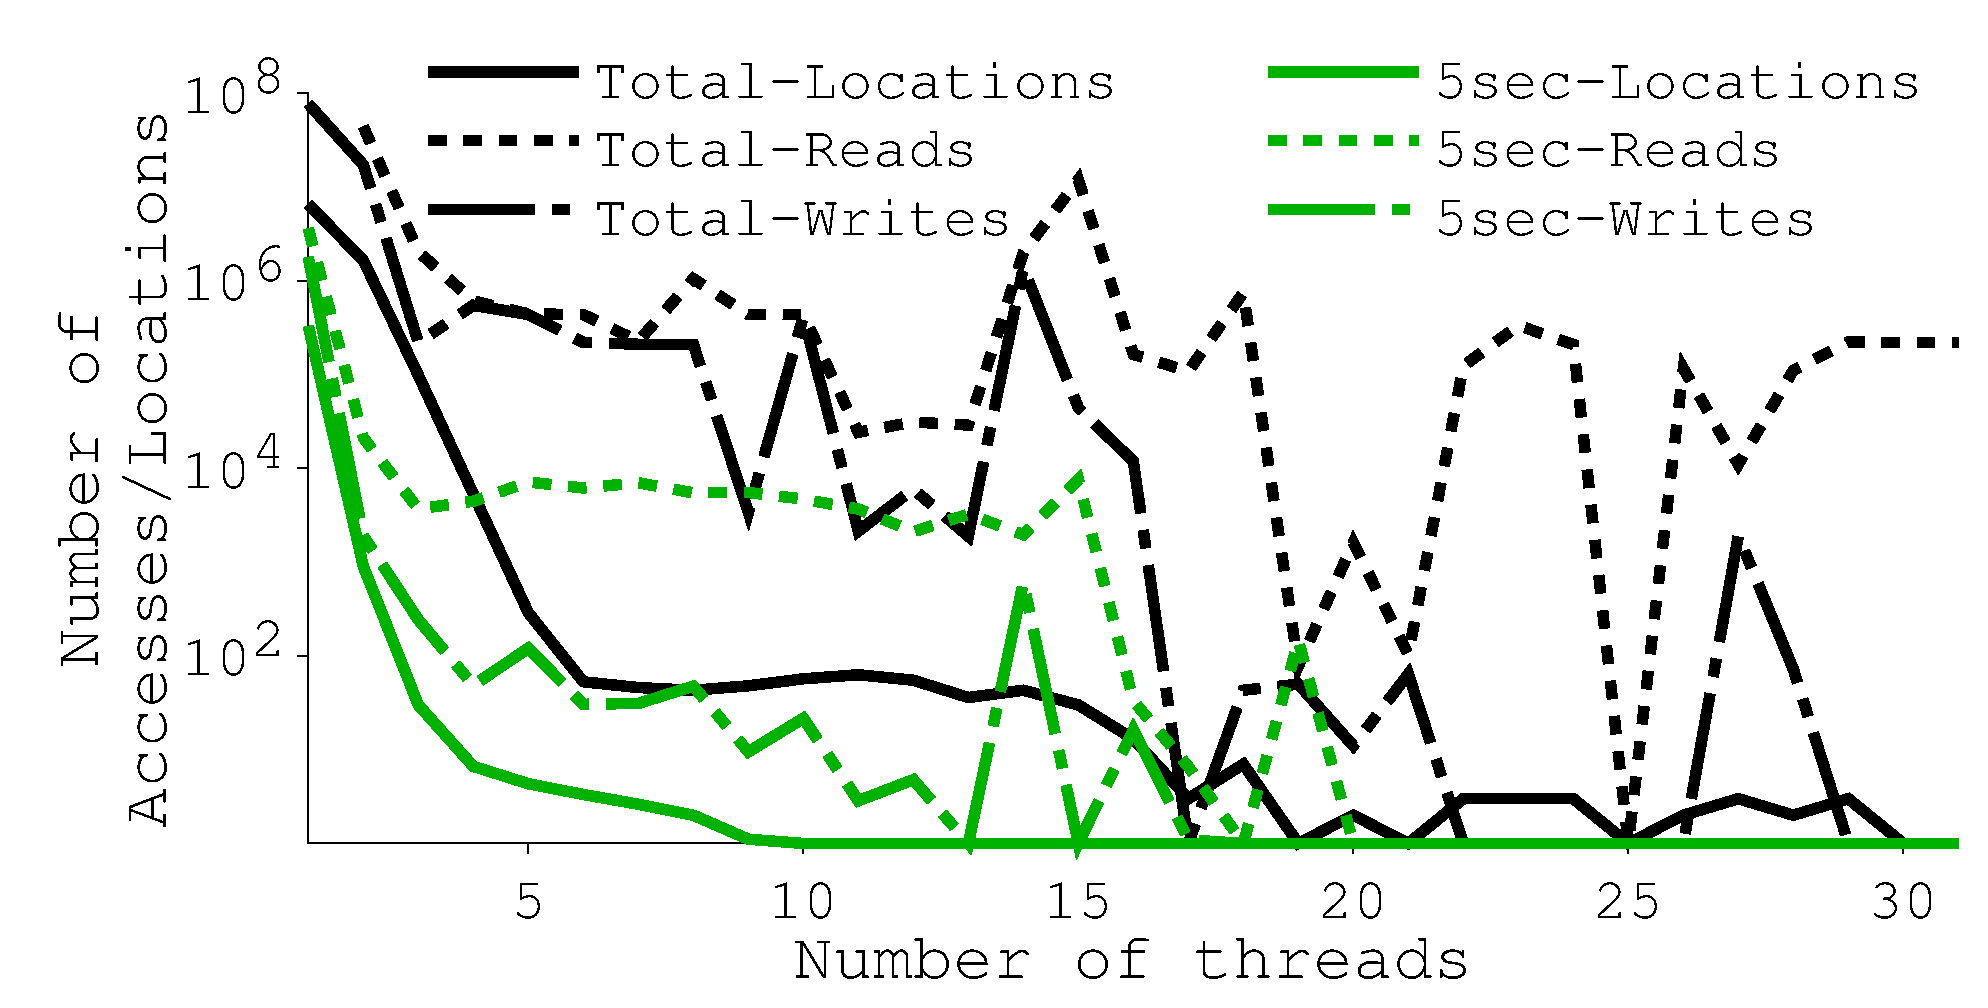
\includegraphics[width=2in]{Figures/g_plot_pagerank_average.pdf}}
%DIFDELCMD < \vspace{-0.1in}
%DIFDELCMD < \mycaption{fig-pagerank}{PowerGraph Sharing Analysis.}
%DIFDELCMD < {
%DIFDELCMD < %%%
\DIFdelFL{Results of running PageRank~\mbox{%DIFAUXCMD
\cite{PageRank} }%DIFAUXCMD
on a Twitter graph~\mbox{%DIFAUXCMD
\cite{Kwak10-WWW}}%DIFAUXCMD
.
%DIF < Number of PowerGraph Pagerank memory reads and writes that are performed by $N$ threads to a shared location,
%DIF < and the number of such shared locations.
Black lines represent total amount of sharing.
Green lines represent sharing within five seconds.
}%DIFDELCMD < }
%DIFDELCMD < \end{center}
%DIFDELCMD < \end{minipage}
%DIFDELCMD < \begin{minipage}{0.01in}
%DIFDELCMD < %%%
\DIFdelFL{\hspace{0.01in}
}%DIFDELCMD < \end{minipage}
%DIFDELCMD < \begin{minipage}{2in}
%DIFDELCMD < \begin{center}
%DIFDELCMD < \centerline{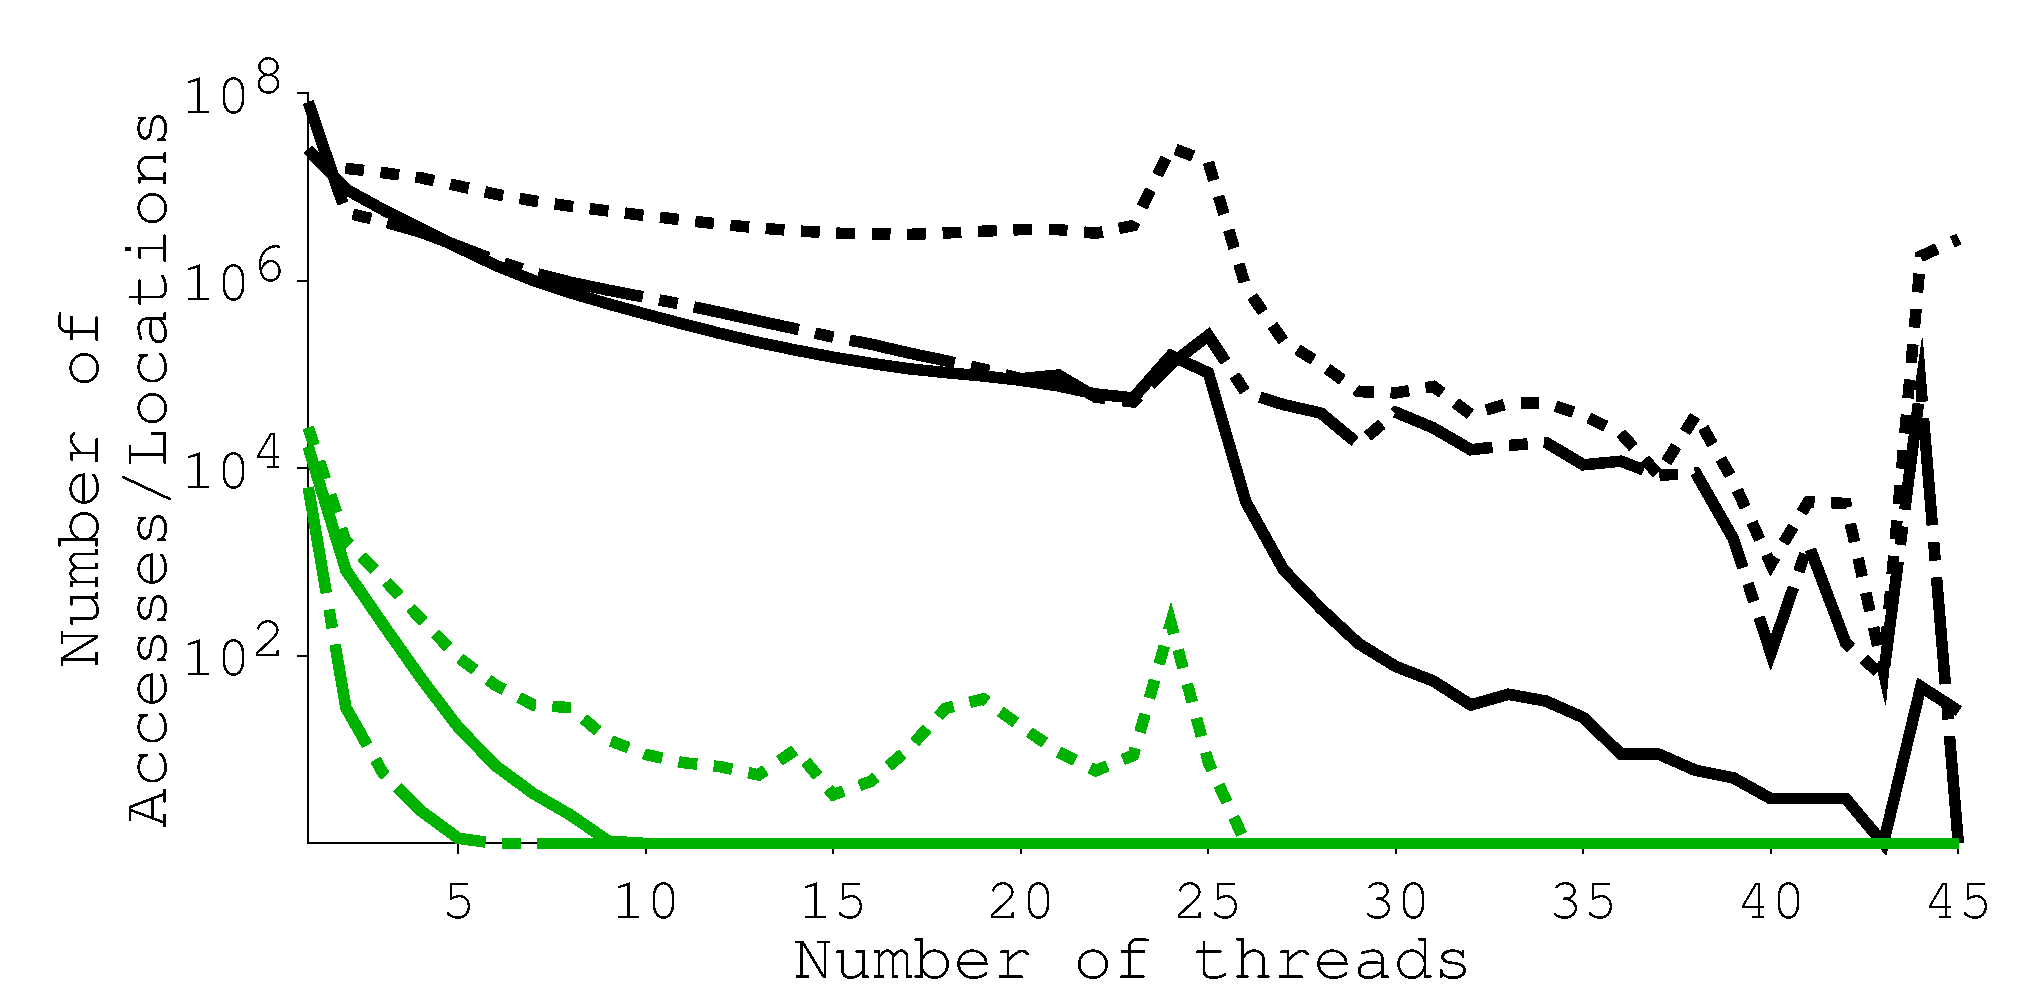
\includegraphics[width=2in]{Figures/g_plot_tensorflow_average.pdf}}
%DIFDELCMD < \vspace{-0.1in}
%DIFDELCMD < \mycaption{fig-tensorflow}{Tensorflow Sharing Analysis.}
%DIFDELCMD < {
%DIFDELCMD < %%%
\DIFdelFL{Results of running a hand-writing recognition workloads provided by TensorFlow.
%DIF < Number of Tensorflow memory reads and writes that are performed by $N$ threads to a shared location,
%DIF < and the number of such shared locations.
Black lines represent total amount of sharing.
Green lines represent sharing within five seconds.
}%DIFDELCMD < }
%DIFDELCMD < \end{center}
%DIFDELCMD < \end{minipage}
%DIFDELCMD < \begin{minipage}{0.01in}
%DIFDELCMD < %%%
\DIFdelFL{\hspace{0.01in}
}%DIFDELCMD < \end{minipage}
%DIFDELCMD < \begin{minipage}{2.3in}
%DIFDELCMD < \begin{center}
%DIFDELCMD < \centerline{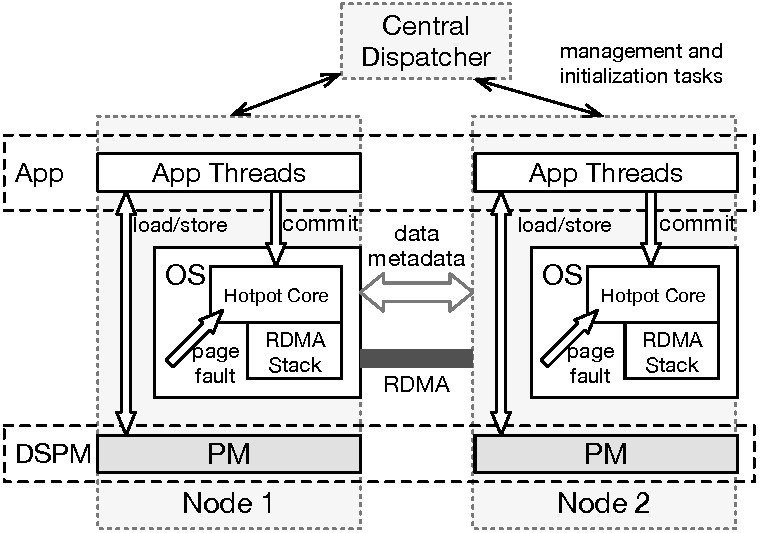
\includegraphics[width=2.3in]{Figures/architecture.pdf}}
%DIFDELCMD < \vspace{-0.1in}
%DIFDELCMD < \mycaption{fig-architecture}{\hotpot\ Architecture.}
%DIFDELCMD < {
%DIFDELCMD < %%%
%DIF < Illustration of \hotpot\ architecture. 
%DIF < \nvm{}s on the two \hotpot\ nodes form a global \dsnvm\ space.
%DIF < An application can run several application threads on each node.
%DIFDELCMD < }
%DIFDELCMD < \end{center}
%DIFDELCMD < \end{minipage}
%DIFDELCMD < \vspace{-0.2in}
%DIFDELCMD < \end{figure*}
%DIFDELCMD < }
%DIFDELCMD < 

%DIFDELCMD < %%%
\DIFdelend Our second idea is to exploit application behaviors and intentions in the \dsnvm\ setting. 
Unlike traditional memory-based applications, persistent-data-based applications,
\dsnvm's targeted type of application, have well-defined data {\em commit points}
where they specify what data they want to make persistent.
When a process in such an application makes data persistent,
it usually implies that the data can be {\em visible} outside the process (\eg, to other processes or other nodes). 
\hotpot\ utilizes these data commit points to also push updates to cached copies on distributed nodes
to avoid maintaining coherence on every \nvm\ write. %~\cite{XXX},
%it is not necessary to maintain memory coherence for each memory access;
%\hotpot\ treats these coherence copies as persistent data replicas
%and makes extra redundant copies to meet the degree of replication specified by users.
%Conducting memory coherence events only at data commit points 
Doing so greatly improves the performance of \hotpot, 
while still ensuring correct memory sharing and data reliability.
%delivering the sharing, reliability, and availability required by \hotpot\ applications. 

%As another example, we employ a replica placement and load balancing technique that relies heavily on application behavior.  


\if 0
\hotpot\ transparently supports memory load and store accesses to both local and remote \nvm\ 
by intercepting the OS page fault handler.
\hotpot\ also supports pointers in \nvm\ and allows applications to use these pointers directly on any \hotpot\ nodes
without any pointer marshaling and unmarshaling.
To let applications name their persistent datasets, \hotpot\ uses a flat namespace with much smaller 
metadata overhead than traditional file system namespaces.

There are no fixed locations for data
eviction: let application access determine
for cold data, goal is to minimize thrashing and minimize impact on hot data, foreground perf
\fi

To demonstrate the benefits of \hotpot, we ported a \DIFdelbegin \DIFdel{NoSql }\DIFdelend \DIFaddbegin \DIFadd{NoSQL }\DIFaddend database, MongoDB~\cite{MongoDB}, to \hotpot\
and built a distributed graph engine similar to PowerGraph~\cite{Gonzalez12-OSDI} on \hotpot\DIFdelbegin \DIFdel{\ (\S\ref{sec:app})}\DIFdelend . 
%We evaluated \hotpot\ with micro-benchmarks, macro-benchmarks, and a real-world large-scale graph.
Our \DIFaddbegin \DIFadd{MongoDB }\DIFaddend evaluation results show that \hotpot\ outperforms \DIFdelbegin \DIFdel{the default MongoDB on }\DIFdelend a \nvm-based system~\cite{Zhang15-Mojim} \DIFdelbegin \DIFdel{, 
an }\DIFdelend \DIFaddbegin \DIFadd{by up to 3.1\x{}, 
two }\DIFaddend NVM-based file \DIFdelbegin \DIFdel{system~\mbox{%DIFAUXCMD
\cite{Dulloor14-EuroSys}}%DIFAUXCMD
}\DIFdelend \DIFaddbegin \DIFadd{systems~\mbox{%DIFAUXCMD
\cite{Dulloor14-EuroSys,Octopus} }%DIFAUXCMD
by up to 787\x{}}\DIFaddend , and a DRAM-based file system \DIFdelbegin \DIFdel{. %DIF <  by up to 787\x{}. 
It }\DIFdelend \DIFaddbegin \DIFadd{by up to 53\x{}. 
\hotpot\ }\DIFaddend outperforms PowerGraph by 2.3\x{} to 5\x{}\DIFdelbegin \DIFdel{and a }\DIFdelend \DIFaddbegin \DIFadd{, a recent }\DIFaddend DSM system~\cite{Nelson15-ATC} by 1.3\x{} to 3.2\x{}\DIFaddbegin \DIFadd{,
and two DSM systems that we built by TODO}\DIFaddend .
%even though PowerGraph adopts sophisticated graph partition techniques 
%and uses two dedicated threads per machine for communication. 
%52\% and 66\% on two real-world graph datasets.
Moreover, \hotpot\ delivers stronger data reliability and availability guarantees than these alternative systems.

\DIFaddbegin \DIFadd{Overall, this paper makes the following key contributions:
}

 \begin{itemize} 
\item \DIFadd{We are the first to introduce the Distributed Shared Persistent Memory (DSPM) model
and among the first to build distributed persistent memory systems.
The DSPM model provides direct and shared memory accesses to a distributed set of \nvm{}s 
and is an easy and viable way for datacenter applications to use \nvm.
}

\item \DIFadd{We propose a one-layer approach to build \dsnvm\ by 
integrating memory coherence and data replication.
The one-layer approach avoids the performance cost of two or more indirection layers.
}

\item \DIFadd{We designed two distributed data commit protocols with different consistency levels 
and corresponding recovery protocols to 
ensure data durability, reliability, and availability.
}

\item \DIFadd{We built the first \dsnvm\ system, \hotpot, in the Linux kernel, 
and two traditional kernel-level DSM systems (as comparison to \hotpot). 
Both \hotpot\ and the two DSM systems are open source.
}

\item \DIFadd{We demonstrated \hotpot's performance benefits and ease of use with two real datacenter applications
and extensive microbenchmark evaluation. 
We compared \hotpot\ with five existing file systems and distributed memory systems, 
and two in-house DSM systems.
}

 \end{itemize} 

\DIFadd{The rest of the paper is organized as follows.
Section 2 presents and analyzes several recent datacenter trends that motivated our design of DSPM.
We discuss the benefits and challenges of DSPM in Section 3.
Section 4 presents the architecture and abstraction of Hotpot.
We then discuss Hotpot's data management in Section 5.
We present our protocols and mechanisms to ensure data durability, consistency, reliability, and availability in Section 6.
Section 7 briefly discusses the network layer we built underlying \hotpot,
and Section 8 presents detailed evaluation of Hotpot.
We cover related work in Section 9 and conclude in Section 10.
}







\DIFaddend \if 0
In summary, we make the following contributions:
 \begin{itemize} [noitemsep]
\item We introduce the DSPM model, which provides direct and shared memory access to a distributed set of PMs.
\item We integrate memory coherence and data replication in one layer.
\item We build the first DSPM system, \hotpot, and demonstrated its benefits with modern data-intensive applications.
 \end{itemize} 


The rest of the paper is organized as follows. Section 2 discusses the background and recent trends toward DSPM.
Section 3 presents the architecture and detailed design of Hotpot. Section 4 presents the ported applications and
evaluation of Hotpot. Section 5 discusses related work. And section 6 concludes.

\dsnvm{}s require both memory coherence {\em and} data replication.
Because applications can access and share \nvm\ like memory, 
\dsnvm{}s need to provide the coherence across multiple copies of data at different nodes' \nvm{}s.
At the same time, applications can also treat these data in \nvm{}s as persistent data, 
which necessitates data replication to provide reliability and high availability.

We propose to integrate memory coherence and data replication in \dsnvm, 
in order to meet the above requirements and to reduce the performance overhead 
caused by redundant indirection~\cite{Nameless}.
When an application process on a node accesses a remote \nvm\ page,
\dsnvm\ will fetch the memory page to the \nvm\ in the local node. 
This local copy serves two simultaneous purposes.
First, the application process can access it locally without any network delay.
Second, by placing the fetched copy in \nvm, it can be treated as a persistent replica 
of the remote \nvm\ page.
To further reduce performance overhead, we will design a set of new mechanisms
to handle memory coherence and data replication at the same time without
extra indirection.
\fi


\if 0
In summary, we make the following contributions.

%\begin{itemize}
 \begin{itemize} [noitemsep]
\item We are the first to introduce the \dsnvm\ model, which provides direct and shared memory access to a distributed set of \nvm{}s.

\item To the best of our knowledge, we are the first to integrate memory coherence and data replication.

\item We built the first \dsnvm\ system, \hotpot,
and demonstrated its benefits with modern data-intensive applications.

 \end{itemize} 
\fi



















\if 0
A unique challenge among these issues is the problem of memory coherence and data replication. 

Although both memory coherence and data replication involve multiple copies of data
and provide various levels of consistency across those copies,
these two techniques have several fundamental differences.
%including different . 
For example, 
when application processes or threads share data and cache multiple copies of that data, 
memory coherence techniques passively maintain consistency across these copies.
Data replication, on the other hand, proactively makes replicas of data to provide redundancy.
Coherence techniques are designed for volatile data,
and clean cached data can be safely thrown away,
while data replication is designed for persistent data and losing data in storage systems is catastrophic.
\fi


%\hotpot\ the abstraction of 
%Applications running on \dsnvm\ directly access \nvm\ with memory load and store 
%instructions for both local and remote \nvm.
%We give full control of how users want to use PM to applications.
% which provides both the ease and performance of direct 
%memory accesses 
%and the reliability and availability of distributed storage systems.

%how to ensure different versions (replica, coherence) do not affect each other, 
%and can convert from each other
%targeted applications


%Combining coherence and replication is not straightforward and has many challenges
%one challenge we met is
%For example, in traditional data replication, once a data has been replicated, 

%one potential problem with \dsnvm\ is


\if 0
Extending this basic idea, we will build a \dsnvm\ system, \hotpot, 
to provide applications with easy-to-use abstraction, native memory accesses, 
low-latency performance, data reliability, consistency, and availability.
We will implement \hotpot\ in Linux on a real Infiniband-based cluster in the PI's lab
and evaluate it with micro-benchmarks and modern data center applications.

Memory coherence and data replication are two important techniques in memory and storage systems.

Memory coherence (or cache coherence) guarantees the consistency of multiple copies of cached data through concurrent accesses.
%for example, by pushing changes from one copy to other copies of the data.
Over the past few decades, researchers have proposed many coherence 
protocols~\cite{Gharachorloo90-ISCA,Gibbons91-SPAA,Kontothanassis97-ISCA,Katz85-ISCA,Gamsa99-OSDI,Srbljic97-IEEE,Mellor-Crummey91-ACM,Tartalja95-HICSS,Gharachorloo90-ISCA,Keleher92-ISCA,Lenoski90-ISCA,Dubois88-IEEE,Li89-ACM,Tomasevic94-IEEE}
%with different tradeoffs of consistency level, performance, and scalability~\cite{}.
and these have been used extensively in local and distributed shared memory systems.

Data replication adds redundancy to persistent data to provide data reliability and availability
in the event of device or machine failure.
Many different data replication techniques  
%offer different levels of data consistency, availability, and performance
are used in local and distributed storage
systems~\cite{AdyaEtAl-Farsite,calder11-azure,DeCandia+07-Dynamo,Ghemawat03-GoogleFS,Gray96-Danger,HellersteinEtAl94-Coding,KubiEtAl00-Ocean,PattersonEtAl88-RAID,Petersen97-Bayou,Rhea03-Pond,Rowstron01-PAST,vanRenesse04-OSDI,Zhong08-Replication}.
%where we intentionally create multiple copies of the data to provide reliability and availability.

Both memory coherence and data replication involve multiple copies of data
and provide various levels of consistency across those copies.
However, the two techniques have several fundamental differences. 

First, memory coherence and data replication have different rationales and use cases.
When application processes or threads share data and cache multiple copies of that data, 
memory coherence techniques passively maintain consistency across these copies.
Data replication, on the other hand, proactively makes replicas of data to provide redundancy.
Second, coherence techniques are designed for volatile data, 
while data replication is designed for persistent data.
Clean cached data can be safely thrown away, while losing data in storage systems is catastrophic.
Finally, memory coherence and data replication operate at different levels of granularity:  
memory coherence granularity exists at the level of a cache line or a memory page, 
while data replication provides granularity at the level of data blocks.


Because of these differences, memory coherence and data replication have always been viewed as orthogonal techniques,
and design decisions reflect that distinction. 
For example, most memory coherence implementations take place in hardware, because memory coherence events usually happen with every memory access
and thus require very low performance overhead.
%Low-latency memory coherence events are thus critical to application performance, 

On the other hand, data replication usually happens when applications commit a set of data (\eg, with \fsync).
Since storage devices are much slower than memory, considerations such as transactional support and 
fast crash recovery often take priority over low-latency replication performance.
As a result,  data replication is most often implemented in user-level software.

%Thus, data replication needs to maintain a certain degree of redundancy for all the persistent data, 
%while there is no such requirement for memory coherence.
%For example, during cache or memory replacement, we can just through away clean data.
%But if we lose or through away a replica, then the replication degree cannot meet user requirements or sustain enough failure.
%there has always been a clean separation between memory and storage, 
%With the advent of \nvm, we raise the question if we should and how to combine coherence and replication.

Recently, emerging disruptive hardware technologies have challenged this long-standing separation between coherence and replication.
Next-generation fast, byte-addressable, non-volatile memories~\cite{NVMDB}
such as 3DXpoint~\cite{Intel3DXpoint}, phase change memory ({\em PCM}),
spin-transfer torque magnetic memories ({\em STTMs})~\cite{SamsungSTTM}, and the memristor~\cite{HP-TheMachine}
can be attached to the main memory bus to form persistent main memory ({\em \nvm}).
%\nvm{}s are blurring the line between memory and storage.

\nvm{}s require both memory coherence {\em and} data replication.
Because applications can access \nvm\ like memory, \nvm{}s need to provide memory coherence across multiple copies of data.
At the same time, applications can also store persistent data in \nvm, 
which necessitates data replication to provide reliability and high availability.
The need for both memory coherence and data replication is especially 
acute in distributed datacenter environments, where large-scale applications
access and share a vast amount of data that are distributed across nodes.
%These environments raise the need for both memory coherence and data replication.
%and the separation of memory coherence and data replication.
%Applications can access \nvm{}s with memory load and store instructions
%and at the same time use \nvm{}s to store persistent data.
%Such usage scenarios raise the need for both memory coherence and data replication.
%This paper explores the challenges of providing coherence and data replication to \nvm.

We introduce {\em Distributed Shared Persistent Memory (\dsnvm)}, 
a framework that uses a pool of machines with \nvm{}s to form a global, shared, and persistent memory space.
Applications can perform traditional memory load and store instructions to access both local and remote data in this global memory space 
and can at the same time make their data persistent and reliable.
\dsnvm\ provides an easy-to-use model that can potentially meet modern datacenter applications' demand for low-latency, shared memory access, data reliability, and high availability. 
A fundamental challenge of \dsnvm\ is efficiently maintaining memory coherence and
data replication, while providing performance that is close to local \nvm\ in spite of network delay.

We propose to integrate memory coherence and data replication in \dsnvm, 
in order to meet the above requirements.
When an application process on a node accesses a remote \nvm\ page,
\dsnvm\ will fetch the memory page to the \nvm\ in the local node. 
This local copy serves two simultaneous purposes.
First, the application process can access it locally without any network delay.
Second, by placing the fetched copy in \nvm, it can be treated as a persistent replica 
of the remote \nvm\ page.
%The only difference between coherent and redundant copies is that
%coherent copies have been accessed by applications and thus are visible to applications, 
%while redundant copies 
\fi

%The rest of the paper is organized as follows. 
%Section~\ref{}

\DIFdelbegin %DIFDELCMD < \vspace{-0.05in}
%DIFDELCMD < %%%
\DIFdelend \section{Motivation}
\label{sec:motivation}
\DIFdelbegin %DIFDELCMD < \vspace{-0.05in}
%DIFDELCMD < %%%
\DIFdelend 

%DIF < We introduce {\em Distributed Shared Persistent Memory (\dsnvm)},
%DIF < a framework to use \nvm\ in distributed datacenter environments.
\dsnvm\ is motivated by three datacenter trends: 
emerging hardware \nvm\ technologies, 
modern data-intensive applications' data sharing, persistence, and reliability needs, 
and the availability of fast datacenter network.
%DIF < applications' increasing demands for high availability and data reliability.
%DIF < This section presents a case for \dsnvm,
%DIF < and discusses the motivation, opportunities, and challenges of \dsnvm.

\DIFdelbegin %DIFDELCMD < \vspace{-0.05in}
%DIFDELCMD < %%%
\DIFdelend \subsection{Persistent Memory and PM Apps}
\DIFdelbegin %DIFDELCMD < \vspace{-0.05in}
%DIFDELCMD < %%%
%DIF < why we should support load store
\DIFdelend Next-generation non-volatile memories ({\em NVMs}), 
such as 3DXpoint~\cite{Intel3DXpoint}, phase change memory ({\em PCM}),
spin-transfer torque magnetic memories ({\em STTMs}), and the memristor
will provide byte addressability, persistence, and latency that is within 
an order of magnitude of 
DRAM~\DIFdelbegin \DIFdel{\mbox{%DIFAUXCMD
\cite{hosomi2005novel,Lee10-pcmquest,lee2010phase,lee2011fast,pcmdataasheet,qureshi2010morphable,NVMDB,yang2013memristive}}%DIFAUXCMD
}\DIFdelend \DIFaddbegin \DIFadd{\mbox{%DIFAUXCMD
\cite{hosomi2005novel,Lee10-pcmquest,lee2010phase,lee2011fast,pcmdataasheet,qureshi2010morphable,NVMDB,yang2013memristive,Octopus}}%DIFAUXCMD
}\DIFaddend .
These developments are poised to radically alter the landscape of memory and storage technologies.
%DIF < and have already inspired a host of research 
%DIF < projects~\cite{Bailey10-OSImpl,Coburn11-ASPLOS, sosp09:bpfs, Dulloor14-EuroSys, hotos09:mogul, MemoryPersistency,Volos11-ASPLOS, Xiaojian11-SC}.

NVMs can attach directly to the main memory bus to form Persistent Memory. 
If applications want to exploit all the low latency and byte-addressability benefits of \nvm,
they should directly access it via memory load and store instructions without any software 
overheads~\cite{Coburn11-ASPLOS,Volos11-ASPLOS,Zhang15-Mojim,Memory-Persistency,Kamino-EuroSys17,pmxact-asplos16} 
(we call this model {\em durable in-memory computation}),
%DIF < without operating system overheads for most accesses
rather than accessing it via a file system~\cite{sosp09:bpfs,Dragojevic14-NSDI,Dulloor14-EuroSys,Xiaojian11-SC,HiNFS-Eurosys16}.

\DIFdelbegin \DIFdel{Unfortunately, }\DIFdelend \DIFaddbegin {
\begin{figure}[th]
\begin{center}
\centerline{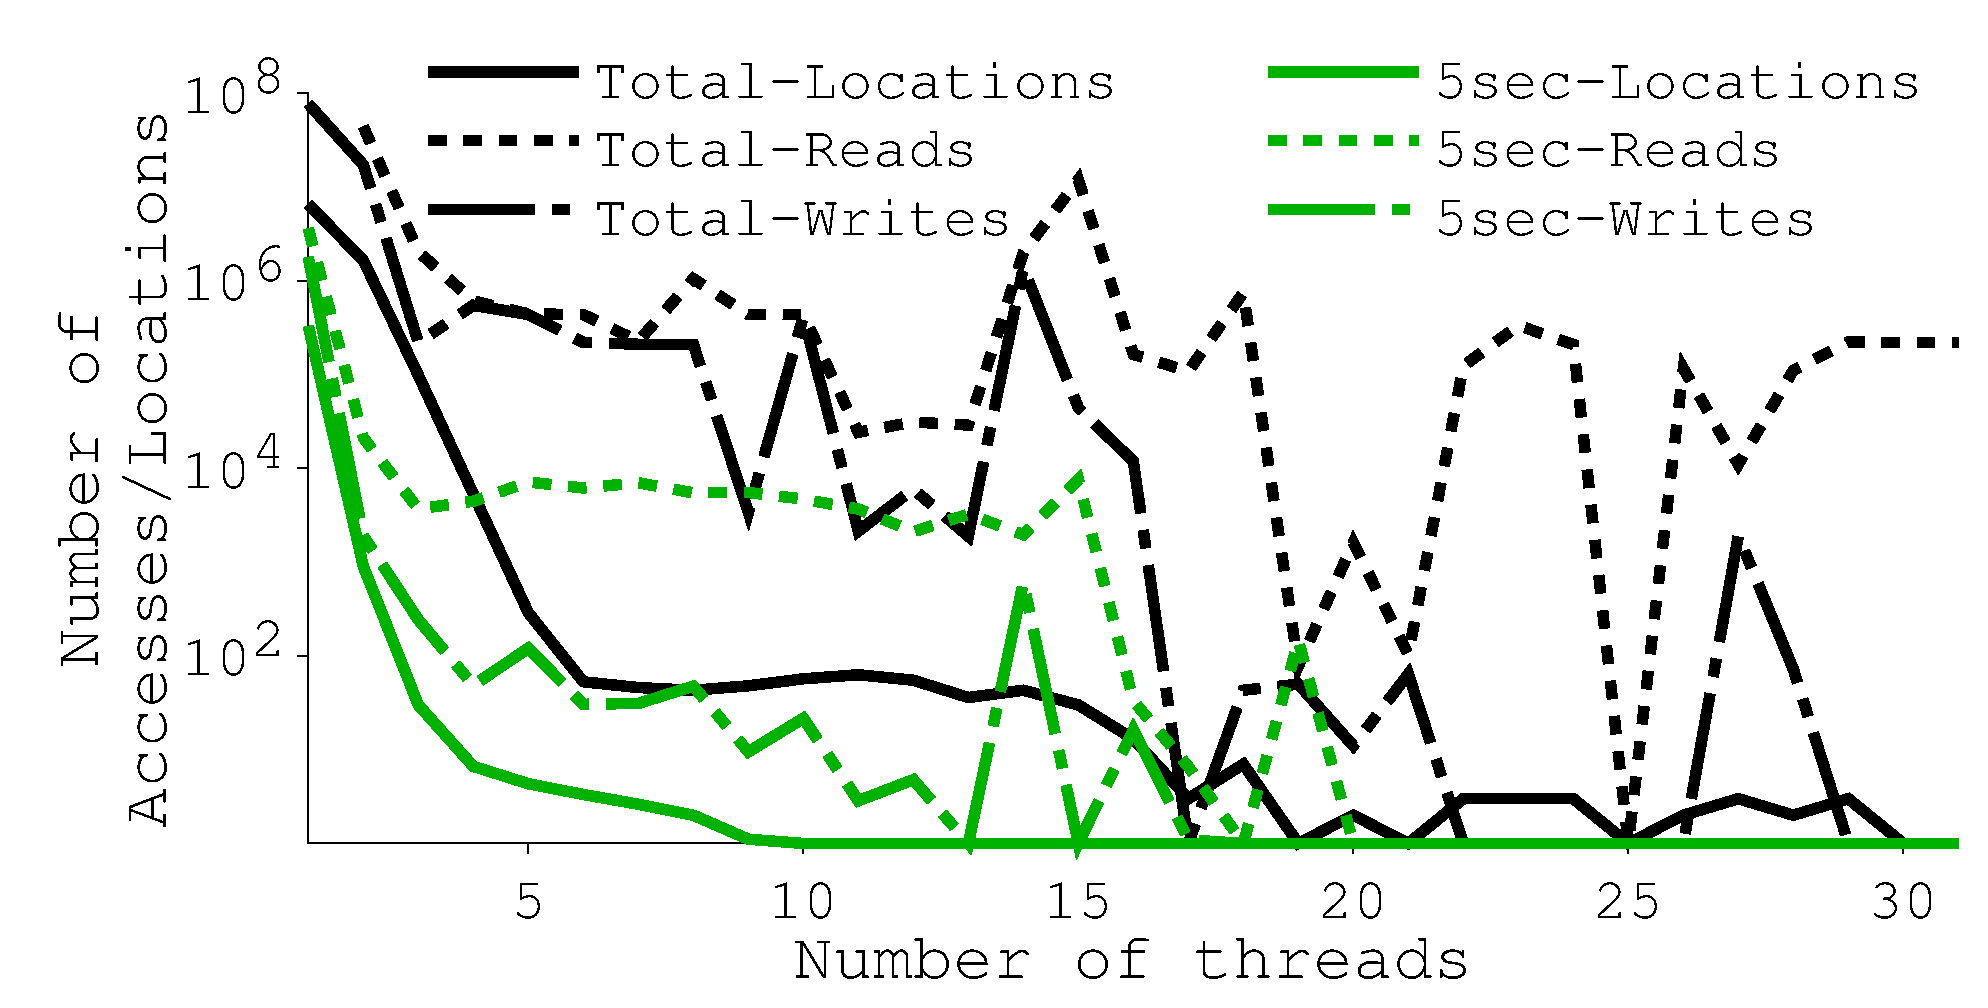
\includegraphics[width=0.5\textwidth]{Figures/g_plot_pagerank_average.pdf}}
\mycaption{fig-pagerank}{PowerGraph Sharing Analysis.}
{
\DIFaddFL{Results of running PageRank~\mbox{%DIFAUXCMD
\cite{PageRank} }%DIFAUXCMD
on a Twitter graph~\mbox{%DIFAUXCMD
\cite{Kwak10-WWW}}%DIFAUXCMD
.
%DIF > Number of PowerGraph Pagerank memory reads and writes that are performed by $N$ threads to a shared location,
%DIF > and the number of such shared locations.
Black lines represent total amount of sharing.
Green lines represent sharing within five seconds.
}}
\end{center}
\end{figure}
}

\DIFadd{Unfortunately, most }\DIFaddend previous durable in-memory systems were \DIFdelbegin \DIFdel{all }\DIFdelend designed for the single-node environment\DIFdelbegin \DIFdel{and there is no distributed support for them.
%DIF <  (other than our own previous work which provides efficient \nvm\ replication~\cite{Zhang15-Mojim}).
}\DIFdelend \DIFaddbegin \DIFadd{.
%DIF > and there is no distributed support for them.
}\DIFaddend With modern datacenter applications' computation scale, 
we have to be able to scale out these \DIFdelbegin \DIFdel{applications.
%DIF < To scale out these applications, we need a 
}\DIFdelend \DIFaddbegin \DIFadd{single-node \nvm\ systems.
}\DIFaddend 

\DIFdelbegin %DIFDELCMD < \vspace{-0.05in}
%DIFDELCMD < %%%
\DIFdelend \subsection{Shared Memory Applications}
\DIFdelbegin %DIFDELCMD < \vspace{-0.05in}
%DIFDELCMD < %%%
\DIFdelend Modern data-intensive applications increasingly need
to access and share vast amounts of data fast. 
%DIF < XXX memory-based
%DIF < Most of these data-intensive applications rely heavily on parallelism to achieve high throughput
%DIF < when accessing and processing data.
We use PIN~\cite{Luk05-PLDI} to collect memory access traces of two popular data-intensive applications, 
TensorFlow~\cite{TensorFlow} and PowerGraph~\cite{Gonzalez12-OSDI}.
%DIF < running a hand-writing recognition workloads provided by TensorFlow
%DIF < and PageRank~\cite{PageRank} on a Twitter graph~\cite{Kwak10-WWW} respectively. 
%DIF < We analyzed various memory-sharing properties of these memory traces.
Figures~\ref{fig-pagerank} and \ref{fig-tensorflow} show the total number of reads and writes performed to the same memory location 
by $N$ threads and the amount of these shared locations.
There are a significant amount of shared read accesses in these applications,
especially across a small set of threads.
%DIF < For both TensorFlow and PowerGraph, a large number of threads have many shared reads to a few locations.
We further divided the memory traces into smaller time windows 
and found that there is still a significant amount of sharing, 
indicating that many shared accesses occur at similar times. 

Distributed Shared Memory ({\em \dsm}) takes the shared memory concept a step further 
by organizing a pool of machines into a globally shared memory space.
%DIF < \subsection{Distributed Shared Memory}
Researchers and system builders have developed a host of software and hardware \dsm\ systems in the past few 
decades~\cite{Bennett90-PPOPP,Bisiani90-ISCA,Black89-COMPCON,Delp:1988:AIM:59505,Fleisch89-SOSP,Gibbons91-SPAA,Kontothanassis97-ISCA,Lo94-AC,Kessler89-ACM,Stumm90-IEEE,Keleher92-ISCA,Ramachandran91-Wiley,Zhou92-IEEE,Zhou92-IEEE,Stumm90-IEEE,Stumm90-IPDPS,HLRC,Shasta}.
%DIF < However, usage of these \dsm\ systems has been limited, 
%DIF < mainly because their high network and software overheads are not acceptable for most memory-based applications.
\DIFdelbegin \DIFdel{Recently, %DIF < with the increasing popularity of low-latency RDMA networks in data centers~\cite{Dragojevic14-NSDI,Kalia14-SIGCOMM,Wei15-SOSP}, 
}\DIFdelend \DIFaddbegin \DIFadd{Recently, }\DIFaddend there is a new interest in \dsm~\cite{Nelson15-ATC} to support modern data-intensive applications.

However, although DSM scales out shared-memory applications, 
there has been no persistent-memory support for DSM.
DSM systems all had to checkpoint to disks~\cite{Stumm90,Richard93,Neves94}.
Memory persistence
%DIF < offers at least two benefits to existing in-memory applications.
can allow these applications to checkpoint fast and recover fast~\cite{Narayanan12-ASPLOS}.
%DIF < In addition, deploying applications on \nvm\ can allow them to access more in-memory data,
%DIF < since \nvm\ offers higher capacity than DRAM.

\DIFdelbegin %DIFDELCMD < \vspace{-0.05in}
%DIFDELCMD < %%%
\DIFdelend \subsection{Fast Network and RDMA}
\DIFdelbegin %DIFDELCMD < \vspace{-0.05in}
%DIFDELCMD < %%%
\DIFdelend Datacenter network performance has improved significantly over the past decades.
%DIF < seen significant advances in both performance and functionality in the past decade.
InfiniBand ({\em \ib}) NICs and switches support high bandwidth ranging from 40 to 100\gbps.
%DIF < There is also a great interest to push towards high bandwidth Ethernet~\cite{MellanoxETH}.
Remote Direct Memory Access ({\em RDMA}) technologies that provide low-latency remote memory accesses
have become more mature for datacenter uses in recent years~\cite{FaSST,Dragojevic14-NSDI,Kalia14-SIGCOMM,Guo16-SIGCOMM}.
%DIF < They enable fast remote memory accesses and have already inspired several distributed 
%DIF < memory and storage systems
%DIF < Moreover, \ib\ supports lossless and ordered communication and can potentially 
%DIF < simplify many distributed systems protocols~\cite{ApproxSynchrony}.
These network technology advances
%DIF < enable faster distributed storage systems
make remote-memory-based systems~\cite{Nelson15-ATC,GU17-NSDI,OSDI-Disaggregate,Chen16-EUROSYS,Binnig16-VLDB,Zamanian17-VLDB} more attractive than decades ago.
%DIF < it will be both more efficient and easier to build 
%DIF < distributed memory and distributed storage systems.

\DIFdelbegin %DIFDELCMD < \vspace{-0.05in}
%DIFDELCMD < %%%
\DIFdelend \DIFaddbegin {
\begin{figure}[th]
\begin{center}
\centerline{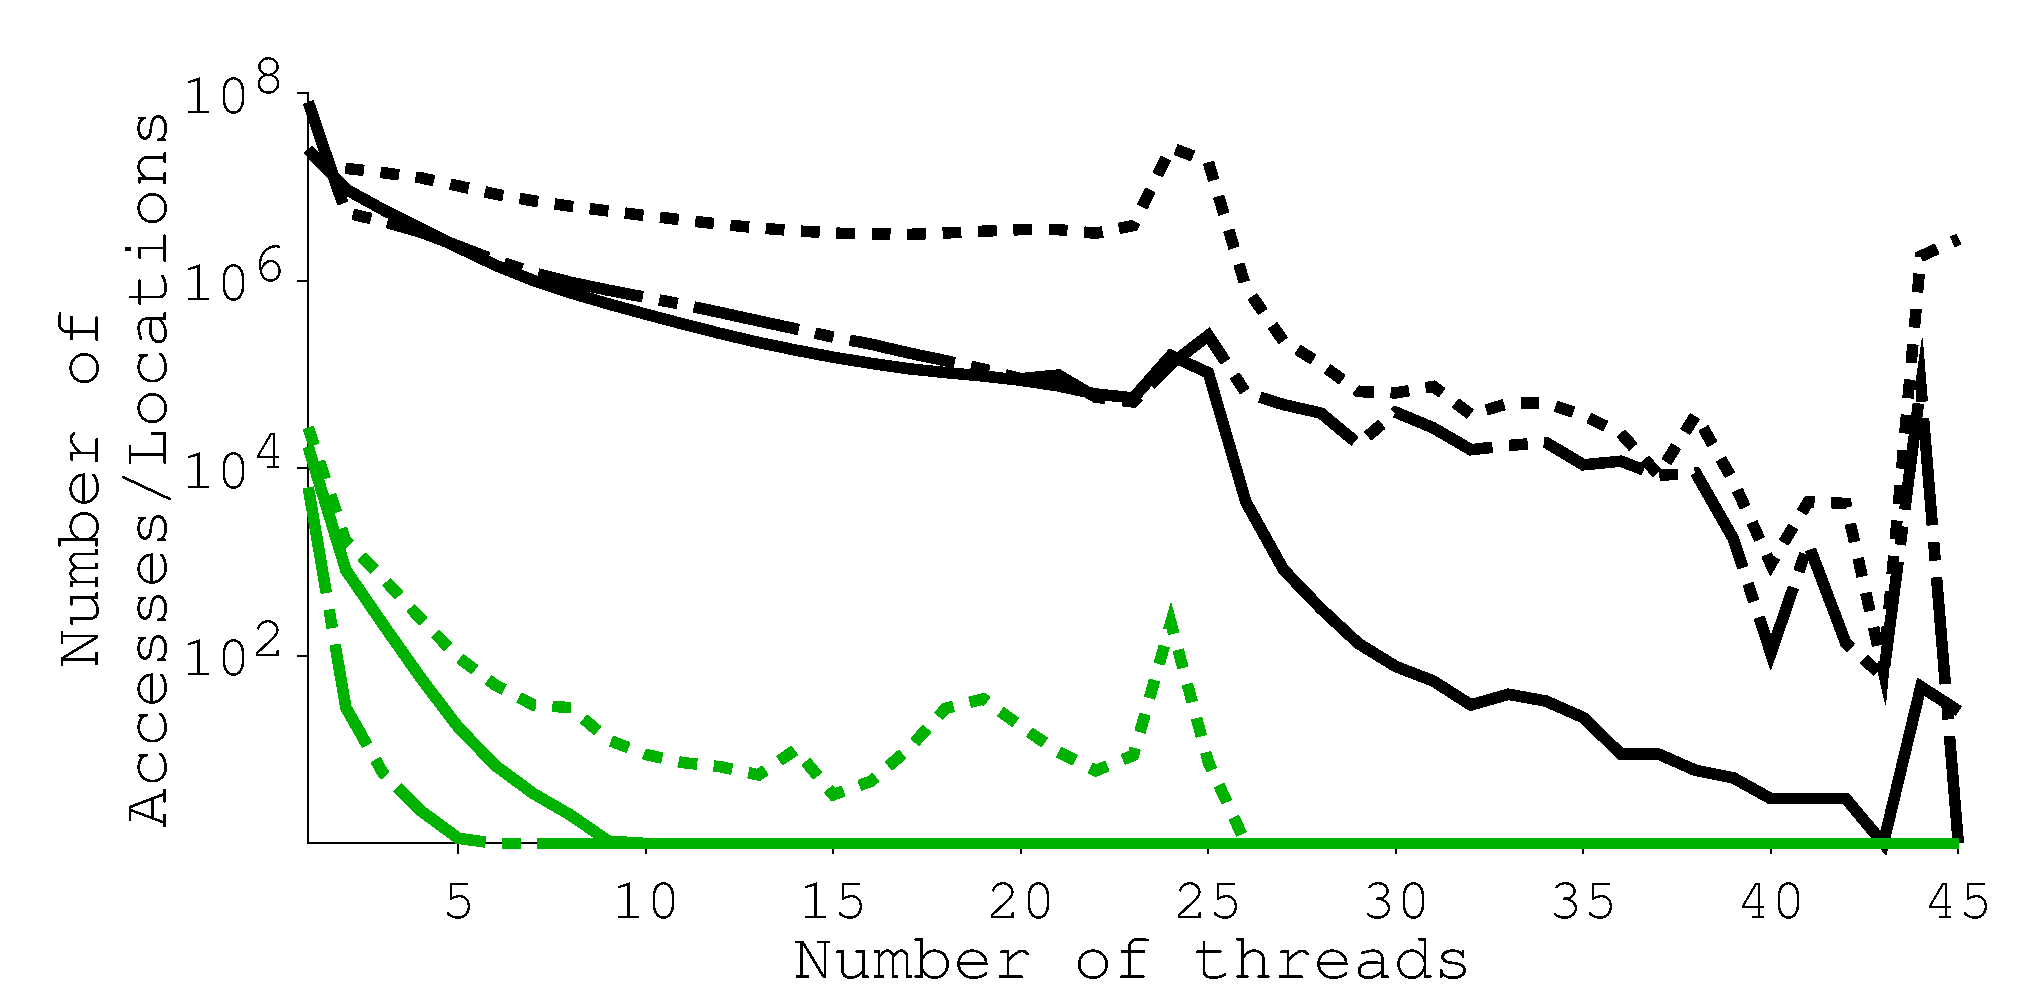
\includegraphics[width=0.5\textwidth]{Figures/g_plot_tensorflow_average.pdf}}
\mycaption{fig-tensorflow}{Tensorflow Sharing Analysis.}
{
\DIFaddFL{Results of running a hand-writing recognition workloads provided by TensorFlow.
%DIF > Number of Tensorflow memory reads and writes that are performed by $N$ threads to a shared location,
%DIF > and the number of such shared locations.
Black lines represent total amount of sharing.
Green lines represent sharing within five seconds.
}}
\end{center}
\end{figure}
}

\DIFaddend \subsection{Lack of Distributed PM Support}
\DIFdelbegin %DIFDELCMD < \vspace{-0.05in}
%DIFDELCMD < %%%
\DIFdelend \if 0
Almost all datacenters use distributed data storage systems to store persistent data~\cite{AdyaEtAl-Farsite,calder11-azure,DeCandia+07-Dynamo,Ghemawat03-GoogleFS,KubiEtAl00-Ocean,Petersen97-Bayou}.
In these datacenter environments, software, hardware, and networking errors 
are common~\cite{ford2010availability,nath06-subtleties}. 
To ensure that applications do not lose their data and can always access them even when these errors happen, 
distributed storage systems 
add data redundancy or replication. 
A host of distributed data storage systems  
offer different levels of data consistency, availability, 
and performance~\cite{AdyaEtAl-Farsite,calder11-azure,DeCandia+07-Dynamo,Ghemawat03-GoogleFS,KubiEtAl00-Ocean,Petersen97-Bayou}.
\fi
\DIFaddbegin 

\DIFaddend Many large-scale datacenter applications require fast access to vast amounts of persistent data
and could benefit from \nvm's performance, durability, and capacity benefits.
For \nvm{}s to be successful in datacenter environments, they have to support these applications.
%DIF < are especially apparent in datacenter environments,
However, neither traditional distributed storage systems or DSM systems are designed for \nvm.
Traditional distributed storage systems~\cite{AdyaEtAl-Farsite,calder11-azure,DeCandia+07-Dynamo,Ghemawat03-GoogleFS,KubiEtAl00-Ocean,Petersen97-Bayou}
target slower, block-based storage devices.
Using them on \nvm{}s will result in excessive software and network overheads that outstrip \nvm's low latency performance~\cite{Zhang15-Mojim}.
DSM systems were designed for fast, byte-addressable memory, but lack the support for data durability and reliability.
%DIF < There are a host of distributed data storage systems that support different consistency, reliability, availability, and performance 
%DIF < requirements for persistent data applications~\cite{AdyaEtAl-Farsite,calder11-azure,DeCandia+07-Dynamo,Ghemawat03-GoogleFS,KubiEtAl00-Ocean,Petersen97-Bayou}.
%DIF < However, these traditional distributed storage systems are designed for slower storage devices.
%DIF < A recent work~\cite{Zhang15-Mojim} proposed an efficient way to replicate \nvm.

\DIFdelbegin %DIFDELCMD < \vspace{-0.05in}
%DIFDELCMD < %%%
\DIFdelend \DIFaddbegin \DIFadd{Octopus~\mbox{%DIFAUXCMD
\cite{Octopus} }%DIFAUXCMD
is a recent RDMA-enabled distributed file system built for PM.
Octopus was developed in parallel with \hotpot\ and has a similar goal as \hotpot: 
to manage and expose distributed PM to datacenter applications. 
However, Octopus uses a file system abstraction and is built in the user level.
These designs add significant performance overhead to native PM accesses (Section~\ref{sec:mongodb}).
Moreover, Octopus does not provide any data reliability or high availability, 
both of which are key requirements in datacenter environments.
%DIF > it scales out from single-node environment to
%DIF > manage a pool of distributed PM, and provides applications with direct access to shared PM
%DIF > through data I/O. However, in Octopus, the special byte-addressable property of PM is not fully exposed to
%DIF > applications.
}

\DIFaddend \section{\dsnvm}
%DIF < Distributed Shared Persistent Memory}
\label{sec:dspm}
\DIFdelbegin %DIFDELCMD < \vspace{-0.05in}
%DIFDELCMD < %%%
\DIFdelend 

The datacenter application and hardware trends described in \S\ref{sec:motivation} 
clearly point to one promising direction of using \nvm\ in datacenter environments --- 
%DIF < From the above analysis, it is clear that 
%DIF < Modern datacenter applications need to store, access, and share 
%DIF < more data than is feasible with a single machine.
%DIF < To meet these application needs, we propose using 
as distributed, shared, persistent memory (\dsnvm).
A \dsnvm\ system manages a distributed set of \nvm{}-equipped machines  
and provides the abstraction of a global virtual address space and a data persistence interface to applications.
%DIF < lets applications have native memory load/store access in a global virtual address space
%DIF < and be able to make their data persistent and reliable.

\DIFdelbegin %DIFDELCMD < \vspace{-0.05in}
%DIFDELCMD < %%%
\DIFdelend \subsection{\dsnvm\ Benefits and Usage Scenarios}
\DIFdelbegin %DIFDELCMD < \vspace{-0.05in}
%DIFDELCMD < %%%
\DIFdelend \dsnvm\ offers low-latency, shared access to vast amount of durable data in distributed \nvm,
and the reliability and high availability of these data.
Application developers can build in-memory data structures with the global virtual address space 
and decide how to name their data and when to make data persistent.

Applications that fit \dsnvm\ well have two fundamental properties:
accessing data with memory instructions and making data durable explicitly.
We call the time when an application makes its data persistent a {\em commit point}.
There are several types of datacenter applications that meet the above two descriptions and can benefit from running on \dsnvm.

\DIFaddbegin {
\begin{table}[th]\small
\begin{center}
\begin{center}
\begin{tabular}{ p{0.5in} | p{1.5in} | p{0.6in} }
\small \DIFaddFL{API }& \small \DIFaddFL{Explanation }& \small \DIFaddFL{Backward }\\
\hline
\hline
\DIFaddFL{\open\ (\close) }& \DIFaddFL{open or create (close) a \dsnvm\ dataset }& \DIFaddFL{same as current }\\
\hline
\DIFaddFL{\mmap\ (\unmap) }& \DIFaddFL{map (unmap) a \dsnvm\ region in a dataset to application address space }& \DIFaddFL{same as current }\\
%DIF > \close\ & close a \dsnvm\ dataset & same as file \close\ \\
\hline
\DIFaddFL{\commit\  }& \DIFaddFL{commit a set of data and make $N$ persistent replicas }& \DIFaddFL{similar to msync }\\
\hline
\DIFaddFL{\acquire\  }& \DIFaddFL{acquire single writer permission }& \\
%DIF > \fetch\ & fetch a set of committed data & \\
\hline
%DIF > \commit\ & atomically commit dirty data and make $N$ persistent replicas & same as current \\
%DIF > \hline
\DIFaddFL{\barrier\ }& \DIFaddFL{helper function to synchronzation threads on different nodes }& \DIFaddFL{similar to pthread barrier }\\
\end{tabular}
\end{center}
\mycaption{tbl-apis}{\hotpot\ APIs.}
{
%DIF > APIs \hotpot\ provides to applications, their meaning, and backward compatibility to traditional system calls.
\DIFaddFL{Apart from these APIs, \hotpot\ also supports direct memory loads and stores.
}}
\end{center}
\end{table}

{
\begin{figure}[th]
\begin{center}
\centerline{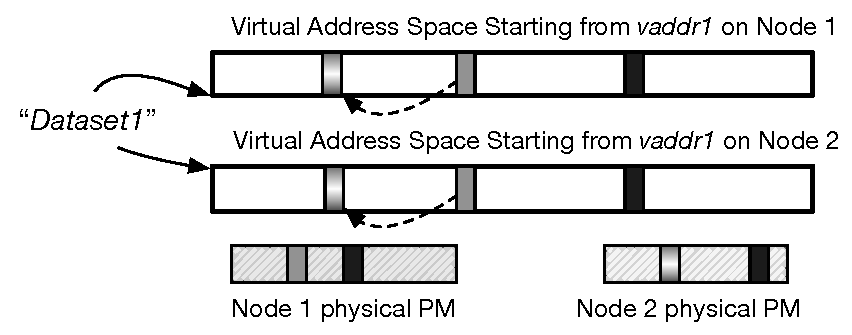
\includegraphics[width=0.5\textwidth]{Figures/addressing.pdf}}
\mycaption{fig-addressing}{\hotpot\ Addressing.}
{
\DIFaddFL{\hotpot\ maps ``}{\em \DIFaddFL{Dataset1}}\DIFaddFL{'' to Node 1 and Node 2's virtual address space using the 
same base virtual addresses. The physical address mapping on each node is different.
The grey blocks in the middle are pointers that point to the blocks on the left. 
}}
\end{center}
\end{figure}
}


\DIFaddend First, applications that are built for single-node \nvm\
can be easily ported to \dsnvm\ and scale out to distributed environments.
%DIF < , since \dsnvm\ will hide all the network communication or distributed states from them.
These applications store persistent data as in-memory data structures 
and already express their commit points explicitly.
%DIF <  (via the set of \nvm\ persistent instructions).
Similarly, storage applications that use memory-mapped \DIFdelbegin \DIFdel{I/Os }\DIFdelend \DIFaddbegin \DIFadd{files }\DIFaddend also fit \dsnvm\ well,
%DIF < ~\cite{MongoDB,XXX} also fit \dsnvm\ well,
since they operate on in-memory data and explicitly make them persistent at well-defined commit points (\ie, \msync).
Finally, \dsnvm\ fits shared-memory or DSM-based applications that desire to incorporate durability.
These applications do not yet have durable data commit points,
but we expect developers to specify when and what they want make durable.

\DIFdelbegin %DIFDELCMD < \vspace{-0.05in}
%DIFDELCMD < %%%
\DIFdelend \subsection{\dsnvm\ Challenges}
\label{sec:challenges}
\DIFdelbegin %DIFDELCMD < \vspace{-0.05in}
%DIFDELCMD < %%%
\DIFdelend Building a \dsnvm\ system presents several new challenges.
%DIF < }most of which result from the need 

First, {\em what type of abstraction should \dsnvm\ offer to support both direct memory accesses and data persistence (\S\ref{sec:abstraction})}?
To perform native memory accesses, application processes should use virtual memory addresses. 
But virtual memory addresses are not a good way to {\em name} persistent data.
\dsnvm\ needs a naming mechanism that applications can easily use to retrieve their in-memory data after reboot or crashes (\S\ref{sec:naming}).
Allowing direct memory accesses to \dsnvm\ also brings another new problem:
pointers need to be both persistent in \nvm\ and consistent across machines (\S\ref{sec:addressing}).

\DIFaddbegin {
\begin{figure}[th]
\begin{center}
\centerline{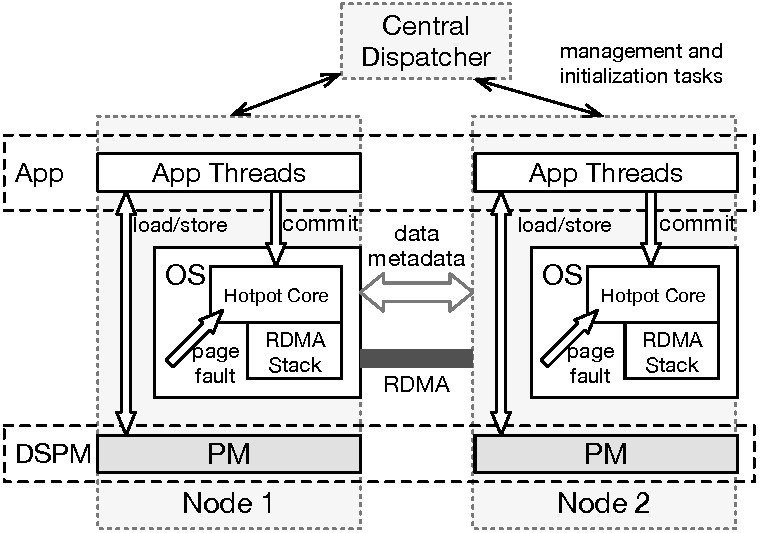
\includegraphics[width=0.5\textwidth]{Figures/architecture.pdf}}
\mycaption{fig-architecture}{\hotpot\ Architecture.}
{
%DIF > Illustration of \hotpot\ architecture. 
%DIF > \nvm{}s on the two \hotpot\ nodes form a global \dsnvm\ space.
%DIF > An application can run several application threads on each node.
}
\end{center}
\end{figure}
}


\DIFaddend Second, {\em how to efficiently organize data in \dsnvm\ to deliver good application performance (\S\ref{sec:data})?}
To make \dsnvm's interface easy to use and transparent, 
\dsnvm\ should manage the physical \nvm\ space for applications and handle \nvm\ allocation.
\dsnvm\ needs a flexible and efficient data management mechanism to deliver good performance to different types of applications.
%DIF < and a balanced, minimal network load.
%DIF < Data and metadata in \dsnvm\ (\S\ref{sec:data})?
%DIF < \dsnvm\ needs to to a large amount of nodes and manage resources and application loads (\S\ref{sec:data})?

Finally, {\em \dsnvm\ needs to ensure both \DIFaddbegin \DIFadd{distributed }\DIFaddend cache coherence and data reliability at the same time} (\S\ref{sec:xact}).
The former requirement ensures the coherence of multiple cached copies \DIFaddbegin \DIFadd{at different machines }\DIFaddend under concurrent accesses and is usually enforced in \DIFdelbegin \DIFdel{the }\DIFdelend \DIFaddbegin \DIFadd{a distributed }\DIFaddend memory layer.
The latter provides data reliability and availability when errors happen and is implemented in \DIFaddbegin \DIFadd{distributed }\DIFaddend storage systems or \DIFaddbegin \DIFadd{distributed }\DIFaddend databases.
\dsnvm\ needs to incorporate both these two different requirements in one layer in a correct and efficient way.
%DIF < Traditionally, 
%DIF < How to minimize performance overhead and exploit the most from \nvm's low latency performance (\S\ref{sec:resource})?
%DIF > Note that PM is attached to main memory bus directly, hence we assume PM share the same CPU cache coherence mechanism with DRAM.
%DIF > Hotpot focus on cache coherence among different cached copies across nodes.

\DIFdelbegin %DIFDELCMD < \vspace{-0.05in}
%DIFDELCMD < \section{\hotpot\ Design}
%DIFDELCMD < %%%
\DIFdelend \DIFaddbegin \section{\hotpot\ Architecture and Abstraction}
\DIFaddend \label{sec:design}
\DIFdelbegin %DIFDELCMD < \vspace{-0.05in}
%DIFDELCMD < %%%
\DIFdelend \DIFaddbegin \label{sec:abstraction}
\DIFaddend 


We propose {\em \hotpot}, a kernel-level \dsnvm\ system that %manages \dsnvm\ and
%manages distributed shared persistent memory
provides applications with direct memory load/store access \DIFdelbegin \DIFdel{access }\DIFdelend to both local and remote \nvm\
and a mechanism to make in-\nvm\ data durable, consistent, and reliable.
\hotpot\ is easy to use, delivers low-latency performance, 
and provides flexible choices of data consistency, reliability, and availability levels.
\DIFdelbegin %DIFDELCMD < 

%DIFDELCMD < {
%DIFDELCMD < \begin{table}[th]\scriptsize
%DIFDELCMD < \begin{center}
%DIFDELCMD < \begin{center}
%DIFDELCMD < \begin{tabular}{ p{0.5in} | p{1.5in} | p{0.6in} }
%DIFDELCMD < \footnotesize %%%
\DIFdelFL{API }%DIFDELCMD < & \footnotesize %%%
\DIFdelFL{Explanation }%DIFDELCMD < & \footnotesize %%%
\DIFdelFL{Backward }%DIFDELCMD < \\
%DIFDELCMD < \hline
%DIFDELCMD < \hline
%DIFDELCMD < %%%
\DIFdelFL{\open\ (\close) }%DIFDELCMD < & %%%
\DIFdelFL{open or create (close) a \dsnvm\ dataset }%DIFDELCMD < & %%%
\DIFdelFL{same as current }%DIFDELCMD < \\
%DIFDELCMD < \hline
%DIFDELCMD < %%%
\DIFdelFL{\mmap\ (\unmap) }%DIFDELCMD < & %%%
\DIFdelFL{map (unmap) a \dsnvm\ region in a dataset to application address space }%DIFDELCMD < & %%%
\DIFdelFL{same as current }%DIFDELCMD < \\
%DIFDELCMD < %%%
%DIF < \close\ & close a \dsnvm\ dataset & same as file \close\ \\
%DIFDELCMD < \hline
%DIFDELCMD < %%%
\DIFdelFL{\commit\  }%DIFDELCMD < & %%%
\DIFdelFL{commit a set of data and make $N$ persistent replicas }%DIFDELCMD < & %%%
\DIFdelFL{similar to msync }%DIFDELCMD < \\
%DIFDELCMD < \hline
%DIFDELCMD < %%%
\DIFdelFL{\acquire\  }%DIFDELCMD < & %%%
\DIFdelFL{acquire single writer permission }%DIFDELCMD < & \\
%DIFDELCMD < %%%
%DIF < \fetch\ & fetch a set of committed data & \\
%DIFDELCMD < \hline
%DIFDELCMD < %%%
%DIF < \commit\ & atomically commit dirty data and make $N$ persistent replicas & same as current \\
%DIF < \hline
\DIFdelFL{\barrier\ }%DIFDELCMD < & %%%
\DIFdelFL{helper function to synchronzation threads on different nodes }%DIFDELCMD < & %%%
\DIFdelFL{similar to pthread barrier }%DIFDELCMD < \\
%DIFDELCMD < \end{tabular}
%DIFDELCMD < \end{center}
%DIFDELCMD < \vspace{0.05in}
%DIFDELCMD < \mycaption{tbl-apis}{\hotpot\ APIs.}
%DIFDELCMD < {
%DIFDELCMD < %%%
%DIF < APIs \hotpot\ provides to applications, their meaning, and backward compatibility to traditional system calls.
\DIFdelFL{Apart from these APIs, }\DIFdelendFL \DIFaddbeginFL \DIFaddFL{This section presents the overall architecture of }\DIFaddendFL \hotpot\ \DIFdelbeginFL \DIFdelFL{also supports direct memory loads and stores.
}%DIFDELCMD < }
%DIFDELCMD < \end{center}
%DIFDELCMD < \vspace{-0.4in}
%DIFDELCMD < \end{table}
%DIFDELCMD < %%%
\DIFdelend \DIFaddbegin \DIFadd{and its abstraction to applications.
}\DIFaddend 

\DIFdelbegin %DIFDELCMD < {
%DIFDELCMD < \begin{figure}[th]
%DIFDELCMD < \begin{center}
%DIFDELCMD < \centerline{\includegraphics[width=2.5in]{Figures/Addressing.pdf}}
%DIFDELCMD < \vspace{-0.15in}
%DIFDELCMD < \mycaption{fig-addressing}{\hotpot\ Addressing.}
%DIFDELCMD < {
%DIFDELCMD < %%%
\DIFdelFL{\hotpot\ maps ``}%DIFDELCMD < {\em %%%
\DIFdelFL{Dataset1}%DIFDELCMD < }%%%
\DIFdelFL{'' to Node 1 and Node 2's virtual address space using the 
same base virtual addresses.
The physical address mapping on each node is different.
The grey blocks in the middle are pointers that point to the blocks on the left. 
}%DIFDELCMD < }
%DIFDELCMD < \end{center}
%DIFDELCMD < \vspace{-0.25in}
%DIFDELCMD < \end{figure}
%DIFDELCMD < }
%DIFDELCMD < 

%DIFDELCMD < %%%
%DIF < {
\begin{figure*}[th]
\begin{subfigure}{1.7in}
\begin{center}
\centerline{\includegraphics[width=1.7in]{lego/Figures/monolithic-arch.pdf}}
\caption[Monolithic OS.]{OSes Designed for Monolithic Servers.}
\label{fig-monolithic}
\end{center}
\end{subfigure}
\begin{minipage}{0.05in}
\hspace{0.05in}
\end{minipage}
\begin{subfigure}{1.8in}
\begin{center}
\centerline{\includegraphics[width=1.8in]{lego/Figures/multikernel-arch.pdf}}
\caption[Multikernel Architecture.]{Multi-kernel Architecture. \small{P-NIC: programmable NIC.}}
\label{fig-multikernel}
\end{center}
\end{subfigure}
\begin{minipage}{0.05in}
\hspace{0.05in}
\end{minipage}
\begin{subfigure}{2.5in}
\begin{center}
\centerline{\includegraphics[width=2.6in]{lego/Figures/lego-arch.pdf}}
\caption[Splitkernel Architecture.]{Splitkernel Architecture.}
\label{fig-splitkernel}
\end{center}
\end{subfigure}
\caption[Operating System Architecture.]{Operating System Architecture.}
\end{figure*}
}
\DIFdelend We built most of \hotpot\ as a loadable kernel module in Linux 3.11.0 
with only a few small changes to the original kernel. 
\hotpot\ has around 19K lines of code, out of which 6.4K lines are for a customized network stack (\S\ref{sec:network}).
\DIFdelbegin \DIFdel{We will open source }\DIFdelend \hotpot\ \DIFdelbegin \DIFdel{soon.%DIF < is available at {\url https://github.com/wuklab/hotpot}.
%DIF < with around 25K lines of code.
%DIF < We will make all our source code publicly available soon.
}\DIFdelend \DIFaddbegin \DIFadd{is available at }{\DIFadd{https://github.com/WukLab/Hotpot}}\DIFadd{.
}\DIFaddend 

\if 0
This section describes \hotpot's overall architecture and abstraction,
how \hotpot\ manages user data and its own metadata, 
\hotpot's data consistency and reliability solutions,
and \hotpot's resource management mechanisms and network layer.
\fi

%DIF < We discuss \hotpot's internal data organization and the central part of \hotpot,
%DIF < its transactional subsystem.
%DIF < Finally, we describe the crash recovery process of \hotpot.
%DIF < We defer the discussion of our network layer to Section~\ref{sec:network}.
\DIFdelbegin %DIFDELCMD < 

%DIFDELCMD < \vspace{-0.05in}
%DIFDELCMD < \subsection{Architecture and Abstraction}
%DIFDELCMD < %DIFDELCMD < \label{sec:abstraction}%%%
%DIFDELCMD < \vspace{-0.05in}
%DIFDELCMD < 

%DIFDELCMD < %%%
\DIFdelend \hotpot\ sits in the kernel space and manages \nvm{}s in a set of distributed nodes, or {\em \hotpot\ nodes}.
\hotpot\ provides applications with an easy-to-use, memory-based abstraction that encapsulates 
both memory and persistent data access in a transparent way.
Figure~\ref{fig-architecture} presents \hotpot's architecture.
%DIF < , all \nvm{}s in all the \hotpot\ nodes form a global shared persistent memory space
%DIF < that applications can access from any node.
%DIF < Applications on \hotpot\ run multiple threads on each \hotpot\ node.
%DIF < and use normal memory load store instructions to access the global \dsnvm\ space.
%DIF < We will present the details of how applications use \hotpot\ in the next section.
\hotpot\ uses a {\em Central Dispatcher (\cd)} 
to manage node membership and initialization tasks (\eg, create a dataset).
All data and metadata communication after a dataset has been created takes place between \hotpot\ nodes and does not involve the \cd.
%DIF < We currently use one \cd\ in our implementation, 
%DIF < but high availability pair~\cite{XXX} or \nvm\ mirroring techniques~\cite{Zhang15-Mojim} can be easily extended.
%DIF < All the information stored at the \cd\ can be reconstructed from \hotpot\ nodes when the \cd\ fails.
%DIF < Thus, we use just one \cd\ in \hotpot.

%DIF < perform memory load and store instructions
%DIF < directly to the global \dsnvm.
\DIFdelbegin %DIFDELCMD < 

%DIFDELCMD < \vspace{-0.02in}
%DIFDELCMD < \subsubsection{Application Execution and Data Access Abstraction}
%DIFDELCMD < \vspace{-0.02in}
%DIFDELCMD < %%%
\DIFdelend \DIFaddbegin \subsection{Application Execution and Data Access Abstraction}
\DIFaddend Most data-intensive applications are multithreaded 
and distribute their data processing work across threads~\cite{MongoDB,Gonzalez12-OSDI}.
%DIF < We believe that to best exploit application properties, applications should have full flexibility in their thread implementation.
Thus, \hotpot\ adopts a thread-based model to run applications on a set of \hotpot\ nodes.
\hotpot\ uses application threads as the unit of deployment and
lets applications decide what operations and what data accesses they want to include in each thread.
Applications \DIFdelbegin \DIFdel{can also specify their own policies of how their threads distribute across }\DIFdelend \DIFaddbegin \DIFadd{specify what threads to run on each }\DIFaddend \hotpot\ \DIFdelbegin \DIFdel{nodes.
%DIF < \hotpot\ gives applications full freedom to specify their own thread distribution policies.
%DIF < or let \hotpot\ distribute the threads for them.
%DIF < Our current implementation of \hotpot\ distributes application threads to different \hotpot\ nodes in a round-robin 
%DIF < fashion, but other policies can be easily extended.
%DIF < Even though \hotpot\ does not optimize application thread distribution, 
To remedy unoptimized workload distribution}\DIFdelend \DIFaddbegin \DIFadd{node 
and \hotpot\ runs an application by starting all its threads together on all \hotpot\ nodes. 
We give users full flexibility in choosing their initial thread and workload distributions.
However, such user-chosen distributions may not be optimal, especially as workloads change over time.
To remedy this situation}\DIFaddend , 
\hotpot\ provides a mechanism to \DIFaddbegin \DIFadd{adaptively }\DIFaddend move data closer to computation \DIFaddbegin \DIFadd{based on workload behavior}\DIFaddend , 
as will be discussed in \DIFdelbegin \DIFdel{\S}\DIFdelend \DIFaddbegin \DIFadd{Section~}\DIFaddend \ref{sec:migration}.


\DIFdelbegin %DIFDELCMD < {
%DIFDELCMD < \begin{figure}[th]
%DIFDELCMD < \begin{center}
%DIFDELCMD < \scriptsize
%DIFDELCMD < \lstinputlisting[language=C,basicstyle=\ttfamily]{code-eg.c}
%DIFDELCMD < \vspace{-0.15in}
%DIFDELCMD < \mycaption{fig-code-eg}{Sample code using \hotpot.}
%DIFDELCMD < {
%DIFDELCMD < %%%
\DIFdelFL{Code snippet that implements a simple log append operation with \hotpot. 
}%DIFDELCMD < }
%DIFDELCMD < \end{center}
%DIFDELCMD < \vspace{-0.3in}
%DIFDELCMD < \end{figure}
%DIFDELCMD < }
%DIFDELCMD < 

%DIFDELCMD < %%%
%DIF < \hotpot's abstraction is memory-based rather than I/O-based. 
\DIFdelend \hotpot\ provides a global virtual memory address space to each application.
%DIF < The global virtual memory address space that \hotpot\ provides to an application 
Application threads running on a node can perform native memory load and store instructions using global virtual memory addresses 
to access \dsnvm\ (local or remote).
%DIF < An application runs on a set of \hotpot\ nodes %and can access \nvm\ in all nodes through a global virtual memory address space \hotpot\ provides.
%DIF < Each application running on \hotpot\ accesses a global virtual memory address space \hotpot\ provides 
%DIF < via native memory load and store instructions. 
%DIF < using application virtual memory addresses.
The applications do not know where their data physically is or whether a memory access is local or remote.
Internally, a virtual memory address can map to a local physical page if the page exists locally or 
generate a page fault which will be fulfilled by \hotpot\ by fetching a remote page (more in \DIFdelbegin \DIFdel{\S}\DIFdelend \DIFaddbegin \DIFadd{Section }\DIFaddend \ref{sec:readwrite}). 
Figure~\ref{fig-addressing} presents an example of \hotpot's global virtual address space.
Unlike an I/O-based interface, \hotpot's native memory interface can best exploit \nvm{}s' low-latency, DRAM-like performance and byte addressability.
%DIF < In fact, as will be discussed soon, most memory accesses do not go through \hotpot\ and have no performance overhead. 
%DIF < To support native memory loads and stores and to provide transparency, 
%DIF < \hotpot\ lets its application use virtual memory addresses in the application address spaces 
%DIF < to access any data in \dsnvm\ (local or remote).
%DIF < After mapping a dataset into their virtual memory address spaces, \hotpot\ applications use virtual memory addresses to access \dsnvm.
%DIF < We focus on the discussion of \hotpot\ abstraction here and defer the internal implementation to \S\ref{sec:readwrite}.
%DIF < how application processes on two \hotpot\ nodes 
%DIF < access a global \dsnvm\ space that is composed of two physical machines.

\DIFaddbegin {
\begin{figure}[th]
\begin{center}
\scriptsize
\lstinputlisting[language=C,basicstyle=\ttfamily]{code-eg.c}
\mycaption{fig-code-eg}{Sample code using \hotpot.}
{
\DIFaddFL{Code snippet that implements a simple log append operation with \hotpot. 
}}
\end{center}
\end{figure}
}


\DIFaddend On top of the memory load/store interfaces, \hotpot\ provides a mechanism for applications to 
name their data,
APIs to make their data persistent, %: \beginxact, \commitxact, and \commit,
and helper functions for distributed thread synchronization. 
%We will discuss these three APIs in detail in \S~\ref{sec:xact}.
Table~\ref{tbl-apis} lists \hotpot\ APIs.
We also illustrate \hotpot's programming model with a simple program in Figure~\ref{fig-code-eg}.
We will explain \hotpot's data commit semantics in \S\ref{sec:xact}.

%DIF < \vspace{-0.02in}
%DIF < \subsubsection{Mapping Application Parallelism}
%DIF < \vspace{-0.02in}
\DIFdelbegin %DIFDELCMD < 

%DIFDELCMD < \if %%%
\DIFdel{0
}%DIFDELCMD < \vspace{-0.02in}
%DIFDELCMD < \subsection{Abstraction and Programming Model}
%DIFDELCMD < %DIFDELCMD < \label{sec:abstraction}%%%
%DIFDELCMD < \vspace{-0.05in}
%DIFDELCMD < \fi
%DIFDELCMD < 

%DIFDELCMD < %%%
%DIF < Application programmers can write traditional single-machine, multi-threaded, memory-based programs,
%DIF < adding only a simple interface to make their memory-based data persistent.
%DIF < It is also easy to port existing multi-threaded, memory-based programs, 
%DIF < which are common in data-intensive applications~\cite{MongoDB,Gonzalez12-OSDI}, to \hotpot.
%DIF < This level of transparency  makes \dsnvm\ much easier to adopt.
%DIFDELCMD < 

%DIFDELCMD < \vspace{-0.02in}
%DIFDELCMD < \subsubsection{Persistent Naming}
%DIFDELCMD < %%%
\DIFdelend \DIFaddbegin \subsection{Persistent Naming}
\DIFaddend \label{sec:naming}
\DIFdelbegin %DIFDELCMD < \vspace{-0.02in}
%DIFDELCMD < %%%
\DIFdelend To be able to store persistent data and to allow applications to re-open them after closing or failures, 
\hotpot\ needs to provide a naming mechanism that can sustain power recycles and crashes. 

Many modern data-intensive applications such as in-memory databases~\cite{MongoDB} and graphs~\cite{Gonzalez14-OSDI,Gonzalez12-OSDI}
work with only one or a few big datasets that include all of an application's data 
and then manage their own fine-grained data structures within these datasets.
Thus, instead of traditional hierarchical file naming, 
we adopt a flat naming mechanism in \hotpot\ to reduce metadata management overhead. % to let applications name their persistent data in \dsnvm.

Specifically, \hotpot\ applications assign names by {\em datasets}
and can use these names to open the datasets.
A dataset is similar to the traditional file concept, 
but \hotpot\ places all datasets directly under a mounted \hotpot\ partition without any directories or hierarchies.
%DIF < in a hash table and does not support hierarchical directories,
%DIF < which largely reduces metadata management overhead.
Since under \hotpot's targeted application usage, there will only be a few big datasets,
dataset lookup and metadata management with \hotpot's flat namespace are easy and efficient.
We use a simple (persistent) hash table internally to lookup datasets. 
%DIF < We will discuss the persistence of this hash table and other \hotpot\ metadata in \S\ref{sec:metadata}

The \open\ and \mmap\ APIs in Table~\ref{tbl-apis} let applications create or open a dataset with a name and 
map it into the application's virtual memory address space.
%DIF < \hotpot's \cd\ handles these calls and maintains a persistent mapping from a dataset's name to its global virtual memory address (\S\ref{sec:addressing}).
Afterwards, all data access is through native memory instructions.

\DIFdelbegin %DIFDELCMD < \vspace{-0.02in}
%DIFDELCMD < \subsubsection{Consistent and Persistent Pointers} 
%DIFDELCMD < %%%
\DIFdelend \DIFaddbegin \subsection{Consistent and Persistent Pointers} 
\DIFaddend \label{sec:addressing}
\DIFdelbegin %DIFDELCMD < \vspace{-0.02in}
%DIFDELCMD < %%%
\DIFdelend 

\hotpot\ applications can use \dsnvm\ as memory and store arbitrary data structures in it. 
One resulting challenge is the management of pointers in \dsnvm.
To make it easy to build persistent applications with memory semantics, 
\hotpot\ ensures that pointers in \dsnvm\ have the same value (\ie, virtual addresses of the data that they point to) 
both across nodes and across crashes. 
%DIF < Application threads see the same pointer value no matter which node the thread is at or
%DIF < supports persistent pointers within one dataset and preserves pointers across \hotpot\ nodes.
%DIF < \hotpot\ supports pointers that point to data in the same dataset, and it preserves pointers across \hotpot\ nodes.
Application threads on different \hotpot\ nodes can use pointers directly without pointer marshaling or unmarshaling,
even after power failure.
We call such pointers {\em globally-consistent and persistent pointers}.
%DIF < this is ok because our observation is that large-scale in-memory persistent applications already use mmap
%DIF < and manage everything within the mmap space
Similar to NV-Heaps~\cite{Coburn11-ASPLOS}, we restrict \dsnvm\ pointers to only point to data within the same dataset. 
Our targeted type of applications which build their internal data structures in a big dataset already meet this requirement.

To support globally-consistent and persistent pointers, 
\hotpot\ guarantees that the same virtual memory address is used as the starting address of a dataset across nodes and across re-opens of the dataset.
With the same base virtual address of a dataset and virtual addresses within a dataset being consecutive, 
all pointers across \hotpot\ nodes will have the same value. 

We \DIFdelbegin \DIFdel{develop }\DIFdelend \DIFaddbegin \DIFadd{developed }\DIFaddend a new mechanism to guarantee that the same base virtual address is used across nodes and crashes.
When an application opens a dataset \DIFaddbegin \DIFadd{for the first time}\DIFaddend , \hotpot\ uses a consensus protocol to discover the current 
available virtual address ranges on all nodes and select one for the dataset. 
Nodes that have not opened the dataset will reserve this virtual address range for possible future opening of the dataset.
Since the total amount of virtual addresses for \dsnvm\ is bound to the total size of \dsnvm\ datasets, 
\hotpot\ can always find available virtual address ranges on 64-bit platforms.
%DIF < On 64-bit machines, 
%DIF < This address range will be reserved
%DIF < achieves this property by negotiating a consensus of available virtual memory address across \hotpot\ nodes.
%DIF < When agreement is reached, application threads running on any \hotpot\ nodes will use the same base virtual memory address for a program.
%DIF < After getting the base virtual address for a dataset and before returning it to the application, 
\hotpot\ records the virtual address range persistently and forces \DIFdelbegin \DIFdel{the application }\DIFdelend \DIFaddbegin \DIFadd{applications }\DIFaddend to use the same virtual address 
the next time it starts.
To ensure that \DIFdelbegin \DIFdel{the }\DIFdelend \DIFaddbegin \DIFadd{recorded }\DIFaddend persistent virtual address \DIFdelbegin \DIFdel{range is always available , %DIF < for the corresponding dataset after restart, 
}\DIFdelend \DIFaddbegin \DIFadd{ranges are always available when opening datasets, 
}\DIFaddend we change the kernel \DIFdelbegin \DIFdel{memory heap (}\DIFdelend \DIFaddbegin \DIFadd{loader and virtual memory address allocator (\ie, }\DIFaddend {\DIFdelbegin %DIFDELCMD < \em %%%
\DIFdelend \DIFaddbegin \it \DIFaddend brk} \DIFdelbegin \DIFdel{) implementation}\DIFdelend \DIFaddbegin \DIFadd{implementation) }\DIFaddend to exclude 
all \DIFdelbegin \DIFdel{persistently recorded virtual address rangesfrom applications' heap allocation.
%DIF < using the same virtual address to map a given dataset on all nodes.
%DIF < In this way, pointers in \dsnvm\ can sustain power failures.
%DIF < and the same pointer on different nodes has the same value and will point to the same virtual address, \ie, it will point to the same data.
}\DIFdelend \DIFaddbegin \DIFadd{recorded address ranges.
}\DIFaddend 

%DIF < \subsubsection{\hotpot\ APIs}
%DIF < \hotpot\ provides applications with a familiar and simple programming model
%DIF < through two types of interfaces: native memory load/store access and transactional access.
\DIFdelbegin %DIFDELCMD < 

%DIFDELCMD < %%%
%DIF < \section{\hotpot\ Design}
%DIFDELCMD < \vspace{-0.05in}
%DIFDELCMD < \subsection{Data Management and Access}
%DIFDELCMD < %%%
\DIFdelend \DIFaddbegin \section{Data Management and Access}
\DIFaddend \label{sec:data}
\DIFdelbegin %DIFDELCMD < \vspace{-0.05in}
%DIFDELCMD < %%%
%DIF < XXX
\DIFdelend \DIFaddbegin 

\DIFaddend This section presents how \hotpot\ manages user data in \dsnvm. 
%DIF <  good application performance, transparency.
We postpone the discussion of data durability and reliability to Section~\DIFdelbegin \DIFdel{\ref{sec:singleconsistency}}\DIFdelend \DIFaddbegin \DIFadd{\ref{sec:xact}}\DIFaddend .

\DIFdelbegin %DIFDELCMD < {
%DIFDELCMD < \begin{figure}[th]
%DIFDELCMD < \centering
%DIFDELCMD < \begin{center}
%DIFDELCMD < \centerline{\includegraphics[width=3.2in]{Figures/data-eg.pdf}}
%DIFDELCMD < \end{center}
%DIFDELCMD < \vspace{-0.4in}
%DIFDELCMD < \mycaption{fig-data-eg}{Data State Change Example.}
%DIFDELCMD < {
%DIFDELCMD < %%%
\DIFdelFL{White, black, and striped blocks represent \committed, \redundant, and \dirty\ states.
Before commit, Node 2 and Node 3 both have cached copies of 
data page $B$. Node 2 has written to $B$ and created a \dirty\ page, $B1$.
During commit, Node 2 pushes the content $B1$ to its \on, Node 1.
Node 1 updates its \committed\ copy to $B1$ and also sends this update to Node 3.
Figure (c) shows the state after migrating the \on\ of chunk 1 from Node 1 to Node 3. 
%DIF < page $A$ on Node 3 is \redundant.
After migration, Node 3 has all the pages of the chunk and all of them are in \committed\ states.
}%DIFDELCMD < }
%DIFDELCMD < \vspace{-0.1in}
%DIFDELCMD < \end{figure}
%DIFDELCMD < }
%DIFDELCMD < 

%DIFDELCMD < \vspace{-0.02in}
%DIFDELCMD < \subsubsection{\nvm\ Page Morphable States}
%DIFDELCMD < \vspace{-0.02in}
%DIFDELCMD < %%%
\DIFdelend \DIFaddbegin \subsection{\nvm\ Page Morphable States}
\DIFaddend One of \hotpot's design philosophies is to use one layer for both memory and storage 
and to integrate distributed memory coherence and data replication.
To achieve this goal, we propose to impose {\em morphable} states on \nvm\ pages,
where the same \nvm\ page in \hotpot\ can be used both as a local memory cached copy to improve performance
and as a redundant data page to improve data reliability and availability.
%DIF < towards
%DIF < application specified degree of replication
%DIF < and the state of the page changes correspondingly.

We differentiate three states of a \nvm\ page:
%DIF < A \nvm\ page can be in one of three states:
active and dirty, active and clean, and inactive and clean,
and we call these three states {\em \dirty}, {\em \committed}, and {\em \redundant} respectively.
A page being clean means that it has not been updated since the last commit point;
committing a dirty page moves it to the clean state.
A page being active means that it is currently being accessed by an application,
while an \redundant\ page is a page which the application process has not mapped or accessed.
%DIF < and it can be created when \hotpot\ makes a data replica to meet user-specified reliability requirements.
Several \hotpot\ tasks can change page states,
including page read, page write, data commit, data replication, page migration, and page eviction.
We will discuss how page states change throughout the rest of this section.
%DIF < \hotpot\ maintains the states of \nvm\ pages and uses these states in various operations.
Figure~\ref{fig-data-eg} illustrates two operations that cause \hotpot\ data state changes.

\DIFdelbegin %DIFDELCMD < \vspace{-0.02in}
%DIFDELCMD < \subsubsection{Data Organization}
%DIFDELCMD < \vspace{-0.02in}
%DIFDELCMD < %%%
\DIFdelend \DIFaddbegin \subsection{Data Organization}
\DIFaddend \hotpot\ aims to support large-scale, data-intensive applications
on a fairly large number of nodes. %(\eg, at least a few racks)
%DIF < and to provide these applications with good performance.
Thus, it is important to minimize \hotpot's performance and scalability bottlenecks.
%DIF < Like virtual memory systems, \hotpot\ uses the smallest unit of a \nvm\ page to maintain address mappings.
%DIF < In addition to page address mappings, \hotpot\ maintains the state of each \nvm\ page persistently.
%DIF < Ideally, big application datasets should spread across nodes and their data should be close to their computation.
%DIF < 
In order to enable flexible load balancing and resource management,
\hotpot\ splits the virtual address range of each dataset 
into {\em chunks} of a configurable size (\eg, 4\MB).
%DIF < Each chunk contains a set of \nvm\ pages---memory pages in  \dsnvm\ space.
\nvm\ pages in a chunk do not need to be physically consecutive
and not all pages in a chunk need to exist on a node.

\DIFaddbegin {
\begin{figure}[th]
\centering
\begin{center}
\centerline{\includegraphics[width=0.5\textwidth]{Figures/data-eg.pdf}}
\end{center}
\mycaption{fig-data-eg}{Data State Change Example.}
{
\DIFaddFL{White, black, and striped blocks represent \committed, \redundant, and \dirty\ states.
Before commit, Node 2 and Node 3 both have cached copies of 
data page $B$. Node 2 has written to $B$ and created a \dirty\ page, $B1$.
During commit, Node 2 pushes the content $B1$ to its \on, Node 1.
Node 1 updates its \committed\ copy to $B1$ and also sends this update to Node 3.
Figure (c) shows the state after migrating the \on\ of chunk 1 from Node 1 to Node 3. 
%DIF > page $A$ on Node 3 is \redundant.
After migration, Node 3 has all the pages of the chunk and all of them are in \committed\ states.
}}
\end{figure}
}


\DIFaddend Each chunk in \hotpot\ is owned by an {\em owner node (\on)},
similar to the ``home'' node in home-based DSM systems~\cite{HLRC}.
%and to the primary node of distributed storage systems,
An \on\ maintains all the data and metadata of the chunk it owns.
%and serves requests from other nodes.
Other nodes, called {\em data node} or {\em \dn}, always fetch data from the \on\
when they initially access the data.
A single \hotpot\ node can simultaneously be the \on\ for some data chunks and the \dn\ for other chunks.
When the application creates a dataset, 
\hotpot\ \cd\ performs an initial assignment of \on{}s to chunks of the dataset.

Two properties separate \hotpot\ \on{}s from traditional home nodes.
First, %besides serving read data,
\hotpot\ \on\ is responsible for the reliability and crash consistency of the pages it owns,
besides serving read data and ensure the coherence of cached copies.
%DIF < the coherence of all cached copies of the \nvm\ pages it owns
%DIF < and the reliability of these \nvm\ pages.
%DIF < \on{}s %have a global view of the pages they own
%DIF < also make decisions of where to place a replica.
%DIF < \on{}s also maintain \committed\ pages and serve all remote data reads.
Second, \hotpot\ does not fix which node owns a chunk
and the location of \on\ adapts to application workload behavior dynamically.
%DIF < There is not single
Such flexibility is important for load balancing and application performance (see \S\ref{sec:migration}).

%DIF < like directory-based DSM, but only track who have data, not who modified data
%DIF < to avoid delay in local write fault
\DIFdelbegin %DIFDELCMD < 

%DIFDELCMD < %%%
%DIF < When an application creates a dataset, the \cd\ assigns chunks of the dataset to \hotpot\ nodes.
%DIF < When the application opens a dataset on a \hotpot\ node,
%DIF < the node will contact the \cd\ to get the list of the \on{}s that own the chunks in that dataset.
%DIFDELCMD < 

%DIFDELCMD < %%%
%DIF < When applications execute a transaction operation,
%DIF < \hotpot\ will also communicate with the \on{}s of the data in this transaction.
%DIFDELCMD < 

%DIFDELCMD < \vspace{-0.02in}
%DIFDELCMD < \subsubsection{Data Reads and Writes}
%DIFDELCMD < %%%
\DIFdelend \DIFaddbegin \subsection{Data Reads and Writes}
\DIFaddend \label{sec:readwrite}
\DIFdelbegin %DIFDELCMD < \vspace{-0.02in}
%DIFDELCMD < %%%
\DIFdelend 

\hotpot\ minimizes software overhead to improve application performance.
%DIF < \hotpot\ does not add any indirection when applications read and write data (\ie, memory load and store).
It is invoked only when a page fault occurs or when 
applications execute data persistence operations (see \S\ref{sec:xact} for details).
%DIF < A page fault can happen both 

When a page fault happens because of read, 
it means that there is no valid local page.
%DIF < is due to an access to a remote \nvm\ page, 
\hotpot\ first checks if there is any local \redundant\ page.
If so, it will move this page to the \committed\ state and establish a page table entry (PTE) for it.
Otherwise, there is no available local data and 
\hotpot\ will fetch it from the remote \on.
\hotpot\ writes the received data to a newly-allocated local physical \nvm\ page.
Afterwards, applications will use memory instructions to access this local page directly.

Writing to a \committed\ page also causes a page fault in \hotpot. 
This is because a \committed\ page can contribute towards user-specified degree of replication as one data replica,
and \hotpot\ needs to protect this committed version from being modified.
Thus, \hotpot\ write protects all \committed\ pages.
When these pages are written to (and generating a write page fault), 
\hotpot\ creates a local Copy-On-Write (COW) page
and marks the new page as dirty while leaving
the original page in \committed\ state.

Following \hotpot's design philosophy to exploit hints from our targeted data-intensive applications,
we avoid propagating updates to cached copies on each write and only do so at each application commit point.
Thus, all writes in \hotpot\ is local and only writing to a \committed\ page will generate a page fault.

%DIF < The \on{} also tracks which nodes have a copy of a \nvm\ page
%DIF < in order to easily push coherence updates to these nodes
%DIF < (more details about coherence updates will be discussed in Section~\ref{sec:xact}).
\DIFaddbegin \DIFadd{Not updating cached copies on each write also has the benefit of reducing write amplification in \nvm.
In general, other software mechanisms and policies such as wear-aware \nvm\ allocation and reclamation 
and hardware techniques like Start-Gap~\mbox{%DIFAUXCMD
\cite{start-gap-micro09}
}%DIFAUXCMD
can further help reduce \nvm\ wear.
We do not focus on \nvm\ wear in this paper and leave such optimizations for future work.
}\DIFaddend 


\if 0
A \dn\ will maintain local metadata only for the data pages that it has (\eg, page states).
\hotpot\ stores all the metadata of datasets in the beginning of the \nvm\ physical memory space,
and thus can be located easily during crash recovery.
To make data or metadata persistent, \hotpot\ flushes CPU cache lines
so that data is in the persistent \nvm\ instead of volatile CPU caches.
\hotpot\ issues memory fences when the ordering of data persistence is required.

CPU cache flushes can be costly~\cite{Zhang15-NVMMStudy}.
\hotpot\ avoids CPU cache flushes when it performs an RDMA network operation~\cite{Zhang15-Mojim}
(see Section~\ref{sec:network} for more details \hotpot's network layer).
Since x86 DMA operations are already cache coherent, performing an RDMA operation
directly writes data from \nvm, making data persistent.
%ON maintains a list of nodes that have this page
%To minimize metadata space, we only store this information at ON and not at each DN.


For each page \hotpot's \on\ owns,
it maintains the states of the page at other \dn{}s.
\fi

\if 0
\DIFdelbegin %DIFDELCMD < \vspace{-0.04in}
%DIFDELCMD < %%%
\DIFdelend \subsection{Resource Management}
\label{sec:resource}
\DIFdelbegin %DIFDELCMD < \vspace{-0.04in}
%DIFDELCMD < %%%
\DIFdelend We now discuss how \hotpot\ manages \nvm\ resources
and ensures load balancing and optimized performance.
%that the overall performance of the system is optimized and balanced.
%Most of the policies and decisions we make for better resource 
%management are based on various {\em hints} from applications.
\fi

\DIFdelbegin %DIFDELCMD < \vspace{-0.02in}
%DIFDELCMD < \subsubsection{\nvm\ Page Allocation and Eviction}
%DIFDELCMD < %%%
\DIFdelend \DIFaddbegin \subsection{\nvm\ Page Allocation and Eviction}
\DIFaddend \label{sec:eviction}
\DIFdelbegin %DIFDELCMD < \vspace{-0.02in}
%DIFDELCMD < %%%
\DIFdelend Each \hotpot\ node manages its own physical \nvm\ space and performs \nvm\ page allocation and eviction.
Since physical pages do not need to be consecutive,
we use a simple and efficient allocation mechanism by maintaining a free page list
and allocating one page at a time.

\hotpot\ uses an approximate-LRU replacement algorithm that is similar to Linux's page replacement mechanism.
However, different from Linux,
\hotpot\ distinguishes pages of different states.
\hotpot\ never evicts a \dirty\ page
and always tries to evict \redundant\ pages before evicting \committed\ pages.
We choose to first evict \redundant\ pages, 
because these are the pages that have not been accessed by applications
and less likely to be accessed in the future than \committed\ pages. %if a node accesses an \redundant\ page, it will become an \committed\ page.

Since both \redundant\ and \committed\ pages can serve as a redundant copy
for data reliability, \hotpot\ cannot simply throw them away during eviction.
%DIF < Before eviction, \hotpot\ sends the metadata of a list of candidate \redundant\ or \committed\ pages
%DIF < to their \on{}s.
The evicting node of a page will contact its \on{}, 
which will check the current degree of replication of the candidate pages 
and prioritize the eviction of pages that already have enough replicas. 
For pages that will drop below the user-defined replication degree after the eviction, 
the \on\ will make a new \redundant\ page at another node. %, if the eviction violates user-specified reliability requirements.
%DIF < we want to have data region so that data nodes do not need to ask central every time when it wants to know the owner of a page. it only needs to ask once for one data region.
%DIF < also saves some metadata overhead at DN.
%DIF < This eviction process gives \hotpot\ a great chance to balancing loads
%DIF < and optimize resource accesses. 
%DIF < Second, when \dn\ sends a list of candidate pages to \on,
%DIF < At this point, \on\ has a great chance to re-balance cold and hot data across nodes
%DIF < and can move a page to a better location.

%DIF < \on\ uses the replica selection described above to make this decision.
%DIF < Two things worth noticing in this eviction process. 
%DIF < First, we intentionally 
\DIFdelbegin %DIFDELCMD < 

%DIFDELCMD < \vspace{-0.02in}
%DIFDELCMD < \subsubsection{Chunk \on\ Migration}
%DIFDELCMD < %%%
\DIFdelend \DIFaddbegin \subsection{Chunk \on\ Migration}
\DIFaddend \label{sec:migration}
\DIFdelbegin %DIFDELCMD < \vspace{-0.02in}
%DIFDELCMD < %%%
\DIFdelend An \on{} serves both page read and data commit requests that belong to its owned chunk.
Thus, the location of \on\ is important to \hotpot's performance.
Ideally, the node that performs most reads and commits of a chunk 
should be its \on\ to avoid network communication.

By default, \hotpot\ initially spreads out a dataset's chunks to all \hotpot\ nodes in a round robin fashion;
other static placement policies can easily replace round robin.
Static placement alone cannot achieve optimal run-time performance.
\hotpot\ remedies this limitation by performing online chunk migration,
where one \on\ and one \dn\ of a chunk can switch their identity 
and become the new \dn\ and new \on\ of the chunk.

\hotpot\ utilizes recent application behavior history 
in predicting how to migrate \on{}s.
Each \on\ records the number of page read request
and the amount of committing data it receives in a time window.
%DIF < from every node including itself.
%DIF < Therefore, \hotpot\ distributes each dataset into many small chunks that can be owned by different nodes,
%DIF < which provides an easy mechanism to ensure load balancing. 
%DIF < Currently, the \hotpot\ \cd\ assigns \on{}s in round-robin for ease of implementation.
%DIF < We plan to explore different assignment policies in the future.

%DIF < policy
\on{}s make their migration decisions with a simple greedy algorithm based on the combination of two criteria:
maximizing the {\em benefit} while not exceeding a configurable {\em cost} of migration.
The benefit is the potential reduction in network traffic during remote data reads and commits.
The node that performs most data communication to the \on\ in recent history
is most likely to benefit the most from being the new \on,
since after migration these operations will be local.
We model the cost of migration by the amount of data needed to copy to a node so that it has all the chunk data to become \on.

Once \hotpot\ has made a decision, it performs the actual chunk migration using 
a similar method as process and VM migration~\cite{OsmanEtAl02-Zap,Douglis87-Migration,Clark05-XenMigrate}
by temporary stopping commits to the chunk under migration
and resume them at the new \on\ after migration.

\if 0
    Once decided, a new ON node will be chosen. And the old ON will start to migrate pages to the
    the ON. During migration, the old ON is still the only valid ON in system. And, the old ON
    will keep serving page-fetch, but xact will be rejected.

    Once all pages are migrated from old ON to new ON, the old ON will 1) Tell CD that this region
    is migrated, hence CD can change its metadata. 2) Broadcast to nodes that currently have this
    region, that this region is migrated to new ON.
\fi

%DIF < mechanism
%DIF < To migrate a chunk, we temporarily block ongoing transactions
%DIF < e do not delete data in the original \on\ but demote pages that have not been accessed (from examining PTE)
%DIF < to \redundant\ pages.
%DIF < We leaves a proxy at the old \on\ to forward requests to the new \on\ when ...
\DIFdelbegin %DIFDELCMD < 

%DIFDELCMD < %%%
\DIFdelend \if 0
\DIFdelbegin %DIFDELCMD < \vspace{-0.04in}
%DIFDELCMD < %%%
\DIFdelend \subsubsection{Replica Selection}
\DIFdelbegin %DIFDELCMD < \vspace{-0.04in}
%DIFDELCMD < %%%
\DIFdelend Apart from \on\ locations, the locations of data replicas can also affect application performance.
When a node has an \redundant\ page it can directly access it and avoid a remote page read. 
Thus, placing a data replica at a node that is likely to access the data in the future
can potentially improve performance.

\hotpot\ \on\ decides where to place an \redundant\ page during transaction commit with two criteria. 
%Currently, we use two criteria in selecting the location of a replica.
%replication gives us a chance to re-balance workloads
%happened in two occasions:
%when committing a transaction 
%and when evicting a \redundant\ page.
First, we use spatial locality to estimate the likelihood a node is going to access an \redundant\ page 
by the number of pages this node has read in the chunk that contains the \redundant\ page.
The second consideration is to prevent thrashing.
When a node runs out of space, it will first evict \redundant\ pages (\S\ref{sec:eviction})
and assigning \redundant\ pages to such nodes will cause thrashing.
Thus, \hotpot\ compares the total \nvm\ free space of a node and avoids assigning 
\redundant\ pages to nodes with space pressure.
\fi

%DIF < likelihood to access in the future, which we estimate by the 
\DIFdelbegin %DIFDELCMD < 

%DIFDELCMD < \vspace{-0.05in}
%DIFDELCMD < \subsection{Data Durability, Consistency, and Reliability}
%DIFDELCMD < %%%
\DIFdelend \DIFaddbegin \section{Data Durability, Consistency, and Reliability}
\DIFaddend \label{sec:xact}
\DIFdelbegin %DIFDELCMD < \vspace{-0.05in}
%DIFDELCMD < %%%
%DIF < \subsection{\hotpot\ Transactions}
\DIFdelend \DIFaddbegin 

\DIFaddend Being distributed shared memory and distributed storage at the same time,
\dsnvm\ should ensure both correct shared memory accesses to \nvm\
and the persistence and reliability of in-\nvm\ data. 
\hotpot\ provides three guarantees: coherence among cached copies of in-\nvm\ data,
recovery from various types of failures into a consistent state,
and user data reliability and availability under concurrent failures.
Although each of these three properties have been explored before,
as far as we know, \hotpot\ is the first system that integrates all of them in one layer.
\hotpot\ also has the unique requirement of low software overhead to retain the performance benefit of \nvm.

\DIFdelbegin %DIFDELCMD < \vspace{-0.1in}
%DIFDELCMD < %%%
\DIFdelend  \begin{itemize} [leftmargin=*]
\item{\em Cache coherence.} 
In \hotpot, application processes on different nodes cache remote data in their local \nvm\ for fast accesses.
%DIF < To guarantee the correctness of the shared data under concurrent accesses, 
\hotpot\ provides two consistency levels across cached copies: 
{\em \ra}, multiple readers and single writer ({\em MRSW}) 
and {\em \rb}, multiple readers and multiple writers ({\em MRMW}).
MRMW allows multiple nodes to concurrently write and commit their local cached copies.
With \mrmw, there can be multiple versions of dirty data in the system (but still one committed version),
while \mrsw\ guarantees only one dirty version at any time.
%DIF < Thus, \mrmw\ supports more parallelism but has weaker consistency among cached copies than MRSW.
An application can use different modes for different datasets,
but only one mode with the same dataset.
%DIF < However, within the same dataset, only one protocol can be used.
This design allows flexibility at the dataset granularity while guaranteeing correctness.
 %DIF < Different from traditional DSM \mrsw\ and \mrmw, which 
%DIF < We believe that these two consistency levels meet the requirements of most \hotpot\ applications. 
%DIF < trades parallelism for stronger consistency guarantees, compared to the \mrmw\ mode, by 

\DIFdelbegin %DIFDELCMD < \vspace{-0.1in}
%DIFDELCMD < %%%
\DIFdelend \item{\em Crash consistency.} 
Data storage applications usually have well-defined {\em consistent} states and need to move from 
one consistent state to another atomically.
When a crash happens, 
%DIF < To sustain crashes, it is not enough to just make user data persistent on each write.
user data should be recovered to a consistent state ({\ie, \em crash consistency}). 
%DIF < File systems and databases usually achieve such 
%DIF < with transaction semantics and undo, redo logs. 
\hotpot\ guarantees crash consistency both within a single node ({\em \rcs}) and across distributed nodes ({\em \rcm}).
%DIF < with atomic data commit operations ({\em \rc}).
Note that crash consistency is different and orthogonal to cache
coherence in \ra\ and \rb. 

\DIFdelbegin %DIFDELCMD < \vspace{-0.1in}
%DIFDELCMD < %%%
\DIFdelend \item{\em Reliability and availability.} 
To ensure that persistent data in \dsnvm\ can sustain $N-1$ concurrent node failures, 
where $N$ is a user defined value, \hotpot\ ensures that {\em \re}, once data has 
been committed, there are always $N$ copies of clean, committed data.

\if 0
\DIFdelbegin %DIFDELCMD < \vspace{-0.1in}
%DIFDELCMD < %%%
\DIFdelend \item{\em Group-fetch consistent data.}
In addition to the guarantees above, \hotpot\ provides an optional semantics
that allows applications to fetch a group of clean, committed data before they update them ({\em \rf}).
These data is in a consistent state and can serve as a local undo log.
Fetching a group of data at once instead of fetching one page at a time when read happens 
can also benefit the performance of certain applications~\cite{HowardEtAl88-AFS}.
\fi

 \end{itemize} 
\DIFdelbegin %DIFDELCMD < \vspace{-0.1in}
%DIFDELCMD < %%%
\DIFdelend 

This \DIFdelbegin \DIFdel{subsection }\DIFdelend \DIFaddbegin \DIFadd{section }\DIFaddend first discusses how \hotpot\ ensures crash consistency within a single node,
then presents the \mrmw\ and \mrsw\ modes and their atomic commit protocols, %and the optional group fetch protocol.
and ends with the discussion of \hotpot's recovery mechanisms under different crash scenarios.

\DIFdelbegin %DIFDELCMD < \vspace{-0.02in}
%DIFDELCMD < \subsubsection{Single-Node Persistence and Consistency}
%DIFDELCMD < %%%
\DIFdelend \DIFaddbegin \subsection{Single-Node Persistence and Consistency}
\DIFaddend \label{sec:singleconsistency}
\DIFdelbegin %DIFDELCMD < \vspace{-0.02in}
%DIFDELCMD < %%%
\DIFdelend \DIFaddbegin 

\DIFaddend Before ensuring user data's global reliability and consistency in \dsnvm,
\hotpot\ first needs to make sure that data on a single node can properly sustain power crashes (\rcs)~\cite{Memory-Persistency}.
\hotpot\ makes data persistent with the standard Intel persistent memory instructions~\cite{Delegated-persist},
\ie, \clflush, \mfence\ (note that we do not include the obsoleted \pcommit\ instruction~\cite{Deprecating-PCOMMIT}).

After a node crashes, if its \nvm\ is still accessible, \hotpot\ will use the \nvm\ content to recover;
otherwise, \hotpot\ will use other nodes to reconstruct data on a new node (\S\ref{sec:recovery}).
%DIF < When \hotpot\ recovers \nvm\ on a single node, 
%DIF < it needs to ensure that user data is in a consistent state.
%DIF < To be able to recover user data from failure,
For the former case, \hotpot\ needs to guarantee that user data in \dsnvm\ is in a consistent state after crash.
\hotpot\ also needs to ensure that its own metadata is persistent and is consistent with user data.
%DIF < but also \hotpot's own metadata that manages these data,
%DIF < and \hotpot's metadata needs to be consistent with user data after crash recovery.
%DIF < \hotpot\ needs to be able to recover to a state where its metadata is consistent with user data.

\hotpot\ maintains metadata on a local node to find user data and record their morphable states (\ie, \committed, \dirty, or \redundant).
Since these metadata are only used within a single node, \hotpot\ does not need to replicate them on other nodes.
\hotpot\ makes these metadata persistent at known locations in \nvm\ ---
a pre-allocated beginning area of \nvm.
\hotpot\ also uses metadata to record online state of the system (\eg, \on\ maintains a list of active \dn{}s that have a cached copy of data).
These metadata can be reconstructed by re-examining system states after recovery.
Thus, \hotpot\ does not make these metadata persistent.

Similar to traditional file systems and databases, 
it is important to enforce {\em ordering} of metadata and data persistence
in order to recover to a consistent state.
For single-node non-commit operations (we defer the discussion of commit \DIFaddbegin \DIFadd{operations }\DIFaddend to \S\ref{sec:mrmw} and \S\ref{sec:mrsw}), 
\hotpot\ uses a simple shadow-paging mechanism \DIFdelbegin \DIFdel{by first writing modified data and metadata out-of-place to a new location
and then updating an }\DIFdelend \DIFaddbegin \DIFadd{to ensure that the consistency of metadata and data.
Specifically, we associate each physical memory page with a metadata slot
and use a single }\DIFaddend 8-byte \DIFdelbegin \DIFdel{pointer to point to the new location only after all the new data has been made persistent.
%DIF < (using \nvm\ synchronous ordering semantics~\cite{Delegated-persist}).
For example, when }\DIFdelend \DIFaddbegin \DIFadd{index value to locate both the physical page and its metadata.
When }\DIFaddend an application performs a memory store to a \committed\ page,
\hotpot\ allocates a new physical page, writes the new data to it, and \DIFdelbegin \DIFdel{sets the status of this new pageto \dirty}\DIFdelend \DIFaddbegin \DIFadd{writes the new metadata 
(\eg, the state of the new page) to the metadata slot associated with this physical page}\DIFaddend .
After making all the above data and metadata persistent, \hotpot\ \DIFdelbegin \DIFdel{updates an 8-byte pointer to atomically switch from the old }\DIFdelend \DIFaddbegin \DIFadd{changes the index
from pointing to the old \committed\ page to pointing to the new \dirty\ }\DIFaddend page\DIFdelbegin \DIFdel{to the new page}\DIFdelend .
Since most architectures support atomic 8-byte \DIFdelbegin \DIFdel{write, \hotpot\ can always recover local data to a consistent state after crashes.
}\DIFdelend \DIFaddbegin \DIFadd{writes, this operation atomically moves the system to a new consistent state with both the new data and the new metadata.
%DIF > and \hotpot\ can always recover local data to a consistent state after crashes.
}\DIFaddend 

%DIF < \hotpot's commit operation involves more local metadata. 
%DIF < As will be discussed in \S\ref{sec:mrmw} and \S\ref{sec:mrsw}, we use write-ahead logging for 
%DIF < The carefully enforced persistence ordering of metadata plus their fixed location ensures
%DIF < that \hotpot\ can always recover to a locally consistent state after a single node failure.
\DIFdelbegin %DIFDELCMD < 

%DIFDELCMD < %%%
%DIF < crashes. % so that they can be found easily during recovery.
%DIFDELCMD < 

%DIFDELCMD < %%%
\DIFdelend {
\begin{figure*}[th]
\begin{minipage}{3.4in}
\begin{center}
\centerline{\includegraphics[width=2.8in]{Figures/commit.pdf}}
\DIFdelbeginFL %DIFDELCMD < \vspace{-0.1in}
%DIFDELCMD < %%%
\DIFdelendFL \DIFaddbeginFL \vspace{-0.15in}
\DIFaddendFL \mycaption{fig-mrmw}{\mrmw\ Commit Example.}
{
%An example of a transaction in \mrsw\ mode.
Solid arrows represent data communication.
Dashed arrows represent metadata communication.
% (sending commands and replying status).
Node 1 (\xn) commit data to \on{}s at Node 2 and 3 with replication degree four.
Black shapes represent old committed states before the update
and white shapes represent new states.
%The \on{}s involved in the transaction are Node 2 and Node 3.
%Application-specified replication degree is four.
}
\end{center}
\end{minipage}
\begin{minipage}{0.01in}
\DIFdelbeginFL \DIFdelFL{\hspace{0.01in}
}\DIFdelendFL %DIF > \hspace{0.01in}
\end{minipage}
\begin{minipage}{3in}
\begin{center}
\centerline{\includegraphics[width=2.3in]{Figures/mrsw.pdf}}
%DIF < \vspace{-0.1in}
\DIFaddbeginFL \vspace{-0.15in}
\DIFaddendFL \mycaption{fig-mrsw}{\mrsw\ Example.}
{
Node 1 (\xn) first acquires write permission from Node 2 (\master)
before writing data.
It then commits the new data to \on{}s at Node 2 and 3 with replication degree four
and finally releases the write permission to \master.
%During commit, Node 2 and 3 
%The \on{}s of the data in the transaction (Node 2 and Node 3) 
%push both coherence update 
%and extra replicas to other nodes.
%To begin the transaction, the requesting node contact \cd.
%During transaction commit, Node 1 sends the request to the \on{}s
%in one phase. After collecting replies from the \on{}s, it informs the \cd\
%the transaction has ended.
}
\end{center}
\end{minipage}
%\begin{minipage}{0.01in}
%\hspace{0.01in}
%\end{minipage}
%\begin{minipage}{1.9in}
%\begin{center}
%\centerline{\includegraphics[width=1.9in]{Figures/fetch.pdf}}
%DIF < \vspace{-0.1in}
%\mycaption{fig-fetch}{Group-Fetch Example.}
%{
%}
%\end{center}
%\end{minipage}
\DIFdelbeginFL %DIFDELCMD < \vspace{-0.2in}
%DIFDELCMD < %%%
\DIFdelendFL \DIFaddbeginFL \vspace{-0.3in}
\DIFaddendFL \end{figure*}
}


\DIFdelbegin %DIFDELCMD < \vspace{-0.02in}
%DIFDELCMD < \subsubsection{\mrmw\ Mode}
%DIFDELCMD < %%%
\DIFdelend \DIFaddbegin \subsection{\mrmw\ Mode}
\DIFaddend \label{sec:mrmw}
\DIFdelbegin %DIFDELCMD < \vspace{-0.02in}
%DIFDELCMD < %%%
\DIFdelend \hotpot\ supports two levels of concurrent shared-\nvm\ accesses and uses different protocols to commit data.
The \mrmw\ mode allows multiple concurrent versions of dirty, uncommitted data 
to support great parallelism.
\mrmw\ meets \rb, \rcm, and \re.

\mrmw\ uses a distributed atomic commit protocol at each commit point %(a user \commit\ call)
to make local updates globally visible, persistent, and replicated.
Since \mrmw\ supports concurrent commit operations 
and each commit operation can involve multiple remote \on{}s,
\hotpot\ needs to ensure that all the \on{}s reach consensus on the commit operation they serve. 
For this purpose, we separate the \mrmw\ commit process into three phases,
\DIFdelbegin \DIFdel{similar to }\DIFdelend \DIFaddbegin \DIFadd{based on }\DIFaddend traditional two-phase commit protocols~\cite{Samaras93,Gray78,Lampson81} but differs in that
\hotpot\ needs to ensure cache coherence, crash consistency, and data replication all in one protocol.
%DIF < simple begin transaction protocol that does not involve any distributed states.
%DIF < Transaction commit with \mrmw\ is more complex, involving a 
Figure~\ref{fig-mrmw} illustrates an example of \mrmw. 
%DIF <  with four \hotpot\ nodes.
%DIF < Transaction 1 is issued by Node 1 to two data areas that are owned by Node 2 and 3.
%DIF < Transaction 2 is issued by Node 2 to data areas that are all owned by Node 3.

%DIF < In the begin transaction process, no metadata or states need to be updated or maintained at any remote nodes.
%DIF < For crash recovery purposes, the local node records what data areas are in the transaction 
%DIF < and where their undo copies are in \nvm.
\DIFdelbegin %DIFDELCMD < 

%DIFDELCMD < %%%
\DIFdelend \noindent{\bf Commit phase 1.} 
When a node receives a \commitxact\ call (we call this node {\em \xn}), it checks if data specified in the \commitxact\ call is dirty
and commits only the dirty pages.
\xn\ persistently records the addresses of these dirty pages for recovery reasons (\S\ref{sec:recovery}).
\xn\ also assigns a unique ID ({\em \xactid}) for this \commitxact\ request and persistently records the \xactid\ and its state of starting phase 1. 

Afterwards, \xn\ sends the committing data to its \on{}s 
to prepare these \on{}s for the commit.
%DIF < Each \on{} first checks whether the data is already in another transaction commit operation.
%DIF < If so, the \on\ returns an error and asks the committing thread to retry later. 
%DIF < If no data in the transaction is in other transaction commit operations, 
Each \on{} accepts the commit if it has not accepted other commit to the same pages
%DIF < and it marks this transaction as ready to commit and 
and stores the committing data in a {\em persistent redo log} in \nvm.
The \on\ also persistently records the \xactid\ and its state (\ie, completed phase 1) persistently.
The \on{} will block future commits to these data until the whole commit process finishes.
The \xn\ can proceed to phase 2 only when all \on{}s return successfully.

\noindent {\bf Commit phase 2.}
In commit phase 2, \hotpot\ makes the committing data persistent, 
coherent, and replicated.
This is the phase that \hotpot\ differs most from traditional distributed commit protocols.

\xn\ sends a command to all the involving \on{}s to indicate the beginning of phase 2.  
%This command indicates that the \on{}s can safely begin commit phase 2 and specifies the application's desired replication degree.  
Each \on{} then performs two tasks in one multicast operation (\S\ref{sec:network}): 
updating \dn{}s' cached copies of the committing data and making extra replicas.
\on\ fetches its metadata to know what \dn{}s have a cached copy.
If these \dn{}s alone cannot meet the replication degree, \on{} will choose new \dn{}s that do not have
a copy of the data and send the data to them.
%These \dn{}s mat have a \dirty, \committed, \redundant\ copy of the data, or they have no copy at all. 
%The \on{} does not differentiate these states and sends the updated data to all these \dn{}s. 

When a \dn{} receives the committing data from an \on,
it checks the state of its local data pages.
If a local page is in the \committed\ state or the \redundant\ state, 
the \dn\ will directly overwrite the local page with the received data.
In doing so, the \dn's cached \nvm\ data is updated.
If the local page is \dirty\  or if there is no corresponding local page,
the \dn\ allocates a new physical page and writes the new data to this page.
The new physical page will be in the \redundant\ state and will not affect the \dn's dirty data.
In this way, all \dn{}s that receive updated data from the \on\ will 
have a clean, committed copy, either in the \committed\ or the \redundant\ state.

After all \dn{}s have replied to the \on{} indicating that there are now $N$ copies of the committing data,
the \on\ commits data locally
by checkpointing (copying) data from the redo log to their home locations.
Unlike traditional databases and file systems that lazily checkpoint logged data, 
\hotpot\ checkpoints all committing data in this phase 
so that it can make the updated version of the data
visible to applications immediately, 
a requirement of shared-memory cache coherence.
During checkpointing, the \on{} will block both local and remote reads to the committing data
to prevent applications from reading intermediate, inconsistent data.

After the \xn\ receives successful replies from all the \on{}s, 
it deletes its old local data and moves to the new, committed version. 
At this point, the whole system has a coherent view of the new data
and has at least $N$ copies.
%The committing node can only proceed to phase 3 when all \on{}s returns successfully from phase 2.

\noindent {\bf Commit phase 3.}
In the last phase, the \xn\ informs all \on{}s that the \commitxact\ operation has succeeded.
The \on{}s then delete their redo logs.
%and make the new \committed\ data visible to applications.

\noindent {\bf Committing to a single \on\ and to local \on.}
When only one remote \on\ is involved in a \commitxact\ operation,
there is no need to coordinate multiple \on{}s
and \hotpot\ performs the above commit protocol in a single phase.

The \xn\ can also be the \on\ of committing data.
In this case, the \xn\ performs the \commitxact\ operation locally.
Since all local dirty pages are the COW of old \committed\ pages,
\xn\ already has an undo and a redo copy of the committing data
and does not need to create any other redo log as in remote \on's phase 1.

\DIFdelbegin %DIFDELCMD < \vspace{-0.02in}
%DIFDELCMD < \subsubsection{MRSW Mode}
%DIFDELCMD < %%%
\DIFdelend \DIFaddbegin \subsection{MRSW Mode}
\DIFaddend \label{sec:mrsw}
\DIFdelbegin %DIFDELCMD < \vspace{-0.02in}
%DIFDELCMD < %%%
\DIFdelend 

The \mrsw\ mode allows only one writer to a \nvm\ page at a time
to trade parallelism for stronger consistency. 
%compared to the \mrmw\ mode.
\mrsw\ meets \ra, \rcm, and \re.

Traditional \mrsw\ protocols in DSM systems are invoked at every memory store
(\eg, to update cached read copies, to revoke current writer's write permission).
Unlike DSM systems, \dsnvm\ applications store and manage persistent data;
they do not need to ensure coherence on every memory store,
since they have well-defined points of when they want to start updating data and when they want to commit.
To avoid the cost of invoking coherence events on each memory store
while ensuring only one writer at a time, 
\hotpot\ uses an {\em \acquire} API for applications to indicate the data areas they want to update.
Afterwards, applications can update any date that they have acquired and use the \commitxact\ call to both 
commit updates and release corresponding data areas.
Figure~\ref{fig-mrsw} shows an example of \mrsw. % acquire, commit, and release process.

\noindent{\bf Acquire write permission.}
\hotpot\ uses a master node ({\em \master}) to maintain the active writers to \dsnvm\ pages. 
An \master\ can be one of the \hotpot\ node, the \cd, or a dedicated node.
%The \master\ maintains a simple hash table of the virtual page numbers of the data that is currently being written to.
When a node receives the \acquire\ call, it sends the virtual addresses of the data specified in the call to the \master.
If the \master\ finds that at least one of these addresses are currently being written to, 
it will reject the \acquire\ request and let the requesting node retry later.

\DIFdelbegin %DIFDELCMD < {
%DIFDELCMD < \begin{table}[th]\scriptsize
%DIFDELCMD < \begin{center}
%DIFDELCMD < \begin{center}
%DIFDELCMD < \begin{tabular}{ p{0.015in} | p{0.23in} | p{0.1in} | p{0.23in} | p{1.7in} }
%DIFDELCMD <  & \footnotesize %%%
\DIFdelFL{Node }%DIFDELCMD < & \footnotesize %%%
\DIFdelFL{\nvm }%DIFDELCMD < & \footnotesize %%%
\DIFdelFL{Time }%DIFDELCMD < & \footnotesize %%%
\DIFdelFL{Action }%DIFDELCMD < \\
%DIFDELCMD < \hline
%DIFDELCMD < \hline
%DIFDELCMD < & %%%
\DIFdelFL{any }%DIFDELCMD < & %%%
\DIFdelFL{Y }%DIFDELCMD < & %%%
\DIFdelFL{any }%DIFDELCMD < & %%%
\DIFdelFL{resume normal operation after reboot }%DIFDELCMD < \\
%DIFDELCMD < \hline
%DIFDELCMD < & %%%
\DIFdelFL{\cd\ }%DIFDELCMD < & %%%
\DIFdelFL{N }%DIFDELCMD < & %%%
\DIFdelFL{any }%DIFDELCMD < & %%%
\DIFdelFL{reconstruct using mirrored copy }%DIFDELCMD < \\
%DIFDELCMD < \hline
%DIFDELCMD < & %%%
\DIFdelFL{\on\ }%DIFDELCMD < & %%%
\DIFdelFL{N }%DIFDELCMD < & %%%
\DIFdelFL{NC }%DIFDELCMD < & %%%
\DIFdelFL{promote an existing \dn\ to \on\ }%DIFDELCMD < \\
%DIFDELCMD < & %%%
\DIFdelFL{\dn\ }%DIFDELCMD < & %%%
\DIFdelFL{N }%DIFDELCMD < & %%%
\DIFdelFL{NC }%DIFDELCMD < & %%%
\DIFdelFL{reconstruct data to meet replication degree }%DIFDELCMD < \\
%DIFDELCMD < \hline
%DIFDELCMD < \multirow{7}{*}{\rotatebox{90}{\mrmw\ Commit}} & %%%
\DIFdelFL{\xn/\on\ }%DIFDELCMD < & %%%
\DIFdelFL{N }%DIFDELCMD < & %%%
\DIFdelFL{p1 }%DIFDELCMD < & %%%
\DIFdelFL{undo commit, \on{}s delete redo logs }%DIFDELCMD < \\
%DIFDELCMD < %%%
%DIF < & any & Y & any & continue commit \\
%DIF < & \on\ & N & p1 & undo commit, \on{}s delete redo logs \\
%DIFDELCMD < & %%%
\DIFdelFL{\xn\ }%DIFDELCMD < & %%%
\DIFdelFL{N }%DIFDELCMD < & %%%
\DIFdelFL{p2 }%DIFDELCMD < & %%%
\DIFdelFL{redo commit, \on{}s send new data to \dn{}s }%DIFDELCMD < \\
%DIFDELCMD < & %%%
\DIFdelFL{\on\ }%DIFDELCMD < & %%%
\DIFdelFL{N }%DIFDELCMD < & %%%
\DIFdelFL{p2 }%DIFDELCMD < & %%%
\DIFdelFL{redo commit, \xn\ sends new data to new \on\ }%DIFDELCMD < \\
%DIFDELCMD < & %%%
\DIFdelFL{\dn\ }%DIFDELCMD < & %%%
\DIFdelFL{N }%DIFDELCMD < & %%%
\DIFdelFL{p2 }%DIFDELCMD < & %%%
\DIFdelFL{continue commit, \on\ sends data to new \dn\ }%DIFDELCMD < \\
%DIFDELCMD < & %%%
\DIFdelFL{\xn\ }%DIFDELCMD < & %%%
\DIFdelFL{N }%DIFDELCMD < & %%%
\DIFdelFL{p3 }%DIFDELCMD < & %%%
\DIFdelFL{complete commit, \on{}s delete redo logs }%DIFDELCMD < \\
%DIFDELCMD < & %%%
\DIFdelFL{\on/\dn\ }%DIFDELCMD < & %%%
\DIFdelFL{N }%DIFDELCMD < & %%%
\DIFdelFL{p3 }%DIFDELCMD < & %%%
\DIFdelFL{complete commit, new chunk reconstructed using \committed\ data }%DIFDELCMD < \\
%DIFDELCMD < \hline
%DIFDELCMD < \multirow{5}{*}{\rotatebox{90}{MRSW}} & %%%
\DIFdelFL{\xn\ }%DIFDELCMD < & %%%
\DIFdelFL{N }%DIFDELCMD < & %%%
\DIFdelFL{commit }%DIFDELCMD < & %%%
\DIFdelFL{undo commit, \on{}s send old data to \dn{}s }%DIFDELCMD < \\
%DIFDELCMD < & %%%
\DIFdelFL{\on\ }%DIFDELCMD < & %%%
\DIFdelFL{N }%DIFDELCMD < & %%%
\DIFdelFL{commit }%DIFDELCMD < & %%%
\DIFdelFL{\xn\ redo commit from scratch}%DIFDELCMD < \\
%DIFDELCMD < & %%%
\DIFdelFL{\xn\ }%DIFDELCMD < & %%%
\DIFdelFL{N }%DIFDELCMD < & %%%
\DIFdelFL{release }%DIFDELCMD < & %%%
\DIFdelFL{complete commit, release data }%DIFDELCMD < \\
%DIFDELCMD < & %%%
\DIFdelFL{\on/\dn\ }%DIFDELCMD < & %%%
\DIFdelFL{N }%DIFDELCMD < & %%%
\DIFdelFL{release }%DIFDELCMD < & %%%
\DIFdelFL{complete commit, new chunk reconstructed using \committed\ data }%DIFDELCMD < \\
%DIFDELCMD < %%%
%DIF < & \xn\ & N &  & \\
%DIF < & \xn\ & N &  & \\
%DIF < \hline
%DIFDELCMD < \end{tabular}
%DIFDELCMD < \end{center}
%DIFDELCMD < \vspace{0.05in}
%DIFDELCMD < \mycaption{tbl-crash}{Crash and Recovery Scenarios.}
%DIFDELCMD < {
%DIFDELCMD < %%%
\DIFdelFL{Columns represent crashing node, time of crash, if \nvm\ is accessible after crash, and actions taken at recovery.
NC represents non-commit time.
}%DIFDELCMD < }
%DIFDELCMD < \end{center}
%DIFDELCMD < \vspace{-0.4in}
%DIFDELCMD < \end{table}
%DIFDELCMD < }
%DIFDELCMD < 

%DIFDELCMD < %%%
\DIFdelend \noindent{\bf Commit and release data.}
\mrsw's commit protocol is simpler and more efficient than \mrmw's,
since there is no concurrent commit operations to the same data in \mrsw\ (concurrent commit to different data pages is still allowed).
\mrsw\ combines phase 1 and phase 2 of the \mrmw\ commit protocol into a single phase 
where the \xn\ sends committing data to all \on{}s and all \on{}s commit data on their own.
%without the need to coordinate with other \on{}s.
Each \on\ individually handles commit in the same way as in the \mrmw\ mode, 
except that it does not need to coordinate with any other \on{}s or the \xn. 
\on\ directly proceeds to propagating data to \dn{}s after it has written its own redo log.

At the end of the commit process, the \xn\ informs the \on{}s to checkpoint their redo logs (same as \mrmw\ commit phase 3)
and the \master\ to release the data pages.

\if 0
\DIFdelbegin %DIFDELCMD < \vspace{-0.04in}
%DIFDELCMD < %%%
\DIFdelend \subsubsection{Group-Fetching Consistent Copy}
\DIFdelbegin %DIFDELCMD < \vspace{-0.04in}
%DIFDELCMD < %%%
\DIFdelend 

Group fetch is a optional operation \hotpot\ provides for applications to have a set of consistent, locally-cached data copy.
It can be used together with both \mrmw\ and \mrsw.

To perform a group fetch, the node that receives the \fetch\ call checks whether it has all the data specified in the call
and whether all of those data are in the \committed\ or \redundant\ states.
If the local node does not have all the data, it will fetch the missing data from corresponding \on{}s.
If an \on\ is serving a commit request, it will wait until the commit has completed to serve the \fetch\ request
to ensure that the data it returns to the \fetch\ request is consistent.
%\on{}s always have \committed\ data 
After receiving all data from \on{}s, the requesting node has a consistent copy of data.
It will mark these data area as a local undo copy 
by writing their locations in a {\em metadata log} and making this log persistent.
\fi

\DIFdelbegin %DIFDELCMD < \vspace{-0.05in}
%DIFDELCMD < \subsubsection{Crash Recovery}
%DIFDELCMD < %%%
\DIFdelend \DIFaddbegin \subsection{Crash Recovery}
\DIFaddend \label{sec:recovery}
\DIFdelbegin %DIFDELCMD < \vspace{-0.05in}
%DIFDELCMD < %%%
\DIFdelend 

\hotpot\ can safely recover from different crash scenarios
without losing applications' data.
% as long as the number of concurrent
%node failures is less than the application-specified replication degree.
\hotpot\ detects node failures
%by detecting an unresponsive node during a network operation and 
by request timeout 
and by periodically sending heartbeat messages from 
the \cd\ to all \hotpot\ nodes.
We now explain \hotpot's crash recovery mechanism
in the following four crash scenarios.
Table~\ref{tbl-crash} summarizes various crash scenarios and \hotpot's recovery mechanisms.

%\subsubsubsection{Crash During Transaction Commit}

\noindent{\bf Recovering \cd\ and \master.}
\cd\ maintains node membership and dataset name mappings.
\hotpot\ supports a hot stand-by \cd\ using Mojim~\cite{Zhang15-Mojim}.
When the primary \cd\ fails, the stand-by \cd\ can resume immediately.

\master\ tracks which node has acquired write access to a page under the \mrsw\ mode.
\hotpot\ does not make this information persistent
and simply reconstructs it by contacting all other nodes during recovery.
%If the \cd\ fails, a new node will be selected as \cd.
%Since all the metadata that the \cd\ maintains can be reconstructed, 
%\hotpot\ simply rebuild them by contacting all \hotpot\ nodes.

\noindent{\bf Non-commit time crashes.}
Recovering from node crashes during non-commit time is fairly straightforward.
If the \nvm\ in the crashed node is accessible after the crash (we call it {\em with-\nvm\ failure}),
\hotpot\ directly restarts the node and
lets applications access data in \nvm.
% provides the data in \nvm\ to applications,
%which can choose to resume from where they left over~\cite{Narayanan12-ASPLOS}.
As described in \S\ref{sec:singleconsistency}, \hotpot\ ensures crash consistency of a single node.
Thus, \hotpot\ can always recover to a consistent state 
when \nvm\ survives a crash.
\hotpot\ can sustain arbitrary number of with-\nvm\ failures concurrently. 

When a crash results in corrupted or inaccessible \nvm\ (we call it {\em no-\nvm\ failure}),
\hotpot\ will reconstruct the lost data using redundant copies.
\hotpot\ can sustain $N-1$ concurrent no-\nvm\ failures, where $N$ is the user-defined degree of replication.

If a \dn\ chunk is lost, 
the \on\ of this chunk will check what data pages in the chunk
have dropped below user-defined replication degree
and replicating them on the new node that replaces the failed node. 
%If a node fails and loses all its \dn{} data, and \hotpot\ 
%no longer meets the degree of replication requested by an application,
%the \on\ will send a committed copy of the failed node's data to the new node.
There is no need to reconstruct the rest of the \dn\ data;
\hotpot\ simply lets the new node access them on demand.

%\noindent{\bf Reconstructing \on{} chunks.}
When an \on\ chunk is lost, it is critical to reconstruct it quickly,
since an \on\ serves both remote data read and 
commit operations.
%If a node fails and loses its \on\ chunks,
Instead of reconstructing a failed \on\ chunk from scratch,
\hotpot\ promotes an existing \dn\ chunk to an \on\ chunk
and creates a new \dn\ chunk.
%To promote a \dn\ chunk to an \on\ chunk,
%the newly promoted \dn\ will communicate with all the other \dn{}s of this chunk.
The new \on\ will fetch locally-missing committed data from other nodes
and reconstruct \on\ metadata for the chunk.
Our evaluation results show that it takes at most 2.3 seconds to promote
a 1GB \dn\ chunks to \on.

%\subsubsection{}
\noindent{\bf Crash during commit.}
If a with-\nvm\ failure happens during a \commitxact\ call,
\hotpot\ will just continue its commit process after restart.
When a no-\nvm\ failure happens during commit,
\hotpot\ takes different actions to recover depending on when the failure happens.

For \mrmw\ commit, if no-\nvm\ failure happens before all the \on{}s have created the persistent redo logs (\ie, before starting phase 2),
\hotpot\ will undo the commit and revert to the old committed state
by deleting the redo logs at \on{}s.
If a no-\nvm\ failure happens after all \on{}s have written the committing data to their persistent redo logs (\ie, after commit phase 1),
\hotpot\ will redo the commit by replaying redo logs.

For \mrsw, since we combine \mrmw's phase 1 and phase 2 into one commit phase,
%do not allow each \on\ to proceed with pushing updates to \dn{}s right after it has written its own persistent redo log,
we will not be able to tell whether or not an \on\ has pushed the committing data to \dn{}s 
when this \on\ experience a no-\nvm\ failure.
In this case, \hotpot\ will let \xn\ redo the commit from scratch. 
Even if the crashed \on\ has pushed updates to some \dn{}s,
the system is still correct after \xn\ redo the commit;
it will just have more \redundant\ copies.
When the \xn\ fails during \mrsw\ commit, \hotpot\ will undo the commit
by letting all \on{}s delete their redo logs and send old data to \dn{}s to overwrite \dn{}s' updated data.
%During this recovery process, \hotpot\ needs to know what are the \on{}s that are involved in the commit.
%Instead of contacting all nodes to discover which ones are the \on{}s,
%\hotpot\ uses the \master\ %to reduce the overhead of contacting all nodes
%to only contact the nodes that owns pages that have been acquired by the failed \xn.

During commit, \hotpot\ only supports either \xn\ no-\nvm\ failure or \on\ no-\nvm\ failure.
%Although concurrent \xn\ and \on\ no-\nvm\ failures during commit can lead to inconsistent state,
We choose not to support concurrent \xn\ and \on\ no-\nvm\ failures during commit,
because doing so largely simplifies \hotpot's commit protocol and improves its performance.
\hotpot's commit process is fast (under 250\mus\ with up to 16 nodes, see \S\ref{sec:results}).
Thus, the chance of \xn\ and \on\ both fail and lose their \nvm\ during commit is very small.
\hotpot\ always supports \dn\ no-\nvm\ failures during commit regardless of whether there are concurrent \xn\ or \on\ failure.


%DIF < \vspace{-0.05in}
\DIFdelbegin %DIFDELCMD < {
%DIFDELCMD < \begin{figure*}[th]
%DIFDELCMD < \begin{minipage}{2.7in}
%DIFDELCMD < \begin{scriptsize}
%DIFDELCMD < \begin{center}
%DIFDELCMD < \begin{tabular}{ c | c | c | c | c | c }
%DIFDELCMD < \footnotesize %%%
\DIFdelFL{Workload }%DIFDELCMD < & \footnotesize %%%
\DIFdelFL{Read }%DIFDELCMD < & \footnotesize %%%
\DIFdelFL{Update }%DIFDELCMD < & \footnotesize %%%
\DIFdelFL{Scan }%DIFDELCMD < & \footnotesize %%%
\DIFdelFL{Insert }%DIFDELCMD < & \footnotesize %%%
\DIFdelFL{R\&U }%DIFDELCMD < \\
%DIFDELCMD < \hline
%DIFDELCMD < %%%
\DIFdelFL{A }%DIFDELCMD < & %%%
\DIFdelFL{50\% }%DIFDELCMD < & %%%
\DIFdelFL{50\% }%DIFDELCMD < & %%%
\DIFdelFL{- }%DIFDELCMD < & %%%
\DIFdelFL{- }%DIFDELCMD < & %%%
\DIFdelFL{- }%DIFDELCMD < \\
%DIFDELCMD < %%%
\DIFdelFL{B }%DIFDELCMD < & %%%
\DIFdelFL{95\% }%DIFDELCMD < & %%%
\DIFdelFL{5\% }%DIFDELCMD < & %%%
\DIFdelFL{- }%DIFDELCMD < & %%%
\DIFdelFL{- }%DIFDELCMD < & %%%
\DIFdelFL{- }%DIFDELCMD < \\
%DIFDELCMD < %%%
\DIFdelFL{C }%DIFDELCMD < & %%%
\DIFdelFL{100\% }%DIFDELCMD < & %%%
\DIFdelFL{- }%DIFDELCMD < & %%%
\DIFdelFL{- }%DIFDELCMD < & %%%
\DIFdelFL{- }%DIFDELCMD < & %%%
\DIFdelFL{- }%DIFDELCMD < \\
%DIFDELCMD < %%%
\DIFdelFL{D }%DIFDELCMD < & %%%
\DIFdelFL{95\% }%DIFDELCMD < & %%%
\DIFdelFL{- }%DIFDELCMD < & %%%
\DIFdelFL{- }%DIFDELCMD < & %%%
\DIFdelFL{5\% }%DIFDELCMD < & %%%
\DIFdelFL{- }%DIFDELCMD < \\
%DIFDELCMD < %%%
\DIFdelFL{E }%DIFDELCMD < & %%%
\DIFdelFL{- }%DIFDELCMD < & %%%
\DIFdelFL{- }%DIFDELCMD < & %%%
\DIFdelFL{95\% }%DIFDELCMD < & %%%
\DIFdelFL{5\% }%DIFDELCMD < & %%%
\DIFdelFL{- }%DIFDELCMD < \\
%DIFDELCMD < %%%
\DIFdelFL{F }%DIFDELCMD < & %%%
\DIFdelFL{50\% }%DIFDELCMD < & %%%
\DIFdelFL{- }%DIFDELCMD < & %%%
\DIFdelFL{- }%DIFDELCMD < & %%%
\DIFdelFL{- }%DIFDELCMD < & %%%
\DIFdelFL{50\% }%DIFDELCMD < \\
%DIFDELCMD < \end{tabular}
%DIFDELCMD < \end{center}
%DIFDELCMD < \vspace{-0.2in}
%DIFDELCMD < \mycaption{tbl-ycsb}{YCSB Workload Properties.}
%DIFDELCMD < {
%DIFDELCMD < %%%
\DIFdelFL{The percentage of operations in each YCSB workload. 
R\&U stands for Read and Update.
}%DIFDELCMD < }
%DIFDELCMD < \end{scriptsize}
%DIFDELCMD < \end{minipage}
%DIFDELCMD < \begin{minipage}{0.05in}
%DIFDELCMD < %%%
\DIFdelFL{\hspace{0.05in}
}%DIFDELCMD < \end{minipage}
%DIFDELCMD < \begin{minipage}{3.6in}
%DIFDELCMD < \begin{center}
%DIFDELCMD < \centerline{\includegraphics[width=3.6in]{Figures/g_plot_YCSB_run_throughput.pdf}}
%DIFDELCMD < \vspace{-0.1in}
%DIFDELCMD < \mycaption{fig-ycsbrun}{YCSB Workloads Throughput.}
%DIFDELCMD < {
%DIFDELCMD < }
%DIFDELCMD < \end{center}
%DIFDELCMD < \end{minipage}
%DIFDELCMD < \vspace{-0.2in}
%DIFDELCMD < \end{figure*}
%DIFDELCMD < }
%DIFDELCMD < 

%DIFDELCMD < \subsection{Network Layer}
%DIFDELCMD < %%%
%DIF < \vspace{-0.05in}
\DIFdelend \DIFaddbegin \section{Network Layer}
\DIFaddend \label{sec:network}

%DIF < This section discusses the implementation of \hotpot.
%DIF < Because of space constraint, we focus our discussion on the implementation of our Infiniband layer
%DIF < and briefly discuss few implementation details of the core \hotpot\ system that are not included in Section~\ref{sec:design}.
\DIFdelbegin %DIFDELCMD < 

%DIFDELCMD < %%%
%DIF < \subsection{Kernel Infiniband layer}
%DIFDELCMD < 

%DIFDELCMD < %%%
\DIFdelend The networking delay in \dsnvm\ systems is crucial to their overall performance.
We implement \hotpot's network communication using RDMA. %(Remote Direct Memory Access), 
%DIF < a network functionality to directly access memory on a remote machine through network.
RDMA provides low-latency, high-bandwidth direct remote memory accesses with low CPU utilization.
%DIF < InfiniBand ({\em \ib}), 
%DIF < a low-latency, high-bandwidth switched network that supports RDMA,
%DIF < to connect all nodes. 
%DIF < It provides one-sided RDMA read and write interfaces that let one node read or write directly into 
%DIF < a remote node's DMA addresses, without involving the remote node's CPU.
\DIFdelbegin \DIFdel{We built a new customized }\DIFdelend \DIFaddbegin \DIFadd{\hotpot's network layer is based on LITE~\mbox{%DIFAUXCMD
\cite{lite-sosp17}}%DIFAUXCMD
, an efficient }\DIFaddend RDMA software stack \DIFaddbegin \DIFadd{we
built }\DIFaddend in the Linux kernel on top of the RDMA native APIs, {\em Verbs}~\cite{ibverbs}.

Most of \hotpot's network communication is in the form of RPC. % uses this RPC interface to implement most of its functionality. 
We implemented a customized RPC-like interface in our RDMA layer based on the two-sided RDMA send and receive semantics.
We further built a multicast RPC interface where one node can send a request to multiple nodes in parallel and let them each 
perform their processing functions and reply with the return values to the sending node.
Similar to the findings from recent works~\cite{FaSST}, two-sided RDMA works better and is more flexible 
for these RPC-like interfaces than one-sided RDMA. 

To increase network bandwidth, our RDMA layer enables multiple connections between each pair of nodes. 
%DIF < (four connections give the best performance from our evaluation).
It uses only one busy polling thread per node to poll a shared ring buffer for all connections, 
which delivers low-latency performance while keeping CPU utilization low.
%DIF < To avoid thread overhead, the \ib\ layer uses one thread for handling all incoming requests that can be handled fast.
%DIF < If a request takes longer to handle, the \ib\ layer will create a new thread for it.
Our customized RDMA layer achieves an average latency of 7.9\us\ to perform a \hotpot\ remote page read. %an RPC of 8B outgoing and 4KB incoming message size (equivalent to a remote page read).
In comparison, IPoIB, a standard IP layer on top of Verbs, requires 77\us\ for a round trip with the same size.




\if 0 
%Our \ib\ layer provides a richer and more efficient abstraction of \ib\ operations than 
%existing kernel-level \ib\ layers such as IPoIB and RDS.
To provide low-latency network performance for \hotpot, 
we made several unique design and implementation decisions that are different from previous 
\ib- and RDMA-based network implementations~\cite{Dragojevic14-NSDI,Nelson15-ATC,Kalia14-SIGCOMM}.
%IB-Verbs requires the application to post send (receive) requests to send (receive) queues.
%It uses completion messages in the completion queue to indicate the completion of requests 
%and supports both polling and interrupts to detect completions.
%IB-Verbs offers native IB performance and outperforms alternative IB protocols such as IPoIB and RDS.

%uses a thin protocol based on the reliable transportation mode of IB-Verbs. 

The basic primitive of our \ib\ layer is a pair of send and reply messages
between two nodes. 
With this primitive, one node sends a message to a remote node,
usually a request for an operation, and then waits for a reply.
After the remote node handles this request, it sends a reply back to the calling node,
finishing a send-reply round. 

Interestingly, although \ib's one-sided RDMA operations allow direct read and write to remote memory 
without involving remote side's CPU~\cite{Dragojevic14-NSDI}, 
using them to implement \hotpot\ incurs higher latency than RDMA send and receive~\cite{Kalia14-SIGCOMM}.
This is because one-sided RDMA is mainly useful when accessing remote memory without any states managed by remote side.
\hotpot\ maintains various states and metadata at each node. 
%These metadata need to be consistently updated with their data.
%For example, when a \dn\ accesses a remote page, 
%\hotpot\ uses the send-reply primitive to send a request to the \on. 
%The \on\ updates its list of \dn{}s with committed data copies
%and then sends the page back to the \dn.
Implementing complex \hotpot\ operations using one-sided RDMA requires the combination of several RDMA commands.
Even though the latency of one send or reply is slightly higher than a single one-sided RDMA command,
using send-reply to implement \hotpot\ operations achieves better performance than using one-sided RDMA.

On top of the send-reply primitive, our \ib\ layer further provides an efficient implementation of 
two new interfaces:
atomically sending a group of messages and waiting for reply, 
and multicasting send messages to a set of nodes and waiting for all replies from them.
Both these operations are useful in implementing \hotpot's transaction system.

Our \ib\ layer implements a persistent, append-only log in \nvm\ for receiving messages.
with the help of the Linux kernel slab allocator.
The slab allocator performs object-based allocation efficiently 
by maintaining lists of free objects 
where it allocates new objects from and frees objects into.
%Thus, the slab allocator has v
%The slab allocator is more efficient than 
%Instead of preallocating and maintaining a circular log,
The \ib\ layer allocates new receiving buffers in \nvm\ using the slab allocator
and provides an interface to free these buffers back to the slab lists.
%The \ib\ layer supports atomic operations 
%in \nvm\ and provides a free let .
\hotpot\ uses this mechanism to maintain a persistent redo log for transactions.
\hotpot\ only frees buffers in this log after a transaction has been committed.
\fi
%DIF < zero copy whenever possible

\DIFdelbegin %DIFDELCMD < \vspace{-0.05in}
%DIFDELCMD < %%%
\DIFdelend \section{Applications and Evaluation}
\label{sec:app}
\DIFdelbegin %DIFDELCMD < \vspace{-0.05in}
%DIFDELCMD < %%%
\DIFdelend 

This section presents the performance evaluation of two applications %DIF <  that we ported to \hotpot\
and a set of microbenchmarks.
%DIF < a NoSql database and a graph engine.
%DIF < We present their performance evaluation.
%DIF < We also present a set of microbenchmark results that test
%DIF < the sensitivity of \hotpot\ to different parameters.
We ran all experiments on a cluster of 17 machines, %DIF < XXX
each with two Intel Xeon CPU E5-2620 2.40GHz
processors, 128 GB DRAM, and one 40 Gbps Mellanox \DIFdelbegin \DIFdel{InfiniBand NIC. 
%DIF < connected with a 40Gbps Mellanox InfiniBand switch.
%DIF < A 40Gbps Mellanox Infiniband Switch connects them. %these machines' IB links. 
}\DIFdelend \DIFaddbegin \DIFadd{ConnectX-3 InfiniBand network adapter;
a Mellanox 40 Gbps InfiniBand switch connects all of the machines. 
}\DIFaddend All machines run the CentOS 7.1 distribution and the 3.11.1 Linux kernel.

The focus of our evaluation is to understand the performance of \dsnvm's distributed memory model,
its commit protocols, and its data persistence cost. As there is no real \nvm\ in production yet,
we use DRAM as stand-in for \nvm. A previous study~\cite{Zhang15-NVMMStudy} shows that even though
\nvm\ and DRAM can have some performance difference, the difference is small and has much lower impact
on application performance than the cost of flushing data from CPU caches to \nvm, which we have
included in \hotpot\ and can measure accurately.
%DIF < We use the standard Intel \clflush\ and \mfence\ instructions to model the effect of making data persistent in \nvm~\cite{XXX}.

{
\DIFdelbegin %DIFDELCMD < \begin{figure*}[th]
%DIFDELCMD < \begin{minipage}{1.6in}
%DIFDELCMD < %%%
\DIFdelendFL \DIFaddbeginFL \begin{table}[th]\footnotesize
\DIFaddendFL \begin{center}
\DIFdelbeginFL %DIFDELCMD < \centerline{\includegraphics[width=1.6in]{Figures/g_plot_graph_ATC_runtime.pdf}}
%DIFDELCMD < \vspace{-0.1in}
%DIFDELCMD < \mycaption{fig-graph-runtime}{Pagerank Total Run Time.}
%DIFDELCMD < %%%
\DIFdelendFL \DIFaddbeginFL \begin{center}
\begin{tabular}{ p{0.015in} | p{0.23in} | p{0.1in} | p{0.23in} | p{1.7in} }
 & \small \DIFaddFL{Node }& \small \DIFaddFL{\nvm }& \small \DIFaddFL{Time }& \small \DIFaddFL{Action }\\
\hline
\hline
& \DIFaddFL{any }& \DIFaddFL{Y }& \DIFaddFL{any }& \DIFaddFL{resume normal operation after reboot }\\
\hline
& \DIFaddFL{\cd\ }& \DIFaddFL{N }& \DIFaddFL{any }& \DIFaddFL{reconstruct using mirrored copy }\\
\hline
& \DIFaddFL{\on\ }& \DIFaddFL{N }& \DIFaddFL{NC }& \DIFaddFL{promote an existing \dn\ to \on\ }\\
& \DIFaddFL{\dn\ }& \DIFaddFL{N }& \DIFaddFL{NC }& \DIFaddFL{reconstruct data to meet replication degree }\\
\hline
\multirow{7}{*}{\rotatebox{90}{\mrmw\ Commit}} & \DIFaddFL{\xn/\on\ }& \DIFaddFL{N }& \DIFaddFL{p1 }& \DIFaddFL{undo commit, \on{}s delete redo logs }\\
%DIF > & any & Y & any & continue commit \\
%DIF > & \on\ & N & p1 & undo commit, \on{}s delete redo logs \\
& \DIFaddFL{\xn\ }& \DIFaddFL{N }& \DIFaddFL{p2 }& \DIFaddFL{redo commit, \on{}s send new data to \dn{}s }\\
& \DIFaddFL{\on\ }& \DIFaddFL{N }& \DIFaddFL{p2 }& \DIFaddFL{redo commit, \xn\ sends new data to new \on\ }\\
& \DIFaddFL{\dn\ }& \DIFaddFL{N }& \DIFaddFL{p2 }& \DIFaddFL{continue commit, \on\ sends data to new \dn\ }\\
& \DIFaddFL{\xn\ }& \DIFaddFL{N }& \DIFaddFL{p3 }& \DIFaddFL{complete commit, \on{}s delete redo logs }\\
& \DIFaddFL{\on/\dn\ }& \DIFaddFL{N }& \DIFaddFL{p3 }& \DIFaddFL{complete commit, new chunk reconstructed using \committed\ data }\\
\hline
\multirow{5}{*}{\rotatebox{90}{MRSW}} & \DIFaddFL{\xn\ }& \DIFaddFL{N }& \DIFaddFL{commit }& \DIFaddFL{undo commit, \on{}s send old data to \dn{}s }\\
& \DIFaddFL{\on\ }& \DIFaddFL{N }& \DIFaddFL{commit }& \DIFaddFL{\xn\ redo commit from scratch}\\
& \DIFaddFL{\xn\ }& \DIFaddFL{N }& \DIFaddFL{release }& \DIFaddFL{complete commit, release data }\\
& \DIFaddFL{\on/\dn\ }& \DIFaddFL{N }& \DIFaddFL{release }& \DIFaddFL{complete commit, new chunk reconstructed using \committed\ data }\\
%DIF > & \xn\ & N &  & \\
%DIF > & \xn\ & N &  & \\
%DIF > \hline
\end{tabular}
\end{center}
\mycaption{tbl-crash}{Crash and Recovery Scenarios.}
\DIFaddendFL {
\DIFaddbeginFL \DIFaddFL{Columns represent crashing node, time of crash, if \nvm\ is accessible after crash, and actions taken at recovery.
NC represents non-commit time.
}\DIFaddendFL }
\end{center}
\DIFdelbeginFL %DIFDELCMD < \end{minipage}
%DIFDELCMD < \begin{minipage}{0.01in}
%DIFDELCMD < %%%
\DIFdelFL{\hspace{0.01in}
}%DIFDELCMD < \end{minipage}
%DIFDELCMD < \begin{minipage}{1.6in}
%DIFDELCMD < \begin{center}
%DIFDELCMD < \centerline{\includegraphics[width=1.5in]{Figures/g_plot_graph_ATC_network.pdf}}
%DIFDELCMD < \vspace{-0.1in}
%DIFDELCMD < \mycaption{fig-graph-traffic}{Pagerank Total Network Traffic.}
%DIFDELCMD < %%%
\DIFdelendFL \DIFaddbeginFL \end{table}
}


\subsection{Systems in Comparison}
\label{sec:comparesys}
\DIFaddFL{We compare \hotpot\ with one in-memory file system, two \nvm-based file systems, 
one replicated \nvm-based system, and three distributed shared memory systems.
Below we briefly describe these systems in comparison.
}

\noindent{\textbf{Single-Node File Systems.}} 
\DIFaddFL{Tmpfs is a Linux file system that stores all data in main memory and does not perform any I/Os to storage devices.
\pmfs~\mbox{%DIFAUXCMD
\cite{Dulloor14-EuroSys} }%DIFAUXCMD
is a file system designed for \nvm. 
The key difference between \pmfs\ and a conventional file system is that its implementation of
\mmap\ maps the physical \nvm\ pages directly into the applications' address spaces rather than moving them back and
forth between the file store and the buffer cache.
\pmfs\ ensures data persistence using \sfence\ and \clflush\ instructions.
}

\noindent{\textbf{Distributed \nvm-Based Systems}}
\DIFaddFL{Octopus~\mbox{%DIFAUXCMD
\cite{Octopus} }%DIFAUXCMD
is a user-level RDMA-based distributed file system designed for \nvm.
\Octopus\ provides a set of customized file APIs including read and write,
but does not support memory-mapped I/Os or provide data reliability and availability.
%DIF > Octopus data servers access local PM without stacking a local file system layer. In Octopus,
%DIF > files are distributed to data servers in a hash-based way.
}

\DIFaddFL{Mojim~\mbox{%DIFAUXCMD
\cite{Zhang15-Mojim} }%DIFAUXCMD
is our previous work that uses a primary-backup model to replicate \nvm\ data
over a customized IB layer.
Similar to \hotpot, \pmfs, and Octopus, Mojim maps \nvm\ pages directly into application virtual memory address spaces.
Mojim supports application reads and writes on the primary node but only reads on backup nodes. 
}

\noindent\textbf{\DIFaddFL{Distributed Shared Memory Systems.}} 
\DIFaddFL{We implemented two kernel-level DSM systems, }\DIFaddendFL {\DIFaddbeginFL \em \DIFaddFL{\dsmxact}\DIFaddendFL } \DIFaddbeginFL \DIFaddFL{and }{\em \DIFaddFL{\dsmnoxact}}\DIFaddFL{, on top of the same network stack as \hotpot's.
Both of them support multiple readers and single writer (MRSW)
and use a home node for each memory page to serve remote read and to store which nodes are the current readers and writer of the page, 
similar to HLRC~\mbox{%DIFAUXCMD
\cite{Li89-ACM,HLRC}}%DIFAUXCMD
.
We open source both these DSM systems together with \hotpot.
}

\DIFaddFL{\dsmxact\ guarantees release consistency using a transaction interface that is similar to \hotpot's \mrsw\ mode to update data. 
Applications first call a transaction begin API to specify the data that they want to write.
Transaction begin only succeeds if no other writer is writing to any of the transaction data.
After beginning a transaction, applications can read and write to any transaction data
and use a transaction commit call to end a transaction. 
When committing a transaction, \dsmxact\ writes all updated transaction data to the home node, 
invalidates the read caches on all other nodes, 
and releases the write permission.
}

\DIFaddFL{\dsmnoxact\ supports write (memory stores) without transactions and 
does not require applications to declare which data they want to write in advance.
On each write (memory store), \dsmnoxact\ revokes the write permission from the current writer, 
writes the current dirty data to the home node, and grants the write permission to the new writer.
Compared to \dsmxact, \dsmnoxact\ supports stronger consistency, requires less programmer efforts, 
but incurs higher performance overhead because of its more frequent writer invalidate.
}

\DIFaddFL{Apart from the two DSM systems that we built, 
we also compare \hotpot\ with Grappa~\mbox{%DIFAUXCMD
\cite{Nelson15-ATC}}%DIFAUXCMD
, 
a recent DSM system that supports modern data-parallel applications. 
Different from traditional DSM systems and our DSM systems, Grappa moves computation to data instead of fetching data to where computation is.
}


{
\begin{figure*}[th]
\begin{minipage}{2.7in}
\begin{scriptsize}
\begin{center}
\begin{tabular}{ c | c | c | c | c | c }
\footnotesize \DIFaddFL{Workload }& \footnotesize \DIFaddFL{Read }& \footnotesize \DIFaddFL{Update }& \footnotesize \DIFaddFL{Scan }& \footnotesize \DIFaddFL{Insert }& \footnotesize \DIFaddFL{R\&U }\\
\hline
\DIFaddFL{A }& \DIFaddFL{50\% }& \DIFaddFL{50\% }& \DIFaddFL{- }& \DIFaddFL{- }& \DIFaddFL{- }\\
\DIFaddFL{B }& \DIFaddFL{95\% }& \DIFaddFL{5\% }& \DIFaddFL{- }& \DIFaddFL{- }& \DIFaddFL{- }\\
\DIFaddFL{C }& \DIFaddFL{100\% }& \DIFaddFL{- }& \DIFaddFL{- }& \DIFaddFL{- }& \DIFaddFL{- }\\
\DIFaddFL{D }& \DIFaddFL{95\% }& \DIFaddFL{- }& \DIFaddFL{- }& \DIFaddFL{5\% }& \DIFaddFL{- }\\
\DIFaddFL{E }& \DIFaddFL{- }& \DIFaddFL{- }& \DIFaddFL{95\% }& \DIFaddFL{5\% }& \DIFaddFL{- }\\
\DIFaddFL{F }& \DIFaddFL{50\% }& \DIFaddFL{- }& \DIFaddFL{- }& \DIFaddFL{- }& \DIFaddFL{50\% }\\
\end{tabular}
\DIFaddendFL \end{center}
\DIFaddbeginFL \mycaption{tbl-ycsb}{YCSB Workload Properties.}
{
\DIFaddFL{The percentage of operations in each YCSB workload. 
R\&U stands for Read and Update.
}}
\end{scriptsize}
\DIFaddendFL \end{minipage}
\DIFdelbeginFL %DIFDELCMD < \begin{minipage}{0.01in}
%DIFDELCMD < %%%
\DIFdelFL{\hspace{0.01in}
}\DIFdelendFL \DIFaddbeginFL \begin{minipage}{0.05in}
\DIFaddFL{\hspace{0.05in}
}\DIFaddendFL \end{minipage}
\DIFdelbeginFL %DIFDELCMD < \begin{minipage}{3.1in}
%DIFDELCMD < %%%
\DIFdelendFL \DIFaddbeginFL \begin{minipage}{3.6in}
\DIFaddendFL \begin{center}
\DIFdelbeginFL %DIFDELCMD < \centerline{\includegraphics[width=3.1in]{Figures/g_plot_combined_trace_timewindow.pdf}}
%DIFDELCMD < \vspace{-0.1in}
%DIFDELCMD < \mycaption{fig-graph-timeline}{Pagerank Network Traffic Over Time.}
%DIFDELCMD < %%%
\DIFdelendFL \DIFaddbeginFL \centerline{\includegraphics[width=3.6in]{Figures/g_plot_YCSB_run_throughput.pdf}}
\mycaption{fig-ycsbrun}{YCSB Workloads Throughput.}
\DIFaddendFL {
}
\end{center}
\end{minipage}
\DIFdelbeginFL %DIFDELCMD < \vspace{-0.2in}
%DIFDELCMD < %%%
\DIFdelendFL \end{figure*}
}

\DIFdelbegin %DIFDELCMD < \vspace{-0.05in}
%DIFDELCMD < \subsection{In-Memory NoSql Database}
%DIFDELCMD < \vspace{-0.05in}
%DIFDELCMD < %%%
%DIF < a NoSql database that supports in-memory data store to \hotpot.
%DIF < In-memory databases~\cite{MongoDB,LMDB,HANA} and NoSql databases~\cite{MongoDB,Couchbase} are gaining popularity in recent years.
\DIFdelend \DIFaddbegin \subsection{In-Memory NoSQL Database}
\label{sec:mongodb}
\DIFaddend MongoDB~\cite{MongoDB} is a popular distributed NoSQL database that supports several different storage engines
including its own storage engine that is based on memory-mapped files (called MMAPv1).
%DIF <  uses memory-mapped files to store data and performs memory loads and stores for 
%DIF < data accesses.
Applications like MongoDB can largely benefit from having a fast means to store and access persistent data. 
%DIF < To showcase the benefits and easy adoption of \hotpot, we first ported MongoDB~\cite{MongoDB} to \hotpot.
%DIF < MongoDB supports storing data in a single node, a set of sharding nodes, and replicated nodes.
%DIF < (called ``write concerns'') that trade off among performance, reliability, and availability. 
We ported MongoDB \DIFdelbegin \DIFdel{V2}\DIFdelend \DIFaddbegin \DIFadd{v2}\DIFaddend .7.0 to \hotpot\ by modifying its storage engine to keep track of all writes to the memory-mapped data file.
We then group the written memory regions belonging to the same client request into a \hotpot\ \commit\ call.
%DIF <  in the \mrmwnot\ mode.
In total, porting MongoDB to \hotpot\ requires modifying 120 lines of code. 

To use the ported MongoDB, administrators can simply configure several machines to share 
a \dsnvm\ space under \hotpot\ and run ported MongoDB on each machine.
Applications on top of the ported MongoDB can issue requests to any machine, 
since all machines access the same \dsnvm\ space.
In our experiments, we ran the ported MongoDB on three \hotpot\ nodes
and set data replication degree to three.
%DIF < all accessing the same database files in \dsnvm\ that are mapped in \hotpot. 

%DIF < {
\begin{figure*}[th]\normalsize
\begin{minipage}{3.2in}
\begin{center}
\begin{tabular}{ c | c | c | c | c | c }\normalsize
\normalsize Workload & \normalsize Read & \normalsize Update & \normalsize Scan & \normalsize Insert & \normalsize R\&U \\
\hline
A & 50\% & 50\% & - & - & - \\
B & 95\% & 5\% & - & - & - \\
C & 100\% & - & - & - & - \\
D & 95\% & - & - & 5\% & - \\
E & - & - & 95\% & 5\% & - \\
F & 50\% & - & - & - & 50\% \\
\end{tabular}
\end{center}
\vspace{-0.2in}
\mycaption{tbl-ycsb}{YCSB Workload Properties.}
{
The percentage of operations in each YCSB workload. 
R\&U stands for Read and Update.
}
\end{minipage}
\begin{minipage}{0.05in}
\hspace{0.05in}
\end{minipage}
\begin{minipage}{3.6in}
\begin{center}
\centerline{\includegraphics[width=3.8in]{Figures/g_plot_YCSB_run_throughput.pdf}}
\mycaption{fig-ycsbrun}{YCSB Workloads Throughput.}
{
}
\end{center}
\end{minipage}
\vspace{-0.2in}
\end{figure*}
}

%DIF < {
\begin{figure}[th]
\begin{minipage}{\figSep}
\hspace{\figSep}
\end{minipage}
\begin{minipage}{3.2in}
\begin{center}
\centerline{\includegraphics[width=3.2in]{Figures/g_plot_YCSB_run_throughput.pdf}}
\mycaption{fig-ycsbrun}{YCSB Workloads Throughput.}
{
}
\end{center}
\end{minipage}
\end{figure}
}

%DIF < {
\begin{figure}[th]
\begin{minipage}{1.75in}
\begin{center}
\centerline{\includegraphics[width=1.75in]{Figures/g_plot_YCSB_load_latency.pdf}}
\mycaption{fig-ycsbload}{Key-Value Load Latency.}
{
}
\end{center}
\end{minipage}
\begin{minipage}{1.3in}
\begin{center}
\centerline{\includegraphics[width=1.3in]{Figures/g_plot_FAST_graph.pdf}}
\mycaption{fig-graphrun}{Total Run Time of PageRank.}
{
}
\end{center}
\end{minipage}
\end{figure}
}

We compare this ported MongoDB with the default MongoDB running on \tmpfs, \pmfs, and \DIFdelbegin \DIFdel{Mojim
with three sharding }\DIFdelend \DIFaddbegin \DIFadd{\Octopus, 
and a ported MongoDB to \Mojim\ on three }\DIFaddend nodes connected with IB.
\DIFdelbegin \DIFdel{Tmpfs is a file system that stores all data in main memory and never makes data persistent.
\pmfs~\mbox{%DIFAUXCMD
\cite{Dulloor14-EuroSys} }%DIFAUXCMD
is a file system that stores persistent data in \nvm.
Mojim~\mbox{%DIFAUXCMD
\cite{Zhang15-Mojim} }%DIFAUXCMD
is our previous work that uses a primary-backup model to replicate \nvm\ data
over a customized IB layer.
}\DIFdelend \DIFaddbegin \DIFadd{\Octopus\ is a user-level system that only supports file read/write APIs but not memory-mapped files.
MongoDB cannot directly run on \Octopus, since MongoDB's storage engine is based on memory-mapped files.
Thus, we run MongoDB on top of FUSE~\mbox{%DIFAUXCMD
\cite{fuse-fs}}%DIFAUXCMD
, a full-fledged user-level file system, 
which in turn runs on \Octopus.
}

%DIF > All these systems have three replicas of all data.
%DIF > \tmpfs, \pmfs, and \Octopus\ use MongoDB's default replication mechanism, 
\DIFaddend For \tmpfs\ and \pmfs, we use two consistency models (called MongoDB write concerns):
the \journaled\ write concern and the \fsyncsafe\ write concern. %DIF < By default, MongoDB logs data in a journal file and checkpoints the data to the memory-mapped data file in a lazy fashion. 
With the \journaled\ write concern, MongoDB
logs data in a journal file and checkpoints the data in a lazy fashion. %DIF < to the memory-mapped data file in a lazy fashion. 
MongoDB blocks a client call until the
updated data is written to the journal file. With \fsyncsafe, MongoDB does not perform journaling. Instead, it flushes
all the dirty pages to the data file after each write operation and blocks the client call until this operation completes.
\DIFaddbegin \DIFadd{We run \Octopus\ and \Mojim\ with the }\fsyncsafe\DIFadd{\ write concern.
\Octopus, \tmpfs, and \pmfs\ provide no replication,
while \Mojim\ and \hotpot\ use their own replication mechanisms to make three replicas of all data 
(\Mojim\ uses one node as the primary node and the other two nodes as backup nodes).
}\DIFaddend 

\if 0
We first evaluate a simple microbenchmark that inserts key-value pairs to MongoDB. 
Each insert operation contains 10 key-value pairs, with each pair containing 100 bytes of randomly generated data.
Figure~\ref{fig-ycsbload} presents the average latency (in log scale) of key-value pair insertions. 
MongoDB on \hotpot\ outperforms the both write concerns on \pmfs.
\pmfs\ performs worse mainly because of its file system layer software overhead 
and inefficient process of making data persistent.
%uses a more efficient network layer. 
%\journaled\ write concern needs to make journal persistent
%and \fsyncsafe\ write concern makes the whole data file persistent at every write.
%This performance gain is mainly due to \hotpot's efficient replication protocol and networking stack.
\fi


\DIFaddbegin {
\begin{figure*}[th]
\begin{minipage}{1.6in}
\begin{center}
\centerline{\includegraphics[width=1.6in]{Figures/g_plot_graph_ATC_runtime.pdf}}
\mycaption{fig-graph-runtime}{Pagerank Total Run Time.}
{
\DIFaddFL{N stands for total number of nodes, T stands for number of threads running on a node.
}}
\end{center}
\end{minipage}
\begin{minipage}{0.01in}
\DIFaddFL{\hspace{0.01in}
}\end{minipage}
\begin{minipage}{1.6in}
\begin{center}
\centerline{\includegraphics[width=1.5in]{Figures/g_plot_graph_ATC_network.pdf}}
\mycaption{fig-graph-traffic}{Pagerank Total Network Traffic.}
{
}
\end{center}
\end{minipage}
\begin{minipage}{0.01in}
\DIFaddFL{\hspace{0.01in}
}\end{minipage}
\begin{minipage}{3.1in}
\begin{center}
\centerline{\includegraphics[width=3.1in]{Figures/g_plot_combined_trace_timewindow.pdf}}
\mycaption{fig-graph-timeline}{Pagerank Network Traffic Over Time.}
{
}
\end{center}
\end{minipage}
\vspace{-0.3in}
\end{figure*}
}


\DIFaddend YCSB~\cite{Cooper10-CloudCom} is a key-value store benchmark 
%DIF < designed to evaluate key-value store systems.
that imitates web applications' data access models. 
%DIF < The workloads contain a combination of read, update, scan, and insert operations. 
Figure~\ref{tbl-ycsb} summarizes the number of different operations in the YCSB workloads.
Each workload performs 10,000 operations on a database with 100,000 1\KB\ records.
%DIF < We modify two lines of YCSB to run on the ported MongoDB by letting YCSB sends 
%DIF < requests to machines running MongoDB directly instead of another machine .
Figure~\ref{fig-ycsbrun} presents the throughput of MongoDB on \tmpfs, \pmfs, \DIFaddbegin \DIFadd{Octopus, }\DIFaddend Mojim, and \hotpot\ using YCSB workloads. 

For all workloads, \hotpot\ outperforms \tmpfs, \pmfs, \DIFdelbegin \DIFdel{and Mojim }\DIFdelend \DIFaddbegin \DIFadd{\Octopus, and \Mojim\ }\DIFaddend for both the \journaled\ and the \fsyncsafe\ write concerns. 
The performance improvement is especially high for write-heavy workloads.
\pmfs\ performs worst mainly because of its %DIF < file system layer software overhead 
inefficient process of making data persistent with default MongoDB.
The default MongoDB \fsync{}s the whole data file after each write under \fsyncsafe,
and \pmfs\ flushes all cache lines of the file to \nvm\ by performing one \clflush\ at a time.
\hotpot\ and Mojim only commit dirty data, largely improving MongoDB performance over \pmfs.
\DIFaddbegin \DIFadd{Compared to \tmpfs\ and \pmfs\ under \journaled, \hotpot\ and Mojim use their own mechanisms to 
ensure data reliability and avoid the performance cost of journaling.
}\DIFaddend Moreover, \hotpot\ and Mojim make three persistent replica for all data, while \pmfs\ makes only one.
Tmpfs is slower than \hotpot\ even though \tmpfs\ does not make any data persistent, 
because \DIFdelbegin \DIFdel{\tmpfs\ uses the slower MongoDB}\DIFdelend \DIFaddbegin \DIFadd{MongoDB's slower }\DIFaddend replication mechanism on IPoIB.
\hotpot's network \DIFaddbegin \DIFadd{layer }\DIFaddend is significantly better than IPoIB\DIFdelbegin \DIFdel{.
Compared to \tmpfs}\DIFdelend \DIFaddbegin \DIFadd{~\mbox{%DIFAUXCMD
\cite{lite-sosp17}}%DIFAUXCMD
.
}

\DIFadd{\Octopus}\DIFaddend \ \DIFdelbegin \DIFdel{and \pmfs}\DIFdelend \DIFaddbegin \DIFadd{performs worse than \hotpot\ and \Mojim}\DIFaddend \ \DIFdelbegin \DIFdel{under \journaled, }\DIFdelend \DIFaddbegin \DIFadd{because it incurs significant overhead of additional }{\em \DIFadd{indirection layers}}\DIFadd{:
each memory operation within the memory-mapped file goes through the FUSE file system and then through \Octopus.
}\DIFaddend \hotpot\ and \DIFdelbegin \DIFdel{Mojim use their own mechanisms to 
ensure data reliability and avoid the performance cost of journaling.
%DIF < and Mojim, which only allows writes to one node (the primary node).
}\DIFdelend \DIFaddbegin \DIFadd{\Mojim\ both support native memory instructions and incurs no indirection overhead.
}\DIFaddend Finally, even though Mojim's replication protocol is simpler and faster than \hotpot's,
\hotpot\ outperforms Mojim because Mojim only supports write on one node while \hotpot\ supports write on all nodes.

\DIFdelbegin %DIFDELCMD < \vspace{-0.05in}
%DIFDELCMD < %%%
\DIFdelend \subsection{Distributed (Persistent) Graph}
\DIFdelbegin %DIFDELCMD < \vspace{-0.05in}
%DIFDELCMD < %%%
\DIFdelend Graph processing is an increasingly important type of applications in modern 
datacenters~\cite{Gonzalez12-OSDI,Gonzalez14-OSDI,Kyrola12-OSDI,Low10-UAI,Low12-VLDB,Malewicz10-SIGMOD}.
Most graph systems require large memory to run big graphs.
Running graph algorithms on \nvm\ not only enables them to exploit the big memory space the high-density \nvm\ provides,
but can also enable graph algorithms to stop and resume in the middle of a long run.

We implemented a distributed graph processing engine \DIFdelbegin \DIFdel{that is similar to but simpler than PowerGraph }\DIFdelend \DIFaddbegin \DIFadd{on top of \hotpot\ based on the PowerGraph design}\DIFaddend ~\cite{Gonzalez12-OSDI}.
It stores graphs with vertex-centric representation in \dsnvm\ with random order of vertices
and distributes graph processing load to multiple threads across all \hotpot\ nodes.
Each thread performs graph algorithms on a set of vertices in three steps: gather, apply, and scatter, 
with the optimization of delta caching~\cite{Gonzalez12-OSDI}.
After each step, we perform a global synchronization with \barrier\ and only start the next step when all threads have finished the last step.
%DIF < The \cd\ in \hotpot\ spreads threads to \hotpot\ nodes in a Round Robin fashion.
At the scatter step, the graph engine uses \hotpot's \mrsw\ \commitxact\ to make local changes of the scatter values 
visible to all nodes in the system. %DIF < With a replication degree of one, the \commitxact\ process makes data copies coherent and ensures at least one persistent copy of data.
We implemented the \hotpot\ graph engine with only around 700 lines of code.
%DIF < The same program can run on a single \hotpot\ machine and on a set of distributed \hotpot\ machines
%DIF < without any change.
\DIFaddbegin \DIFadd{Similarly, we implemented two distributed graph engines on top of \dsmxact\ and \dsmnoxact;
these engines differ from \hotpot's graph engine only in the way they perform data write and commit.
}\DIFaddend 

We compare \hotpot's graph engine with \DIFdelbegin \DIFdel{PowerGraph~\mbox{%DIFAUXCMD
\cite{Gonzalez12-OSDI} }%DIFAUXCMD
}\DIFdelend \DIFaddbegin \DIFadd{\dsmxact, \dsmnoxact, PowerGraph, }\DIFaddend and Grappa~\cite{Nelson15-ATC} \DIFdelbegin \DIFdel{on two real graph }\DIFdelend \DIFaddbegin \DIFadd{with two real }\DIFaddend datasets,
Twitter (41\,M vertices, 1\,B directed edges)~\cite{Kwak10-WWW} and LiveJournal (4\,M vertices, 34.7\,M undirected edges)~\cite{snapnets}.
For space reason, we only present the results of the Twitter graph, but the results of LiveJournal are similar.
Figure~\ref{fig-graph-runtime} shows the total run time of the PageRank~\cite{PageRank} algorithm with
\hotpot, \DIFaddbegin \DIFadd{\dsmxact, \dsmnoxact, }\DIFaddend PowerGraph, and Grappa under three system settings:
four nodes each running four graph threads\DIFdelbegin \DIFdel{(4Nx4T), 7Nx4T, and 7Nx8T.
%DIF < seven nodes each running four graph threads (7Nx4T), 
%DIF < seven nodes each running eight graph threads (7Nx8T).
%DIF < We chose seven nodes because that is the maximum number of nodes we have that meet graph ``perfect difference set'' 
%DIF < requirement of $p^2 + p + 1$ (where p is prime)~\cite{Nelson15-ATC}.
}\DIFdelend \DIFaddbegin \DIFadd{, seven nodes each running four threads, and seven nodes each running eight threads.
}\DIFaddend 

\hotpot\ outperforms PowerGraph by 2.3\x\ to 5\x\ and Grappa by 1.3\x\ to 3.2\x.
In addition, \hotpot\ makes all intermediate results of graph persistent for fast restart. 
A major reason why \hotpot\ outperforms PowerGraph and Grappa even when \hotpot\
requires data persistence and replication is \hotpot's network stack.
Compare to the IPoIB used in PowerGraph and Grappa's own network stack,
\hotpot's RDMA stack is more efficient.
%DIF < With more nodes and more threads, the performance of all three systems improve, 
%DIF < with Grappa's improvement most significant.
%DIF < With significantly less resources, \hotpot\ achieves similar results as Grappa. 
%DIF < even though \hotpot\ does not perform PowerGraph's optimized graph partition across nodes
%DIF < and PowerGraph uses two more dedicated threads for network communication.
\DIFaddbegin 

\DIFadd{Our implementation of \dsmxact\ and \dsmnoxact\ use the same network stack as \hotpot,
but \hotpot\ still outperforms \dsmnoxact\ and TODO.
\dsmnoxact\ ensures cache coherence on every write and thus incurs much higher performance overhead than \hotpot\ and \dsmxact.
}

\DIFaddend To further understand the performance differences, we traced the network traffic of these three systems.
Figure~\ref{fig-graph-traffic} plots the total amount of traffic %in the PageRank run for PowerGraph, Grappa, and \hotpot. 
and Figure~\ref{fig-graph-timeline} plots a detailed trace of network activity of the 7Nx4T setting.
\hotpot\ sends less total traffic and achieves higher bandwidth than PowerGraph and Grappa.

  {
\begin{figure*}[th]
\begin{minipage}{1.5in}
\begin{center}
\centerline{\includegraphics[width=1.5in]{Figures/g_plot_SOCC_node.pdf}}
\DIFdelbeginFL %DIFDELCMD < \vspace{-0.1in}
%DIFDELCMD < %%%
\DIFdelendFL \DIFaddbeginFL \vspace{-0.15in}
\DIFaddendFL \mycaption{fig-nodescale}{\hotpot\ Scalability.}
{
commit throughput with 2 to 16 nodes.
%Each area
}
\end{center}
\end{minipage}
\begin{minipage}{0.01in}
\hspace{0.01in}
\end{minipage}
\begin{minipage}{1.5in}
\begin{center}
\centerline{\includegraphics[width=1.5in]{Figures/g_plot_SOCC_chunksize.pdf}}
\DIFdelbeginFL %DIFDELCMD < \vspace{-0.1in}
%DIFDELCMD < %%%
\DIFdelendFL \DIFaddbeginFL \vspace{-0.15in}
\DIFaddendFL \mycaption{fig-chunksize}{Chunk Size.}
{
For 16\MB\ and 32\MB\ cases, 1 represents \on\ being remote and 2 represents \xn\ being \on. 
}
\end{center}
\end{minipage}
\begin{minipage}{0.01in}
\hspace{0.01in}
\end{minipage}
\begin{minipage}{1.5in}
\begin{center}
\centerline{\includegraphics[width=1.5in]{Figures/g_plot_SOCC_migration.pdf}}
\DIFdelbeginFL %DIFDELCMD < \vspace{-0.1in}
%DIFDELCMD < %%%
\DIFdelendFL \DIFaddbeginFL \vspace{-0.15in}
\DIFaddendFL \mycaption{fig-migration}{\on\ Migration.}
{
The improvement of average commit latency with \on\ migration over no migration.
}
\end{center}
\end{minipage}
\begin{minipage}{0.01in}
\hspace{0.01in}
\end{minipage}
\begin{minipage}{1.5in}
\begin{center}
\centerline{\includegraphics[width=1.5in]{Figures/g_plot_SOCC_conflict.pdf}}
\DIFdelbeginFL %DIFDELCMD < \vspace{-0.1in}
%DIFDELCMD < %%%
\DIFdelendFL \DIFaddbeginFL \vspace{-0.15in}
\DIFaddendFL \mycaption{fig-conflict}{Commit Conflict.}
{
Average commit latency with and without conflict.
}
\end{center}
\end{minipage}
\DIFdelbeginFL %DIFDELCMD < \vspace{-0.2in}
%DIFDELCMD < %%%
\DIFdelendFL \DIFaddbeginFL \vspace{-0.3in}
\DIFaddendFL \end{figure*}
}

\DIFdelbegin %DIFDELCMD < \vspace{-0.06in}
%DIFDELCMD < %%%
\DIFdelend \subsection{Micro-Benchmark Results}
\DIFdelbegin %DIFDELCMD < \vspace{-0.06in}
%DIFDELCMD < %%%
\DIFdelend \label{sec:results}

We now present our microbenchmark results that evaluate the effect of different system settings and parameters.
Since \hotpot\ reads have a constant latency (around 7.9\us) and \hotpot\ writes do not go through network,
\hotpot's performance is largely affected by its data commit process.
Because of space reasons, we focus our microbenchmark experiments on commit.

\noindent{\bf Scalability.}
Figure \ref{fig-nodescale} shows the total commit throughput of \hotpot\ on 2 to 16 nodes with a workload 
that lets all nodes concurrently commit 32 random 4\KB\ areas with replication degree 1. 
Overall, both \mrmw\ and \mrsw\ commit scale.
As expected, \mrmw\ \commitxact\ is more costly than \mrsw. 

\noindent{\bf Replication degree and committing size.} 
%Figure \ref{fig-repdegree}
We next evaluate the effect of replication degree and the total amount of data in a \commitxact\ call.
%using a workload that let four nodes concurrently commit 32 sequential 4\KB\ areas. 
As expected, with higher replication degree and with more committing data, \commitxact\ takes longer for both \mrmw\ and \mrsw.
%since more replica needs to be made.
Because of space reasons, we do not include figures for these experiments.

\noindent{\bf Chunk size.}
We use a controlled microbenchmark to showcase the effect of chunk size (Figure~\ref{fig-chunksize}).
Each run has one node in a cluster of four nodes committing 32 1\KB\ areas that span a 32\MB\ region evenly with replication degree 1.
Since \hotpot\ distributes chunks in Round Robin, 
when chunk size is below 8\MB, the 32\MB\ region will be distributed equally to all four nodes.
The \commitxact\ performance stays similar with 1, 4, and 8\MB\ chunk size,
since \commitxact\ will always use all four nodes as \on{}s.
When chunk size is 16\MB\ (or 32\MB), only two (or one) nodes are \on.
We observe two different behaviors:
when the \xn\ happens to also be the \on\ of the chunk that contains the committing data,
the \commitxact\ performance is better than when chunk size is below 8\MB, since half (or all) commit happens locally at the \xn.
But when the \xn\ is not \on, all commit traffic goes to only two (or one) remote nodes,
resulting in worse performance than when chunk size is small.
This result suggest that smaller chunk size has better load balancing.

\noindent{\bf \on\ migration.}
From the previous experiments, we find that the \commitxact\ performance depends heavily on the location of \on\
and the initial \hotpot\ \on\ assignment may not be optimal.
We now evaluate how effective \hotpot's \on\ migration technique is in improving \commitxact\ performance (Figure~\ref{fig-migration}). 
We ran a workload with Zipf distribution to model temporal locality in datacenter applications~\cite{Atikoglu12,Breslau99} on four nodes with replication degree 1 to 4.
Each node issues 100,000 \commitxact\ calls to commit two locations generated by Zipf.
With \on\ migration, the \commitxact\ performance improves by 13\% to 29\% under \mrsw\ and 38\% to 64\% under \mrmw.
\on\ migration improves performance because the node that performs most \commitxact\ on a chunk becomes its \on\ after migration.
The improvement is most significant with replication degree one, 
because when \xn\ is \on\ and replication degree is one, there is no need to perform any network communication.
\mrmw's improvement is higher than \mrsw, because \mrmw\ can benefit more from committing data locally
--- the \mrmw\ commit process that involves remote \on{}s is more costly than that of \mrsw.

\noindent{\bf Effect of conflict commits.}
Figure~\ref{fig-conflict} compares the \commitxact\ performance of when 1 to 4 nodes in a four node cluster 
concurrently commit data in two scenarios:
all \xn{}s commit the same set of data (32 sequential 1\KB\ areas) at the same time which results in commit conflict,
%and synchronizes all nodes the commit at the same time, resulting in commit conflict.
and \xn{}s use different set of data without any conflict.
Commit conflict causes degraded performance, 
and the degradation is worse with more conflicting nodes.
However, conflict is rare in reality, since \commitxact\ is fast.
Conflict only happens when different nodes commit the same data page at exactly the same time.
In fact, we had to manually synchronize all nodes at every \commitxact\ call using \barrier\ to create conflict.

\DIFdelbegin %DIFDELCMD < \vspace{-0.05in}
%DIFDELCMD < %%%
\DIFdelend \section{Related Work}
\DIFdelbegin %DIFDELCMD < \vspace{-0.05in}
%DIFDELCMD < %%%
\DIFdelend \label{sec:related}

%DIF < This section discusses related works to \dsnvm\ and \hotpot.
There have been a host of distributed shared memory systems and
distributed storage
systems~\cite{AdyaEtAl-Farsite,calder11-azure,DeCandia+07-Dynamo,Ghemawat03-GoogleFS,KubiEtAl00-Ocean,Petersen97-Bayou,Terry13-Pileus,Chun06-NSDI,Gibbons91-SPAA,Krieger90-HICSS,Zhang15-SOSP,Zhou92-IEEE,Stumm90-IEEE,Stumm90-IPDPS,HLRC,Shasta}
over the past few decades.
%DIF < Distributed transaction and consensus protocols~\cite{google:chubby:osdi06,zookeeper,paxos}.
%DIF < Recent years have seen increased interest in
%DIF < NVMs~\cite{sosp09:bpfs, Dulloor14-EuroSys,Xiaojian11-SC,hotos09:mogul,moraruconsistent,Bailey10-OSImpl,Coburn11-ASPLOS,Volos11-ASPLOS,Zhang15-Mojim,Narayanan12-ASPLOS,Lee13-FAST,Doh09-SAC}
%DIF < and in Infiniband- and RDMA-based distributed systems~\cite{Wei15-SOSP}.
While some of \hotpot's coherence protocols may resemble existing DSM systems, none of them manages persistent data.
There are also many single-node \nvm\ systems~\cite{MemoryPersistency,pmxact-asplos16,Delegated-persist,sosp09:bpfs,Dragojevic14-NSDI,Dulloor14-EuroSys,Xiaojian11-SC,HiNFS-Eurosys16,Kamino-EuroSys17,Coburn11-ASPLOS,Volos11-ASPLOS},
but they do not support distributed environments.
%DIF < Most closely related to \dsnvm\ and \hotpot\ are the following four systems.

%DIF < To provide data reliability and availability, many systems use data redundancy or replication~\cite{AdyaEtAl-Farsite,calder11-azure,DeCandia+07-Dynamo,Ghemawat03-GoogleFS,Gray96-Danger,HellersteinEtAl94-Coding,KubiEtAl00-Ocean,PattersonEtAl88-RAID,Petersen97-Bayou,Rhea03-Pond,Rowstron01-PAST,vanRenesse04-OSDI,Zhong08-Replication}.
%DIF < Several previous systems adopt the architecture of one primary and multiple backups~\cite{Alsberg76-Resilient,Ghemawat03-GoogleFS,vanRenesse04-OSDI}.
%DIF < These systems either use a total ordering of node to serialize data replication~\cite{Alsberg76-Resilient,vanRenesse04-OSDI}
%DIF < or broadcast the replicated data and have the primary wait for all the backups~\cite{Ghemawat03-GoogleFS} to guarantee strong consistency.
%DIF < Other architectures allow writes to all replicas \cite{DeCandia+07-Dynamo,KubiEtAl00-Ocean,Petersen97-Bayou,Terry13-Pileus}.
%DIF < Systems that require strong consistency among the replicas use Paxos-like protocols~\cite{google:chubby:osdi06,zookeeper,paxos}.
\DIFaddbegin \DIFadd{\Octopus~\mbox{%DIFAUXCMD
\cite{Octopus} }%DIFAUXCMD
is a user-level RDMA-based distributed \nvm\ file system developed in parallel with \hotpot.
\Octopus\ manages file system metadata and data efficiently in a pool of PM-equipped machines. 
\Octopus\ provides a set of customized file APIs including read and write
but not any memory-mapped interfaces.
\Octopus\ does not provide data reliability and high availability either.
\hotpot's abstraction is memory based rather than file based,
and it offers data reliability, availability, and different consistency levels.
}\DIFaddend 

%DIF < dist key-value store and database?
%DIF < 2 phase locking
%DIF < \subsection{NVM}
\DIFdelbegin %DIFDELCMD < 

%DIFDELCMD < %%%
%DIF < \noindent{\bf Distributed Memory-Based Systems}
%DIF < \subsection{Distributed Shared Memory and Coherence}
%DIFDELCMD < 

%DIFDELCMD < %%%
\DIFdelend Grappa~\cite{Nelson15-ATC} is a \DIFdelbegin \DIFdel{recent }\DIFdelend DSM system that supports modern data-parallel applications.
Instead of fetching remote memory to a local cached copy, Grappa executes functions at the remote side.
\hotpot\ is a \dsnvm\ system and lets applications store persistent data.
It fetches remote data for both fast local access and data replication.

FaRM~\cite{Kalia14-SIGCOMM,Dragojevic14-NSDI} is an RDMA-based
distributed system on battery-backed DRAM.
RAMCloud is a low-latency distributed key-value store system that keeps a single copy of all data in DRAM~\cite{Ongaro11-RamCloud}
%While \hotpot\ and RAMCloud both provide reliable memory-based storage systems,
%RAMCloud provides a key-value interface to applications
and replicates data on massive slower storages for fast recovery.
%rather than a memory-like interface to applications.
The major difference between \hotpot\ and FaRM or RAMCloud is that
FaRM and RAMCloud both adds a software indirection layer for key-value stores
which can cause significant latency overhead over native load/store operations
and obscures much of the performance of the underlying \nvm.
\hotpot\ uses a memory-like abstraction and directly stores persistent data in \nvm.
\hotpot\ also performs data persistence and replication differently
and uses a different network layer based on two-sided RDMA.

%DIF < \hotpot\ provides an abstraction to let applications perform direct memory
%DIF < load and store accesses, while FaRM adds a software indirection layer
%DIF < between applications and memory.
\DIFaddbegin \DIFadd{Crail~\mbox{%DIFAUXCMD
\cite{crail} }%DIFAUXCMD
is an RDMA-based high-performance multi-tiered distributed storage system that integrates with the Spark ecosystem~\mbox{%DIFAUXCMD
\cite{Zaharia12-NSDI}}%DIFAUXCMD
.
Crail mainly consists of a file system that manages tiered storage resources (\eg, DRAM, flash, disk) 
with flexible allocation policies across tiers.
\hotpot\ is a pure \nvm-based system that exposes a memory-like interface. 
}\DIFaddend 

PerDis~\cite{PerDis} and Larchant~\cite{Larchant,Larchant94} use a distributed file system below a DSM layer.
%DIF > , data management,
%DIF > data replication, and cache coherence, a set of challenges more demanding than these layered systems.
\DIFaddbegin \DIFadd{Unlike these systems, }\DIFaddend \hotpot\ is a single-layer system that provides shared memory \DIFdelbegin \DIFdel{acces, data persistene}\DIFdelend \DIFaddbegin \DIFadd{access, data persistence}\DIFaddend , and reliability.
%DIF < , data management,
%DIF < data replication, and cache coherence, a set of challenges more demanding than these layered systems.
%DIF > Unlike Crail, \hotpot\ leverages PM to combine DRAM and persistent storage into one layer, and
%DIF > fulfills application's requirement at the same time.


\if 0
\textcolor{Red}
{
Pelly et al.~\cite{MemoryPersistency} proposes memory persistency, which defines
the ordering of persists to PM. Kolli et al.~\cite{pmxact-asplos16,Delegated-persist}
try to implement PM transactions more efficiently by reducing persist dependencies.
In \hotpot, consistency is either guaranteed by a single 8-byte failure-atomic write without logging or CoW,
or by local logging of distributed transactions.
}
\fi
%DIF < \rnvmm\ offers a memory-based interface (\ie, applications access \rnvmm\ using memory load and store instructions).
%DIF < Based on the interface it supports and its performance targets, \rnvmm\ makes design decisions differently from RAMCloud.
%DIF < \rnvmm\ replicates \nvmm\ to \nvmm\ at application sync points, while RAMCloud replicates key-value contents
%DIF < on each put operation to slow storage devices.
%DIF < \rnvmm\ does not shard memory, because sharding would result in portions of applications' \nvmm\ being on a remote node,
%DIF < vastly increasing latency.
%DIF < As a result, \rnvmm\ uses fail-over to recover from failures instead of RAMCloud's approach that relies on sharded data storage to achieve fast recovery.

Our own previous work, Mojim~\cite{Zhang15-Mojim}, provides an efficient mechanism to replicate \nvm\
over IB using a primary-backup protocol.
\hotpot\ is a \dsnvm\ system that provides a shared-memory abstraction
and integrates cache coherence and data replication.

\DIFdelbegin %DIFDELCMD < \vspace{-0.05in}
%DIFDELCMD < %%%
\DIFdelend \section{Conclusion}
\label{sec:conclude}
\DIFdelbegin %DIFDELCMD < \vspace{-0.05in}
%DIFDELCMD < %%%
\DIFdelend 

We presented \hotpot, a kernel-level DSPM system that provides applications
with a shared persistent memory abstraction. Our evaluation results show that
it is easy to port existing applications to Hotpot and the resulting systems
significantly outperform existing solutions.

\DIFdelbegin %DIFDELCMD < \clearpage
%DIFDELCMD < \bibliographystyle{abbrv}
%DIFDELCMD < \begin{thebibliography}{10}
%DIFDELCMD < %%%
\DIFdelend \DIFaddbegin \section*{\DIFadd{Acknowledgments}}
\DIFaddend 

\DIFdelbegin %DIFDELCMD < \bibitem{TensorFlow}
%DIFDELCMD < %%%
\DIFdel{M.~Abadi, A.~Agarwal, P.~Barham, E.~Brevdo, Z.~Chen, C.~Citro, G.~S. Corrado,
  A.~Davis, J.~Dean, M.~Devin, S.~Ghemawat, I.~Goodfellow, A.~Harp, G.~Irving,
  M.~Isard, Y.~Jia, R.~Jozefowicz, L.~Kaiser, M.~Kudlur, J.~Levenberg, D.~Mane,
  R.~Monga, S.~Moore, D.~Murray, C.~Olah, M.~Schuster, J.~Shlens, B.~Steiner,
  I.~Sutskever, K.~Talwar, P.~Tucker, V.~Vanhoucke, V.~Vasudevan, F.~Viegas,
  O.~Vinyals, P.~Warden, M.~Wattenberg, M.~Wicke, Y.~Yu, and X.~Zheng.
}%DIFDELCMD < \newblock {%%%
\DIFdel{TensorFlow: Large-Scale Machine Learning on Heterogeneous
  Distributed Systems}%DIFDELCMD < }%%%
\DIFdel{.
}%DIFDELCMD < \newblock %%%
\DIFdel{Technical report, 2015.
}\DIFdelend \DIFaddbegin \DIFadd{We thank the anonymous reviewers and our shepherd Eno Thereska
for their tremendous feedback and comments, which have
substantially improved the content and presentation of this paper.
}\DIFaddend 

\DIFdelbegin %DIFDELCMD < \bibitem{AdyaEtAl-Farsite}
%DIFDELCMD < %%%
\DIFdel{A.~Adya, W.~J. Bolosky, M.~Castro, G.~Cermak, R.~Chaiken, J.~R. Douceur,
  J.~Howell, J.~R. Lorch, M.~Theimer, and R.~P. Wattenhofer.
}%DIFDELCMD < \newblock {%%%
\DIFdel{FARSITE: Federated, Available, and Reliable Storage for an
  Incompletely Trusted Environment}%DIFDELCMD < }%%%
\DIFdel{.
}%DIFDELCMD < \newblock %%%
\DIFdel{In }%DIFDELCMD < {\em %%%
\DIFdel{Proceedings of the 5th Symposium on Operating Systems Design
  and Implementation (OSDI '02)}%DIFDELCMD < }%%%
\DIFdel{, Boston, Massachusetts, December 2002.
}%DIFDELCMD < 

%DIFDELCMD < \bibitem{FaSST}
%DIFDELCMD < {%%%
\DIFdel{Anuj Kalia and Michael Kaminsky and David G. Andersen}%DIFDELCMD < }%%%
\DIFdel{.
}%DIFDELCMD < \newblock {%%%
\DIFdel{FaSST: Fast, Scalable and Simple Distributed Transactions with
  Two-Sided (RDMA) Datagram RPCs}%DIFDELCMD < }%%%
\DIFdel{.
}%DIFDELCMD < \newblock %%%
\DIFdel{In }%DIFDELCMD < {\em %%%
\DIFdel{12th USENIX Symposium on Operating Systems Design and
  Implementation (OSDI '16)}%DIFDELCMD < }%%%
\DIFdel{, Savanah, GA, November 2016.
}%DIFDELCMD < 

%DIFDELCMD < \bibitem{Atikoglu12}
%DIFDELCMD < %%%
\DIFdel{B.~Atikoglu, Y.~Xu, E.~Frachtenberg, S.~Jiang, and M.~Paleczny.
}%DIFDELCMD < \newblock %%%
\DIFdel{Workload analysis of a large-scale key-value store.
}%DIFDELCMD < \newblock %%%
\DIFdel{In }%DIFDELCMD < {\em %%%
\DIFdel{Proceedings of the 12th ACM SIGMETRICS/PERFORMANCE Joint
  International Conference on Measurement and Modeling of Computer Systems}%DIFDELCMD < }%%%
\DIFdel{,
  SIGMETRICS '12, New York, NY, USA, 2012.
}%DIFDELCMD < 

%DIFDELCMD < \bibitem{Bailey10-OSImpl}
%DIFDELCMD < %%%
\DIFdel{K.~Bailey, L.~Ceze, S.~D. Gribble, and H.~M. Levy.
}%DIFDELCMD < \newblock {%%%
\DIFdel{Operating System Implications of Fast, Cheap, Non-volatile Memory}%DIFDELCMD < }%%%
\DIFdel{.
}%DIFDELCMD < \newblock %%%
\DIFdel{In }%DIFDELCMD < {\em %%%
\DIFdel{Proceedings of the 13th USENIX Conference on Hot Topics in
  Operating Systemsi (HotOS '13)}%DIFDELCMD < }%%%
\DIFdel{, Napa, California, May 2011.
}%DIFDELCMD < 

%DIFDELCMD < \bibitem{Bennett90-PPOPP}
%DIFDELCMD < %%%
\DIFdel{J.~K. Bennett, J.~B. Carter, and W.~Zwaenepoel.
}%DIFDELCMD < \newblock {%%%
\DIFdel{Munin: Distributed Shared Memory Based on Type-Specific Memory
  Coherence}%DIFDELCMD < }%%%
\DIFdel{.
}%DIFDELCMD < \newblock %%%
\DIFdel{In }%DIFDELCMD < {\em %%%
\DIFdel{Proceedings of the 2ed ACM SIGPLAN Symposium on Principles
  and Practice of Parallel Programming (PPOPP '90)}%DIFDELCMD < }%%%
\DIFdel{, Seattle, Washington, March
  1990.
}%DIFDELCMD < 

%DIFDELCMD < \bibitem{Binnig16-VLDB}
%DIFDELCMD < %%%
\DIFdel{C.~Binnig, A.~Crotty, A.~Galakatos, T.~Kraska, and E.~Zamanian.
}%DIFDELCMD < \newblock {%%%
\DIFdel{The End of Slow Networks: It's Time for a Redesign}%DIFDELCMD < }%%%
\DIFdel{.
}%DIFDELCMD < \newblock {\em %%%
\DIFdel{Proc. VLDB Endow.}%DIFDELCMD < }%%%
\DIFdel{, 9(7):528--539, March 2016.
}%DIFDELCMD < 

%DIFDELCMD < \bibitem{Bisiani90-ISCA}
%DIFDELCMD < %%%
\DIFdel{R.~Bisiani and M.~Ravishankar.
}%DIFDELCMD < \newblock {%%%
\DIFdel{PLUS: A Distributed Shared-Memory System}%DIFDELCMD < }%%%
\DIFdel{.
}%DIFDELCMD < \newblock %%%
\DIFdel{In }%DIFDELCMD < {\em %%%
\DIFdel{Proceedings of the 17th Annual International Symposium on
  Computer Architecture (ISCA '90)}%DIFDELCMD < }%%%
\DIFdel{, Seattle, Washington, May 1990.
}%DIFDELCMD < 

%DIFDELCMD < \bibitem{Black89-COMPCON}
%DIFDELCMD < %%%
\DIFdel{D.~L. Black, A.~Gupta, and W.-D. Weber.
}%DIFDELCMD < \newblock {%%%
\DIFdel{Competitive Management of Distributed Shared Memory}%DIFDELCMD < }%%%
\DIFdel{.
}%DIFDELCMD < \newblock %%%
\DIFdel{In }%DIFDELCMD < {\em %%%
\DIFdel{Proceedings of the 34th IEEE Computer Society International
  Conference on COMPCON (COMPCON '89)}%DIFDELCMD < }%%%
\DIFdel{, San Francisco, California, March 1989.
}%DIFDELCMD < 

%DIFDELCMD < \bibitem{Breslau99}
%DIFDELCMD < %%%
\DIFdel{L.~Breslau, P.~Cao, L.~Fan, G.~Phillips, and S.~Shenker.
}%DIFDELCMD < \newblock %%%
\DIFdel{Web caching and zipf-like distributions: evidence and implications.
}%DIFDELCMD < \newblock %%%
\DIFdel{In }%DIFDELCMD < {\em %%%
\DIFdel{INFOCOM '99. Eighteenth Annual Joint Conference of the IEEE
  Computer and Communications Societies.
Proceedings. IEEE}%DIFDELCMD < }%%%
\DIFdel{, 1999.
}%DIFDELCMD < 

%DIFDELCMD < \bibitem{calder11-azure}
%DIFDELCMD < %%%
\DIFdel{B.~Calder, J.~Wang, A.~Ogus, N.~Nilakantan, A.~Skjolsvold, S.~McKelvie, Y.~Xu,
  S.~Srivastav, J.~Wu, H.~Simitci, J.~Haridas, C.~Uddaraju, H.~Khatri,
  A.~Edwards, V.~Bedekar, S.~Mainali, R.~Abbasi, A.~Agarwal, M.~F.~u. Haq,
  M.~I.~u. Haq, D.~Bhardwaj, S.~Dayanand, A.~Adusumilli, M.~McNett,
  S.~Sankaran, K.~Manivannan, and L.~Rigas.
}%DIFDELCMD < \newblock %%%
\DIFdel{Windows azure storage: A highly available cloud storage service with
  strong consistency.
}%DIFDELCMD < \newblock %%%
\DIFdel{In }%DIFDELCMD < {\em %%%
\DIFdel{Proceedings of the 23rd ACM Symposium on Operating Systems
  Principles (SOSP '11)}%DIFDELCMD < }%%%
\DIFdel{, Cascais, Portugal, October 2011.
}%DIFDELCMD < 

%DIFDELCMD < \bibitem{Chen16-EUROSYS}
%DIFDELCMD < %%%
\DIFdel{Y.~Chen, X.~Wei, J.~Shi, R.~Chen, and H.~Chen.
}%DIFDELCMD < \newblock %%%
\DIFdel{Fast and general distributed transactions using rdma and htm.
}%DIFDELCMD < \newblock %%%
\DIFdel{In }%DIFDELCMD < {\em %%%
\DIFdel{Proceedings of the Eleventh European Conference on Computer
  Systems (EUROSYS ’16)}%DIFDELCMD < }%%%
\DIFdel{, London, UK, April 2016.
}%DIFDELCMD < 

%DIFDELCMD < \bibitem{Chun06-NSDI}
%DIFDELCMD < %%%
\DIFdel{B.-G. Chun, F.~Dabek, A.~Haeberlen, E.~Sit, H.~Weatherspoon, M.~F. Kaashoek,
  J.~Kubiatowicz, and R.~Morris.
}%DIFDELCMD < \newblock {%%%
\DIFdel{Efficient Replica Maintenance for Distributed Storage Systems}%DIFDELCMD < }%%%
\DIFdel{.
}%DIFDELCMD < \newblock %%%
\DIFdel{In }%DIFDELCMD < {\em %%%
\DIFdel{Proceedings of the 3rd Conference on Networked Systems Design
  and Implementation (NSDI ’06)}%DIFDELCMD < }%%%
\DIFdel{, San Jose, California, May 2006.
}%DIFDELCMD < 

%DIFDELCMD < \bibitem{Clark05-XenMigrate}
%DIFDELCMD < %%%
\DIFdel{C.~Clark, K.~Fraser, S.~Hand, J.~G. Hansen, E.~Jul, C.~Limpach, I.~Pratt, and
  A.~Warfield.
}%DIFDELCMD < \newblock %%%
\DIFdel{Live migration of virtual machines.
}%DIFDELCMD < \newblock %%%
\DIFdel{In }%DIFDELCMD < {\em %%%
\DIFdel{Proceedings of the 2nd Symposium on Networked Systems Design
  and Implementation (NSDI '05)}%DIFDELCMD < }%%%
\DIFdel{, Boston, Massachusetts, May 2005.
}%DIFDELCMD < 

%DIFDELCMD < \bibitem{Coburn11-ASPLOS}
%DIFDELCMD < %%%
\DIFdel{J.~Coburn, A.~M. Caulfield, A.~Akel, L.~M. Grupp, R.~K. Gupta, R.~Jhala, and
  S.~Swanson.
}%DIFDELCMD < \newblock {%%%
\DIFdel{NV-Heaps: Making Persistent Objects Fast and Safe with
  Next-generation, Non-volatile Memories}%DIFDELCMD < }%%%
\DIFdel{.
}%DIFDELCMD < \newblock %%%
\DIFdel{In }%DIFDELCMD < {\em %%%
\DIFdel{Proceedings of the 16th International Conference on
  Architectural Support for Programming Languages and Operating Systems (ASPLOS
  '11)}%DIFDELCMD < }%%%
\DIFdel{, New York, New York, March 2011.
}%DIFDELCMD < 

%DIFDELCMD < \bibitem{sosp09:bpfs}
%DIFDELCMD < %%%
\DIFdel{J.~Condit, E.~B. Nightingale, C.~Frost, E.~Ipek, D.~Burger, B.~C. Lee, and
  D.~Coetzee.
}%DIFDELCMD < \newblock {%%%
\DIFdel{Better I/O through Byte-Addressable, Persistent Memory}%DIFDELCMD < }%%%
\DIFdel{.
}%DIFDELCMD < \newblock %%%
\DIFdel{In }%DIFDELCMD < {\em %%%
\DIFdel{Proceedings of the 22nd ACM Symposium on Operating Systems
  Principles (SOSP '09)}%DIFDELCMD < }%%%
\DIFdel{, Big Sky, Montana, October 2009.
}%DIFDELCMD < 

%DIFDELCMD < \bibitem{Cooper10-CloudCom}
%DIFDELCMD < %%%
\DIFdel{B.~F. Cooper, A.~Silberstein, E.~Tam, R.~Ramakrishnan, and R.~Sears.
}%DIFDELCMD < \newblock {%%%
\DIFdel{Benchmarking Cloud Serving Systems with YCSB}%DIFDELCMD < }%%%
\DIFdel{.
}%DIFDELCMD < \newblock %%%
\DIFdel{In }%DIFDELCMD < {\em %%%
\DIFdel{Proceedings of the 1st ACM Symposium on Cloud Computing (SoCC
  '10)}%DIFDELCMD < }%%%
\DIFdel{, New York, New York, June 2010.
}%DIFDELCMD < 

%DIFDELCMD < \bibitem{DeCandia+07-Dynamo}
%DIFDELCMD < %%%
\DIFdel{G.~DeCandia, D.~Hastorun, M.~Jampani, G.~Kakulapati, A.~Lakshman, A.~Pilchin,
  S.~Sivasubramanian, P.~Vosshall, and W.~Vogels.
}%DIFDELCMD < \newblock {%%%
\DIFdel{Dynamo: Amazon's Highly Available Key-Value Store}%DIFDELCMD < }%%%
\DIFdel{.
}%DIFDELCMD < \newblock %%%
\DIFdel{In }%DIFDELCMD < {\em %%%
\DIFdel{Proceedings of the 21st ACM Symposium on Operating Systems
  Principles (SOSP '07)}%DIFDELCMD < }%%%
\DIFdel{, Stevenson, Washington, October 2007.
}%DIFDELCMD < 

%DIFDELCMD < \bibitem{Delp:1988:AIM:59505}
%DIFDELCMD < %%%
\DIFdel{G.~S. Delp.
}%DIFDELCMD < \newblock {\em %%%
\DIFdel{The Architecture and Implementation of MEMNET: A High--speed
  Shared-memory Computer Communication Network}%DIFDELCMD < }%%%
\DIFdel{.
}%DIFDELCMD < \newblock %%%
\DIFdel{PhD thesis, Newark, DE, USA, 1988.
}%DIFDELCMD < \newblock %%%
\DIFdel{Order No. GAX88-24208.
}%DIFDELCMD < 

%DIFDELCMD < \bibitem{Douglis87-Migration}
%DIFDELCMD < %%%
\DIFdel{F.~Douglis and J.~K. Ousterhout.
}%DIFDELCMD < \newblock {%%%
\DIFdel{Process Migration in the Sprite Operating System}%DIFDELCMD < }%%%
\DIFdel{.
}%DIFDELCMD < \newblock %%%
\DIFdel{In }%DIFDELCMD < {\em %%%
\DIFdel{Proceedings of the 7th International Conference on
  Distributed Computing Systems}%DIFDELCMD < }%%%
\DIFdel{, pages 18--25, Berlin, West Germany, September
  1987. IEEE.
}%DIFDELCMD < 

%DIFDELCMD < \bibitem{Dragojevic14-NSDI}
%DIFDELCMD < %%%
\DIFdel{A.~Dragojević, D.~Narayanan, O.~Hodson, and M.~Castro.
}%DIFDELCMD < \newblock {%%%
\DIFdel{FaRM: Fast Remote Memory}%DIFDELCMD < }%%%
\DIFdel{.
}%DIFDELCMD < \newblock %%%
\DIFdel{In }%DIFDELCMD < {\em %%%
\DIFdel{Proceedings of the 11th USENIX Conference on Networked
  Systems Design and Implementation (NSDI ’14)}%DIFDELCMD < }%%%
\DIFdel{, Seattle, Washington, April
  2014.
}%DIFDELCMD < 

%DIFDELCMD < \bibitem{Dulloor14-EuroSys}
%DIFDELCMD < %%%
\DIFdel{S.~R. Dulloor, S.~Kumar, A.~Keshavamurthy, P.~Lantz, D.~Reddy, R.~Sankaran, and
  J.~Jackson.
}%DIFDELCMD < \newblock %%%
\DIFdel{System software for persistent memory.
}%DIFDELCMD < \newblock %%%
\DIFdel{In }%DIFDELCMD < {\em %%%
\DIFdel{Proceedings of the EuroSys Conference (EuroSys '14)}%DIFDELCMD < }%%%
\DIFdel{,
  Amsterdam, The Netherlands, April 2014.
}%DIFDELCMD < 

%DIFDELCMD < \bibitem{Larchant}
%DIFDELCMD < %%%
\DIFdel{P.~Ferreira and M.~Shapiro.
}%DIFDELCMD < \newblock {%%%
\DIFdel{Larchant: Persistence by Reachability in Distributed Shared Memory
  through Garbage Collection}%DIFDELCMD < }%%%
\DIFdel{.
}%DIFDELCMD < \newblock %%%
\DIFdel{In }%DIFDELCMD < {\em %%%
\DIFdel{Distributed Computing Systems, 1996., Proceedings of the 16th
  International Conference on}%DIFDELCMD < }%%%
\DIFdel{, 1996.
}%DIFDELCMD < 

%DIFDELCMD < \bibitem{Perdis00}
%DIFDELCMD < %%%
\DIFdel{P.~Ferreira, M.~Shapiro, X.~Blondel, O.~Fambon, J.~Garcia, S.~Kloosterman,
  N.~Richer, M.~Robert, F.~Sandakly, G.~Coulouris, J.~Dollimore, P.~Guedes,
  D.~Hagimont, and S.~Krakowiak.
}%DIFDELCMD < \newblock {\em {%%%
\DIFdel{PerDiS: Design, Implementation, and Use of a PERsistent
  DIstributed Store}%DIFDELCMD < }}%%%
\DIFdel{.
}%DIFDELCMD < \newblock %%%
\DIFdel{2000.
}%DIFDELCMD < 

%DIFDELCMD < \bibitem{Fleisch89-SOSP}
%DIFDELCMD < %%%
\DIFdel{B.~D. Fleisch and G.~J. Popek.
}%DIFDELCMD < \newblock {%%%
\DIFdel{Mirage: A Coherent Distributed Shared Memory Design}%DIFDELCMD < }%%%
\DIFdel{.
}%DIFDELCMD < \newblock %%%
\DIFdel{In }%DIFDELCMD < {\em %%%
\DIFdel{Proceedings of the 12th ACM Symposium on Operating Systems
  Principles (SOSP '89)}%DIFDELCMD < }%%%
\DIFdel{.
}%DIFDELCMD < 

%DIFDELCMD < \bibitem{Ghemawat03-GoogleFS}
%DIFDELCMD < %%%
\DIFdel{S.~Ghemawat, H.~Gobioff, and S.-T. Leung.
}%DIFDELCMD < \newblock {%%%
\DIFdel{The Google File System}%DIFDELCMD < }%%%
\DIFdel{.
}%DIFDELCMD < \newblock %%%
\DIFdel{In }%DIFDELCMD < {\em %%%
\DIFdel{Proceedings of the 19th ACM Symposium on Operating Systems
  Principles (SOSP '03)}%DIFDELCMD < }%%%
\DIFdel{, Bolton Landing, New York, October 2003.
}%DIFDELCMD < 

%DIFDELCMD < \bibitem{Gibbons91-SPAA}
%DIFDELCMD < %%%
\DIFdel{P.~B. Gibbons, M.~Merritt, and K.~Gharachorloo.
}%DIFDELCMD < \newblock {%%%
\DIFdel{Proving Sequential Consistency of High-Performance Shared Memories}%DIFDELCMD < }%%%
\DIFdel{.
}%DIFDELCMD < \newblock %%%
\DIFdel{In }%DIFDELCMD < {\em %%%
\DIFdel{Proceedings of the 3rd Annual ACM Symposium on Parallel
  Algorithms and Architectures (SPAA ’91)}%DIFDELCMD < }%%%
\DIFdel{, Hilton Head, South Carolina, July
  1991.
}%DIFDELCMD < 

%DIFDELCMD < \bibitem{Gonzalez12-OSDI}
%DIFDELCMD < %%%
\DIFdel{J.~E. Gonzalez, Y.~Low, H.~Gu, D.~Bickson, and C.~Guestrin.
}%DIFDELCMD < \newblock {%%%
\DIFdel{PowerGraph: Distributed Graph-Parallel Computation on Natural
  Graphs}%DIFDELCMD < }%%%
\DIFdel{.
}%DIFDELCMD < \newblock %%%
\DIFdel{In }%DIFDELCMD < {\em %%%
\DIFdel{Proceedings of the 10th USENIX conference on Operating
  Systems Design and Implementation (OSDI ’12)}%DIFDELCMD < }%%%
\DIFdel{, Vancouver, Canada, October
  2010.
}%DIFDELCMD < 

%DIFDELCMD < \bibitem{Gonzalez14-OSDI}
%DIFDELCMD < %%%
\DIFdel{J.~E. Gonzalez, R.~S. Xin, A.~Dave, D.~Crankshaw, M.~J. Franklin, and I.~Stoica.
}%DIFDELCMD < \newblock {%%%
\DIFdel{GraphX: Graph Processing in A Distributed Dataflow Framework}%DIFDELCMD < }%%%
\DIFdel{.
}%DIFDELCMD < \newblock %%%
\DIFdel{In }%DIFDELCMD < {\em %%%
\DIFdel{Proceedings of the 11th USENIX Conference on Operating
  Systems Design and Implementation (OSDI ’14)}%DIFDELCMD < }%%%
\DIFdel{, Broomfield, Colorado,
  October 2014.
}%DIFDELCMD < 

%DIFDELCMD < \bibitem{Gray78}
%DIFDELCMD < %%%
\DIFdel{J.~Gray.
}%DIFDELCMD < \newblock %%%
\DIFdel{Notes on data base operating systems.
}%DIFDELCMD < \newblock %%%
\DIFdel{In }%DIFDELCMD < {\em %%%
\DIFdel{Operating Systems, An Advanced Course}%DIFDELCMD < }%%%
\DIFdel{, London, UK, UK, 1978.
}%DIFDELCMD < 

%DIFDELCMD < \bibitem{GU17-NSDI}
%DIFDELCMD < %%%
\DIFdel{J.~Gu, Y.~Lee, Y.~Zhang, M.~Chowdhury, and K.~Shin.
}%DIFDELCMD < \newblock {%%%
\DIFdel{Efficient Memory Disaggregation with Infiniswap}%DIFDELCMD < }%%%
\DIFdel{.
}%DIFDELCMD < \newblock %%%
\DIFdel{In }%DIFDELCMD < {\em %%%
\DIFdel{Proceedings of the 14th USENIX Symposium on Networked Systems
  Design and Implementation (NSDI ’17)}%DIFDELCMD < }%%%
\DIFdel{, Boston, MA, USA, April 2017.
}%DIFDELCMD < 

%DIFDELCMD < \bibitem{Guo16-SIGCOMM}
%DIFDELCMD < %%%
\DIFdel{C.~Guo, H.~Wu, Z.~Deng, G.~Soni, J.~Ye, J.~Padhye, and M.~Lipshteyn.
}%DIFDELCMD < \newblock {%%%
\DIFdel{RDMA over Commodity Ethernet at Scale}%DIFDELCMD < }%%%
\DIFdel{.
}%DIFDELCMD < \newblock %%%
\DIFdel{In }%DIFDELCMD < {\em %%%
\DIFdel{Proceedings of }\DIFdelend \DIFaddbegin \DIFadd{This material is based upon work supported by }\DIFaddend the \DIFdelbegin \DIFdel{2016 ACM SIGCOMM Conference (SIGCOMM
  ’16)}%DIFDELCMD < }%%%
\DIFdel{, Florianopolis, Brazil, August 2016.
}\DIFdelend \DIFaddbegin \DIFadd{National
Science Foundation under the following grant: NSF CNS-1719215.
Any opinions, findings, and conclusions or recommendations
expressed in this material are those of the authors and do not
necessarily reflect the views of NSF or other institutions.
}\DIFaddend 


\DIFdelbegin %DIFDELCMD < \bibitem{hosomi2005novel}
%DIFDELCMD < %%%
\DIFdel{M.~Hosomi, H.~Yamagishi, T.~Yamamoto, K.~Bessho, Y.~Higo, K.~Yamane, H.~Yamada,
  M.~Shoji, H.~Hachino, C.~Fukumoto, et~al.
}%DIFDELCMD < \newblock {%%%
\DIFdel{A Novel Nonvolatile Memory with Spin Torque Transfer Magnetization
  Switching: Spin-RAM}%DIFDELCMD < }%%%
\DIFdel{.
}%DIFDELCMD < \newblock %%%
\DIFdel{In }%DIFDELCMD < {\em %%%
\DIFdel{Electron Devices Meeting, 2005. IEDM Technical Digest. IEEE
  International}%DIFDELCMD < }%%%
\DIFdel{, pages 459--462, 2005.
}%DIFDELCMD < 

%DIFDELCMD < \bibitem{Deprecating-PCOMMIT}
%DIFDELCMD < {%%%
\DIFdel{Intel Corporation.}%DIFDELCMD < }
%DIFDELCMD < \newblock {%%%
\DIFdel{Deprecating the PCOMMIT Instruction}%DIFDELCMD < }%%%
\DIFdel{.
}%DIFDELCMD < \newblock
%DIFDELCMD <   \url{https://software.intel.com/en-us/blogs/2016/09/12/deprecate-pcommit-instruction}%%%
\DIFdel{.
}%DIFDELCMD < 

%DIFDELCMD < \bibitem{Intel3DXpoint}
%DIFDELCMD < {%%%
\DIFdel{Intel Corporation}%DIFDELCMD < }%%%
\DIFdel{.
}%DIFDELCMD < \newblock {%%%
\DIFdel{Intel Non-Volatile Memory 3D XPoint}%DIFDELCMD < }%%%
\DIFdel{.
}%DIFDELCMD < \newblock \url
%DIFDELCMD <   {%%%
\DIFdel{http://www.intel.com/content/www/us/en/architecture-and-technology/non-volatile-memory.html?wapkw=3d+xpoint}%DIFDELCMD < }%%%
\DIFdel{.
}%DIFDELCMD < 

%DIFDELCMD < \bibitem{Kalia14-SIGCOMM}
%DIFDELCMD < %%%
\DIFdel{A.~Kalia, M.~Kaminsky, and D.~G. Andersen.
}%DIFDELCMD < \newblock {%%%
\DIFdel{Using RDMA Efficiently for Key-Value Services}%DIFDELCMD < }%%%
\DIFdel{.
}%DIFDELCMD < \newblock %%%
\DIFdel{In }%DIFDELCMD < {\em %%%
\DIFdel{Proceedings of the 2014 ACM conference on SIGCOMM (SIGCOMM
  ’14)}%DIFDELCMD < }%%%
\DIFdel{, Chicago, Illinois, August 2014.
}%DIFDELCMD < 

%DIFDELCMD < \bibitem{Keleher92-ISCA}
%DIFDELCMD < %%%
\DIFdel{P.~Keleher, A.~L. Cox, and W.~Zwaenepoel.
}%DIFDELCMD < \newblock {%%%
\DIFdel{Lazy Release Consistency for Software Distributed Shared Memory}%DIFDELCMD < }%%%
\DIFdel{.
}%DIFDELCMD < \newblock %%%
\DIFdel{In }%DIFDELCMD < {\em %%%
\DIFdel{Proceedings of the 19th Annual International Symposium on
  Computer Architecture (ISCA '92)}%DIFDELCMD < }%%%
\DIFdel{, Queensland, Australia, May 1992.
}%DIFDELCMD < 

%DIFDELCMD < \bibitem{Kessler89-ACM}
%DIFDELCMD < %%%
\DIFdel{R.~E. Kessler and M.~Livny.
}%DIFDELCMD < \newblock {%%%
\DIFdel{An Analysis of Distributed Shared Memory Algorithms}%DIFDELCMD < }%%%
\DIFdel{.
}%DIFDELCMD < \newblock {\em %%%
\DIFdel{ACM Transactions on Computer Systems}%DIFDELCMD < }%%%
\DIFdel{, 7(4):321–359, November
  1989.
}%DIFDELCMD < 

%DIFDELCMD < \bibitem{pmxact-asplos16}
%DIFDELCMD < %%%
\DIFdel{A.~Kolli, S.~Pelley, A.~Saidi, P.~M. Chen, and T.~F. Wenisch.
}%DIFDELCMD < \newblock %%%
\DIFdel{High-performance transactions for persistent memories.
}%DIFDELCMD < \newblock %%%
\DIFdel{In }%DIFDELCMD < {\em %%%
\DIFdel{Proceedings of the Twenty-First International Conference on
  Architectural Support for Programming Languages and Operating Systems}%DIFDELCMD < }%%%
\DIFdel{,
  ASPLOS '16, New York, NY, USA, 2016.
}%DIFDELCMD < 

%DIFDELCMD < \bibitem{Delegated-persist}
%DIFDELCMD < %%%
\DIFdel{A.~Kolli, J.~Rosen, S.~Diestelhorst, A.~G. Saidi, S.~Pelley, S.~Liu, P.~M.
  Chen, and T.~F. Wenisch.
}%DIFDELCMD < \newblock %%%
\DIFdel{Delegated persist ordering.
}%DIFDELCMD < \newblock %%%
\DIFdel{In }%DIFDELCMD < {\em %%%
\DIFdel{49th Annual }%DIFDELCMD < {%%%
\DIFdel{IEEE/ACM}%DIFDELCMD < } %%%
\DIFdel{International Symposium on
  Microarchitecture, }%DIFDELCMD < {%%%
\DIFdel{MICRO}%DIFDELCMD < } %%%
\DIFdel{2016, Taipei, Taiwan, October 15-19, 2016}%DIFDELCMD < }%%%
\DIFdel{, 2016.
}%DIFDELCMD < 

%DIFDELCMD < \bibitem{Kontothanassis97-ISCA}
%DIFDELCMD < %%%
\DIFdel{L.~Kontothanassis, G.~Hunt, R.~Stets, N.~Hardavellas, M.~Cierniak,
  S.~Parthasarathy, J.~Wagner~Meira, S.~Dwarkadas, and M.~Scott.
}%DIFDELCMD < \newblock {%%%
\DIFdel{VM-Based Shared Memory on Low-Latency, Remote-Memory-Access
  Networks}%DIFDELCMD < }%%%
\DIFdel{.
}%DIFDELCMD < \newblock %%%
\DIFdel{In }%DIFDELCMD < {\em %%%
\DIFdel{Proceedings of the 24th Annual International Symposium on
  Computer Architecture (ISCA ’97)}%DIFDELCMD < }%%%
\DIFdel{, Denver, Colorado, June 1997.
}%DIFDELCMD < 

%DIFDELCMD < \bibitem{Krieger90-HICSS}
%DIFDELCMD < %%%
\DIFdel{O.~Krieger and M.~Stumm.
}%DIFDELCMD < \newblock {%%%
\DIFdel{An Optimistic Algorithm for Consistent Replicated Shared Data}%DIFDELCMD < }%%%
\DIFdel{.
}%DIFDELCMD < \newblock %%%
\DIFdel{In }%DIFDELCMD < {\em %%%
\DIFdel{Proceedings of the 23rd Annual Hawaii International
  Conference on System Sciences (HICSS ’90)}%DIFDELCMD < }%%%
\DIFdel{, Kailua-Kona, Hawaii, January
  1990.
}%DIFDELCMD < 

%DIFDELCMD < \bibitem{KubiEtAl00-Ocean}
%DIFDELCMD < %%%
\DIFdel{J.~Kubiatowicz, D.~Bindel, P.~Eaton, Y.~Chen, D.~Geels, R.~Gummadi, S.~Rhea,
  W.~Weimer, C.~Wells, H.~Weatherspoon, and B.~Zhao.
}%DIFDELCMD < \newblock {{%%%
\DIFdel{OceanStore}%DIFDELCMD < }%%%
\DIFdel{: An Architecture for Global-Scale Persistent Storage}%DIFDELCMD < }%%%
\DIFdel{.
}%DIFDELCMD < \newblock %%%
\DIFdel{In }%DIFDELCMD < {\em %%%
\DIFdel{Proceedings of the 9th International Conference on
  Architectural Support for Programming Languages and Operating Systems (ASPLOS
  IX)}%DIFDELCMD < }%%%
\DIFdel{, Cambridge, Massachusetts, November 2000.
}%DIFDELCMD < 

%DIFDELCMD < \bibitem{Kwak10-WWW}
%DIFDELCMD < %%%
\DIFdel{H.~Kwak, C.~Lee, H.~Park, and S.~Moon.
}%DIFDELCMD < \newblock {%%%
\DIFdel{What is Twitter, A Social Network or A News Media?}%DIFDELCMD < }
%DIFDELCMD < \newblock %%%
\DIFdel{In }%DIFDELCMD < {\em %%%
\DIFdel{Proceedings of the 19th International Conference on World
  Wide Web (WWW ’10)}%DIFDELCMD < }%%%
\DIFdel{, Raleigh, North Carolina, April 2010.
}%DIFDELCMD < 

%DIFDELCMD < \bibitem{Kyrola12-OSDI}
%DIFDELCMD < %%%
\DIFdel{A.
~Kyrola, G.~Blelloch, and C.~Guestrin.
}%DIFDELCMD < \newblock {%%%
\DIFdel{GraphChi: Large-Scale Graph Computation on Just a PC}%DIFDELCMD < }%%%
\DIFdel{.
}%DIFDELCMD < \newblock %%%
\DIFdel{In }%DIFDELCMD < {\em %%%
\DIFdel{Proceedings of the 10th USENIX conference on Operating
  Systems Design and Implementation (OSDI ’12)}%DIFDELCMD < }%%%
\DIFdel{, Hollywood, California,
  October 2012.
}%DIFDELCMD < 

%DIFDELCMD < \bibitem{Lampson81}
%DIFDELCMD < %%%
\DIFdel{B.~W. Lampson.
}%DIFDELCMD < \newblock %%%
\DIFdel{Atomic transactions.
}%DIFDELCMD < \newblock %%%
\DIFdel{In }%DIFDELCMD < {\em %%%
\DIFdel{Distributed Systems - Architecture and Implementation, An
  Advanced Course}%DIFDELCMD < }%%%
\DIFdel{, London, UK, UK, 1981.
}%DIFDELCMD < 

%DIFDELCMD < \bibitem{PageRank}
%DIFDELCMD < %%%
\DIFdel{P.~Lawrence, B.~Sergey, R.~Motwani, and T.~Winograd.
}%DIFDELCMD < \newblock %%%
\DIFdel{The pagerank citation ranking: Bringing order to the web.
}%DIFDELCMD < \newblock %%%
\DIFdel{Technical report, Stanford University, 1998.
}%DIFDELCMD < 

%DIFDELCMD < \bibitem{Lee10-pcmquest}
%DIFDELCMD < %%%
\DIFdel{B.~C. Lee, E.~Ipek, O.~Mutlu, and D.~Burger.
}%DIFDELCMD < \newblock {%%%
\DIFdel{Phase Change Memory Architecture and the Quest for Scalability}%DIFDELCMD < }%%%
\DIFdel{.
}%DIFDELCMD < \newblock {\em %%%
\DIFdel{Commun. ACM}%DIFDELCMD < }%%%
\DIFdel{, 53(7):99--106, 2010.
}%DIFDELCMD < 

%DIFDELCMD < \bibitem{lee2010phase}
%DIFDELCMD < %%%
\DIFdel{B.~C. Lee, P.~Zhou, J.~Yang, Y.~Zhang, B.~Zhao, E.~Ipek, O.~Mutlu, and
  D.~Burger.
}%DIFDELCMD < \newblock %%%
\DIFdel{Phase-change technology and the future of main memory.
}%DIFDELCMD < \newblock {\em %%%
\DIFdel{IEEE micro}%DIFDELCMD < }%%%
\DIFdel{, 30(1):143, 2010.
}%DIFDELCMD < 

%DIFDELCMD < \bibitem{lee2011fast}
%DIFDELCMD < %%%
\DIFdel{M.-J. Lee, C.~B. Lee, D.~Lee, S.~R. Lee, M.~Chang, J.~H. Hur, Y.-B. Kim, C.-J.
  Kim, D.~H. Seo, S.~Seo, et~al.
}%DIFDELCMD < \newblock {%%%
\DIFdel{A Fast, High-Endurance and Scalable Non-Volatile Memory Device Made
  from Asymmetric Ta2O(5-x)/TaO(2-x) Bilayer Structures}%DIFDELCMD < }%%%
\DIFdel{.
}%DIFDELCMD < \newblock {\em %%%
\DIFdel{Nature materials}%DIFDELCMD < }%%%
\DIFdel{, 10(8):625--630, 2011.
}%DIFDELCMD < 

%DIFDELCMD < \bibitem{snapnets}
%DIFDELCMD < %%%
\DIFdel{J.~Leskovec and A.~Krevl.
}%DIFDELCMD < \newblock {%%%
\DIFdel{SNAP Datasets}%DIFDELCMD < }%%%
\DIFdel{: }%DIFDELCMD < {%%%
\DIFdel{Stanford}%DIFDELCMD < } %%%
\DIFdel{large network dataset collection.
}%DIFDELCMD < \newblock \url{http://snap.stanford.edu/data}%%%
\DIFdel{, June 2014.
}%DIFDELCMD < 

%DIFDELCMD < \bibitem{Lo94-AC}
%DIFDELCMD < %%%
\DIFdel{V.~M. Lo.
}%DIFDELCMD < \newblock {%%%
\DIFdel{Operating Systems Enhancements for Distributed Shared Memory}%DIFDELCMD < }%%%
\DIFdel{.
}%DIFDELCMD < \newblock {\em %%%
\DIFdel{Advancies in Computers}%DIFDELCMD < }%%%
\DIFdel{, 39:191–237, December 1994.
}%DIFDELCMD < 

%DIFDELCMD < \bibitem{Low10-UAI}
%DIFDELCMD < %%%
\DIFdel{Y.~Low, J.~Gonzalez, A.~Kyrola, D.~Bickson, C.~Guestrin, and J.~M. Hellerstein.
}%DIFDELCMD < \newblock {%%%
\DIFdel{GraphLab: A New Framework For Parallel Machine Learning}%DIFDELCMD < }%%%
\DIFdel{.
}%DIFDELCMD < \newblock %%%
\DIFdel{In }%DIFDELCMD < {\em %%%
\DIFdel{Proceedings of the 26th Conference on Uncertainty in
  Artificial Intelligence (UAI ’10)}%DIFDELCMD < }%%%
\DIFdel{, Catalina Island, California, July 2010.
}%DIFDELCMD < 

%DIFDELCMD < \bibitem{Low12-VLDB}
%DIFDELCMD < %%%
\DIFdel{Y.~Low, J.~Gonzalez, A.~Kyrola, D.~Bickson, C.~Guestrin, and J.~M. Hellerstein.
}%DIFDELCMD < \newblock {%%%
\DIFdel{Distributed GraphLab: A Framework for Machine Learning in the
  Cloud}%DIFDELCMD < }%%%
\DIFdel{.
}%DIFDELCMD < \newblock {\em %%%
\DIFdel{VLDB Endowment}%DIFDELCMD < }%%%
\DIFdel{, 5(8):716–727, April 2012.
}%DIFDELCMD < 

%DIFDELCMD < \bibitem{Luk05-PLDI}
%DIFDELCMD < %%%
\DIFdel{C.-K. Luk, R.~Cohn, R.~Muth, H.~Patil, A.~Klauser, G.~Lowney, S.~Wallace, V.~J.
  Reddi, and K.~Hazelwood.
}%DIFDELCMD < \newblock {%%%
\DIFdel{Pin: Building Customized Program Analysis Tools with Dynamic
  Instrumentation}%DIFDELCMD < }%%%
\DIFdel{.
}%DIFDELCMD < \newblock %%%
\DIFdel{In }%DIFDELCMD < {\em %%%
\DIFdel{Proceedings of the 2005 ACM SIGPLAN Conference on Programming
  Language Design and Implementation (PLDI '05)}%DIFDELCMD < }%%%
\DIFdel{, Chicago, Illinois, 2005.
}%DIFDELCMD < 

%DIFDELCMD < \bibitem{Malewicz10-SIGMOD}
%DIFDELCMD < %%%
\DIFdel{G.~Malewicz, M.~H. Austern, A.~J. Bik, J.~C. Dehnert, I.~Horn, N.~Leiser, and
  G.~Czajkowski.
}%DIFDELCMD < \newblock {%%%
\DIFdel{Pregel: A System for Large-scale Graph Processing}%DIFDELCMD < }%%%
\DIFdel{.
}%DIFDELCMD < \newblock %%%
\DIFdel{In }%DIFDELCMD < {\em %%%
\DIFdel{Proceedings of the 2010 ACM SIGMOD International Conference
  on Management of Data (SIGMOD ’10)}%DIFDELCMD < }%%%
\DIFdel{, Indianapolis, Indiana, June 2010.
}%DIFDELCMD < 

%DIFDELCMD < \bibitem{ibverbs}
%DIFDELCMD < {%%%
\DIFdel{Mellanox Technologies}%DIFDELCMD < }%%%
\DIFdel{.
}%DIFDELCMD < \newblock %%%
\DIFdel{Rdma aware networks programming user manual.
}%DIFDELCMD < \newblock
%DIFDELCMD <   \url{http://www.mellanox.com/related-docs/prod\_software/RDMA\_Aware\_Programming\_user\_manual.pdf}%%%
\DIFdel{.
}%DIFDELCMD < 

%DIFDELCMD < \bibitem{Kamino-EuroSys17}
%DIFDELCMD < %%%
\DIFdel{A.~Memaripour, A.~Badam, A.~Phanishayee, Y.~Zhou, R.~Alagappan, K.~Strauss, and
  S.~Swanson.
}%DIFDELCMD < \newblock %%%
\DIFdel{Atomic in-place updates for non-volatile main memories with
  kamino-tx.
}%DIFDELCMD < \newblock %%%
\DIFdel{In }%DIFDELCMD < {\em %%%
\DIFdel{Proceedings of the Twelfth European Conference on Computer
  Systems}%DIFDELCMD < }%%%
\DIFdel{, EuroSys '17, 2017.
}%DIFDELCMD < 

%DIFDELCMD < \bibitem{pcmdataasheet}
%DIFDELCMD < {%%%
\DIFdel{Micron Technology Inc.}%DIFDELCMD < }
%DIFDELCMD < \newblock %%%
\DIFdel{P8p parallel phase change memory (pcm).
}%DIFDELCMD < \newblock
%DIFDELCMD <   \url{http://www.micron.com/~/media/Documents/Products/Data\%20Sheet/PCM/p8p\_parallel\_pcm\_ds.pdf}%%%
\DIFdel{.
}%DIFDELCMD < 

%DIFDELCMD < \bibitem{hotos09:mogul}
%DIFDELCMD < %%%
\DIFdel{J.~C. Mogul, E.~Argollo, M.~Shah, and P.~Faraboschi.
}%DIFDELCMD < \newblock {%%%
\DIFdel{Operating System support for NVM+DRAM Hybrid Main Memory}%DIFDELCMD < }%%%
\DIFdel{.
}%DIFDELCMD < \newblock %%%
\DIFdel{In }%DIFDELCMD < {\em %%%
\DIFdel{Proceedings of the 12th Workshop on Hot Topics in Operating
  Systems (HotOS '09)}%DIFDELCMD < }%%%
\DIFdel{, Monte Verita, Switzerland, May 2009.
}%DIFDELCMD < 

%DIFDELCMD < \bibitem{MongoDB}
%DIFDELCMD < {%%%
\DIFdel{MongoDB Inc.}%DIFDELCMD < }
%DIFDELCMD < \newblock {%%%
\DIFdel{MongoDB}%DIFDELCMD < }%%%
\DIFdel{.
}%DIFDELCMD < \newblock \url{http://www.mongodb.org/}%%%
\DIFdel{.
}%DIFDELCMD < 

%DIFDELCMD < \bibitem{Narayanan12-ASPLOS}
%DIFDELCMD < %%%
\DIFdel{D.~Narayanan and O.~Hodson.
}%DIFDELCMD < \newblock {%%%
\DIFdel{Whole-System Persistence}%DIFDELCMD < }%%%
\DIFdel{.
}%DIFDELCMD < \newblock %%%
\DIFdel{In }%DIFDELCMD < {\em %%%
\DIFdel{Proceedings of the 17th International Conference on
  Architectural Support for Programming Languages and Operating Systems (ASPLOS
  ’12)}%DIFDELCMD < }%%%
\DIFdel{, London, United Kingdom, March 2012.
}%DIFDELCMD < 

%DIFDELCMD < \bibitem{Nelson15-ATC}
%DIFDELCMD < %%%
\DIFdel{J.~Nelson, B.~Holt, B.~Myers, P.~Briggs, L.~Ceze, S.~Kahan, and M.~Oskin.
}%DIFDELCMD < \newblock {%%%
\DIFdel{Latency-Tolerant Software Distributed Shared Memory}%DIFDELCMD < }%%%
\DIFdel{.
}%DIFDELCMD < \newblock %%%
\DIFdel{In }%DIFDELCMD < {\em %%%
\DIFdel{Proceedings of the 2015 USENIX Conference on Usenix Annual
  Technical Conference (ATC ’15)}%DIFDELCMD < }%%%
\DIFdel{, Santa Clara, California, July 2015.
}%DIFDELCMD < 

%DIFDELCMD < \bibitem{Neves94}
%DIFDELCMD < %%%
\DIFdel{N.~Neves, M.~Castro, and P.~Guedes.
}%DIFDELCMD < \newblock %%%
\DIFdel{A checkpoint protocol for an entry consistent shared memory system.
}%DIFDELCMD < \newblock %%%
\DIFdel{In }%DIFDELCMD < {\em %%%
\DIFdel{Proceedings of the Thirteenth Annual ACM Symposium on
  Principles of Distributed Computing}%DIFDELCMD < }%%%
\DIFdel{, New York, NY, USA, 1994.
}%DIFDELCMD < 

%DIFDELCMD < \bibitem{Ongaro11-RamCloud}
%DIFDELCMD < %%%
\DIFdel{D.~Ongaro, S.~M. Rumble, R.~Stutsman, J.~Ousterhout, and M.~Rosenblum.
}%DIFDELCMD < \newblock {%%%
\DIFdel{Fast Crash Recovery in RAMCloud}%DIFDELCMD < }%%%
\DIFdel{.
}%DIFDELCMD < \newblock %%%
\DIFdel{In }%DIFDELCMD < {\em %%%
\DIFdel{Proceedings of the 23rd ACM Symposium on Operating Systems
  Principles (SOSP '11)}%DIFDELCMD < }%%%
\DIFdel{, Cascais, Portugal, October 2011.
}%DIFDELCMD < 

%DIFDELCMD < \bibitem{OsmanEtAl02-Zap}
%DIFDELCMD < %%%
\DIFdel{S.~Osman, D.~Subhraveti, G.~Su, and J.~Nieh.
}%DIFDELCMD < \newblock {%%%
\DIFdel{The Design and Implementation of Zap: A System for Migrating
  Computing Environments}%DIFDELCMD < }%%%
\DIFdel{.
}%DIFDELCMD < \newblock %%%
\DIFdel{In }%DIFDELCMD < {\em %%%
\DIFdel{Proceedings of the 5th Symposium on Operating Systems Design
  and Implementation (OSDI '02)}%DIFDELCMD < }%%%
\DIFdel{, Boston, Massachusetts, December 2002.
}%DIFDELCMD < 

%DIFDELCMD < \bibitem{HiNFS-Eurosys16}
%DIFDELCMD < %%%
\DIFdel{J.~Ou, J.~Shu, and Y.~Lu.
}%DIFDELCMD < \newblock %%%
\DIFdel{A high performance file system for non-volatile main memory.
}%DIFDELCMD < \newblock %%%
\DIFdel{In }%DIFDELCMD < {\em %%%
\DIFdel{Proceedings of the Eleventh European Conference on Computer
  Systems}%DIFDELCMD < }%%%
\DIFdel{, EuroSys '16, New York, NY, USA, 2016.
}%DIFDELCMD < 

%DIFDELCMD < \bibitem{Memory-Persistency}
%DIFDELCMD < %%%
\DIFdel{S.~Pelley, P.~M. Chen, and T.~F. Wenisch.
}%DIFDELCMD < \newblock %%%
\DIFdel{Memory persistency.
}%DIFDELCMD < \newblock %%%
\DIFdel{In }%DIFDELCMD < {\em %%%
\DIFdel{Proceeding of the 41st Annual International Symposium on
  Computer Architecuture}%DIFDELCMD < }%%%
\DIFdel{, ISCA '14, Piscataway, NJ, USA, 2014.
}%DIFDELCMD < 

%DIFDELCMD < \bibitem{MemoryPersistency}
%DIFDELCMD < %%%
\DIFdel{S.~Pelley, P.~M. Chen, and T.~F. Wenisch.
}%DIFDELCMD < \newblock %%%
\DIFdel{Memory persistency.
}%DIFDELCMD < \newblock %%%
\DIFdel{In }%DIFDELCMD < {\em %%%
\DIFdel{Proceeding of the 41st Annual International Symposium on
  Computer Architecuture}%DIFDELCMD < }%%%
\DIFdel{, ISCA '14, Minneapolis, Minnesota, USA, 2014.
}%DIFDELCMD < 

%DIFDELCMD < \bibitem{OSDI-Disaggregate}
%DIFDELCMD < {%%%
\DIFdel{Peter X. Gao and Akshay Narayan and Sagar Karandikar and Joao Carreira and
  Sangjin Han and Rachit Agarwal and Sylvia Ratnasamy and Scott Shenker}%DIFDELCMD < }%%%
\DIFdel{.
}%DIFDELCMD < \newblock {%%%
\DIFdel{Network Requirements for Resource Disaggregation}%DIFDELCMD < }%%%
\DIFdel{.
}%DIFDELCMD < \newblock %%%
\DIFdel{In }%DIFDELCMD < {\em %%%
\DIFdel{12th USENIX Symposium on Operating Systems Design and
  Implementation (OSDI '16)}%DIFDELCMD < }%%%
\DIFdel{, Savanah, GA, November 2016.
}%DIFDELCMD < 

%DIFDELCMD < \bibitem{Petersen97-Bayou}
%DIFDELCMD < %%%
\DIFdel{K.~Petersen, M.~J. Spreitzer, D.~B. Terry, M.~M. Theimer, and A.~J. Demers.
}%DIFDELCMD < \newblock {%%%
\DIFdel{Flexible Update Propagation for Weakly Consistent Replication}%DIFDELCMD < }%%%
\DIFdel{.
}%DIFDELCMD < \newblock %%%
\DIFdel{In }%DIFDELCMD < {\em %%%
\DIFdel{Proceedings of the 16th ACM Symposium on Operating Systems
  Principles (SOSP '97)}%DIFDELCMD < }%%%
\DIFdel{, Saint-Malo, France, October 1997.
}%DIFDELCMD < 

%DIFDELCMD < \bibitem{qureshi2010morphable}
%DIFDELCMD < %%%
\DIFdel{M.~K. Qureshi, M.~M. Franceschini, L.~A. Lastras-Monta}%DIFDELCMD < {%%%
\DIFdel{\~n}%DIFDELCMD < }%%%
\DIFdel{o, and J.~P.
  Karidis.
}%DIFDELCMD < \newblock %%%
\DIFdel{Morphable memory system: a robust architecture for exploiting
  multi-level phase change memories.
}%DIFDELCMD < \newblock %%%
\DIFdel{In }%DIFDELCMD < {\em %%%
\DIFdel{Proceedings of the 37th Annual International Symposium on
  Computer Architecture (ISCA '07)}%DIFDELCMD < }%%%
\DIFdel{, June 2010.
}%DIFDELCMD < 

%DIFDELCMD < \bibitem{Ramachandran91-Wiley}
%DIFDELCMD < %%%
\DIFdel{U.~Ramachandran and M.~Y.~A. Khalidi.
}%DIFDELCMD < \newblock {%%%
\DIFdel{An Implementation of Distributed Shared Memory}%DIFDELCMD < }%%%
\DIFdel{.
}%DIFDELCMD < \newblock {\em %%%
\DIFdel{Software:Practice and Experience}%DIFDELCMD < }%%%
\DIFdel{, 21(5):443–464, May 1991.
}%DIFDELCMD < 

%DIFDELCMD < \bibitem{Richard93}
%DIFDELCMD < %%%
\DIFdel{G.~C. Richard and M.~Singhal.
}%DIFDELCMD < \newblock %%%
\DIFdel{Using logging and asynchronous checkpointing to implement recoverable
  distributed shared memory.
}%DIFDELCMD < \newblock %%%
\DIFdel{In }%DIFDELCMD < {\em %%%
\DIFdel{Proceedings of 1993 IEEE 12th Symposium on Reliable
  Distributed Systems}%DIFDELCMD < }%%%
\DIFdel{, Oct 1993.
}%DIFDELCMD < 

%DIFDELCMD < \bibitem{Samaras93}
%DIFDELCMD < %%%
\DIFdel{G.~Samaras, K.~Britton, A.~Citron, and C.~Mohan.
}%DIFDELCMD < \newblock %%%
\DIFdel{Two-phase commit optimizations and tradeoffs in the commercial
  environment.
}%DIFDELCMD < \newblock %%%
\DIFdel{In }%DIFDELCMD < {\em %%%
\DIFdel{Proceedings of the Ninth International Conference on Data
  Engineering}%DIFDELCMD < }%%%
\DIFdel{, Washington, DC, USA, 1993.
}%DIFDELCMD < 

%DIFDELCMD < \bibitem{Shasta}
%DIFDELCMD < %%%
\DIFdel{D.~J. Scales, K.~Gharachorloo, and C.~A. Thekkath.
}%DIFDELCMD < \newblock %%%
\DIFdel{Shasta: A low overhead, software-only approach for supporting
  fine-grain shared memory.
}%DIFDELCMD < \newblock %%%
\DIFdel{In }%DIFDELCMD < {\em %%%
\DIFdel{Proceedings of the Seventh International Conference on
  Architectural Support for Programming Languages and Operating Systems}%DIFDELCMD < }%%%
\DIFdel{,
  ASPLOS VII, Cambridge, Massachusetts, USA, 1996.
}%DIFDELCMD < 

%DIFDELCMD < \bibitem{Larchant94}
%DIFDELCMD < %%%
\DIFdel{M.~Shapiro and P.~Ferreira.
}%DIFDELCMD < \newblock %%%
\DIFdel{Larchant-rdoss: A distributed shared persistent memory and its
  garbage collector.
}%DIFDELCMD < \newblock %%%
\DIFdel{Technical report, Ithaca, NY, USA, 1994.
}%DIFDELCMD < 

%DIFDELCMD < \bibitem{PerDis}
%DIFDELCMD < %%%
\DIFdel{M.~Shapiro, S.~Kloosterman, F.~Riccardi, and T.~Perdis.
}%DIFDELCMD < \newblock %%%
\DIFdel{Perdis - a persistent distributed store for cooperative applications.
}%DIFDELCMD < \newblock %%%
\DIFdel{In }%DIFDELCMD < {\em %%%
\DIFdel{In Proc. 3rd Cabernet Plenary W}%DIFDELCMD < }%%%
\DIFdel{, 1997.
}%DIFDELCMD < 

%DIFDELCMD < \bibitem{Stumm90-IEEE}
%DIFDELCMD < %%%
\DIFdel{M.~Stumm and S.~Zhou.
}%DIFDELCMD < \newblock {%%%
\DIFdel{Algorithms Implementing Distributed Shared Memory}%DIFDELCMD < }%%%
\DIFdel{.
}%DIFDELCMD < \newblock {\em %%%
\DIFdel{IEEE Computer}%DIFDELCMD < }%%%
\DIFdel{, 23(5):54–64, May 1990.
}%DIFDELCMD < 

%DIFDELCMD < \bibitem{Stumm90-IPDPS}
%DIFDELCMD < %%%
\DIFdel{M.~Stumm and S.~Zhou.
}%DIFDELCMD < \newblock {%%%
\DIFdel{Fault Tolerant Distributed Shared Memory Algorithms}%DIFDELCMD < }%%%
\DIFdel{.
}%DIFDELCMD < \newblock %%%
\DIFdel{In }%DIFDELCMD < {\em %%%
\DIFdel{Proceedings of the 2nd IEEE Symposium on Parallel and
  Distributed Processing (IPDPS ’90)}%DIFDELCMD < }%%%
\DIFdel{, Dallas, Texas, December 1990.
}%DIFDELCMD < 

%DIFDELCMD < \bibitem{Stumm90}
%DIFDELCMD < %%%
\DIFdel{M.~Stumm and S.~Zhou.
}%DIFDELCMD < \newblock %%%
\DIFdel{Fault tolerant distributed shared memory algorithms.
}%DIFDELCMD < \newblock %%%
\DIFdel{In }%DIFDELCMD < {\em %%%
\DIFdel{Proceedings of the Second IEEE Symposium on Parallel and
  Distributed Processing 1990}%DIFDELCMD < }%%%
\DIFdel{, Dec 1990.
}%DIFDELCMD < 

%DIFDELCMD < \bibitem{NVMDB}
%DIFDELCMD < %%%
\DIFdel{K.~Suzuki and S.~Swanson.
}%DIFDELCMD < \newblock {%%%
\DIFdel{The Non-Volatile Memory Technology Database (NVMDB)}%DIFDELCMD < }%%%
\DIFdel{.
}%DIFDELCMD < \newblock %%%
\DIFdel{Technical Report CS2015-1011, Department of Computer Science \&
  Engineering, University of California, San Diego, May 2015.
}%DIFDELCMD < 

%DIFDELCMD < \bibitem{Terry13-Pileus}
%DIFDELCMD < %%%
\DIFdel{D.~B. Terry, V.~Prabhakaran, R.~Kotla, M.~Balakrishnan, M.~K. Aguilera, and
  H.~Abu-Libdeh.
}%DIFDELCMD < \newblock {%%%
\DIFdel{Consistency-Based Service Level Agreements for Cloud Storage}%DIFDELCMD < }%%%
\DIFdel{.
}%DIFDELCMD < \newblock %%%
\DIFdel{In }%DIFDELCMD < {\em %%%
\DIFdel{Proceedings of the 24th ACM Symposium on Operating Systems
  Principles (SOSP '13)}%DIFDELCMD < }%%%
\DIFdel{, Farmington, Pennsylvania, November 2013.
}%DIFDELCMD < 

%DIFDELCMD < \bibitem{Volos11-ASPLOS}
%DIFDELCMD < %%%
\DIFdel{H.~Volos, A.~J. Tack, and M.~M. Swift.
}%DIFDELCMD < \newblock %%%
\DIFdel{Mnemosyne: Lightweight persistent memory.
}%DIFDELCMD < \newblock %%%
\DIFdel{In }%DIFDELCMD < {\em %%%
\DIFdel{Proceedings of the Sixteenth International Conference on
  Architectural Support for Programming Languages and Operating Systems (ASPLOS
  '11)}%DIFDELCMD < }%%%
\DIFdel{, New York, New York, March 2011.
}%DIFDELCMD < 

%DIFDELCMD < \bibitem{Xiaojian11-SC}
%DIFDELCMD < %%%
\DIFdel{X.~Wu and A.~Reddy.
}%DIFDELCMD < \newblock %%%
\DIFdel{Scmfs: A file system for storage class memory.
}%DIFDELCMD < \newblock %%%
\DIFdel{In }%DIFDELCMD < {\em %%%
\DIFdel{International Conference for High Performance Computing,
  Networking, Storage and Analysis (SC '11)}%DIFDELCMD < }%%%
\DIFdel{, Nov 2011.
}%DIFDELCMD < 

%DIFDELCMD < \bibitem{yang2013memristive}
%DIFDELCMD < %%%
\DIFdel{J.~J. Yang, D.~B. Strukov, and D.~R. Stewart.
}%DIFDELCMD < \newblock %%%
\DIFdel{Memristive devices for computing.
}%DIFDELCMD < \newblock {\em %%%
\DIFdel{Nature nanotechnology}%DIFDELCMD < }%%%
\DIFdel{, 8(1):13--24, 2013.
}%DIFDELCMD < 

%DIFDELCMD < \bibitem{Zhang15-NVMMStudy}
%DIFDELCMD < {%%%
\DIFdel{Yiying Zhang and Steven Swanson}%DIFDELCMD < }%%%
\DIFdel{.
}%DIFDELCMD < \newblock {%%%
\DIFdel{A Study of Application Performance with Non-Volatile Main Memory}%DIFDELCMD < }%%%
\DIFdel{.
}%DIFDELCMD < \newblock %%%
\DIFdel{In }%DIFDELCMD < {\em %%%
\DIFdel{Proceedings of the 31st IEEE Conference on Massive Data
  Storage (MSST '15)}%DIFDELCMD < }%%%
\DIFdel{, Santa Clara, California, June 2015.
}%DIFDELCMD < 

%DIFDELCMD < \bibitem{Zamanian17-VLDB}
%DIFDELCMD < %%%
\DIFdel{E.~Zamanian, C.~Binnig, T.~Harris, and T.~Kraska.
}%DIFDELCMD < \newblock {%%%
\DIFdel{The End of a Myth: Distributed Transactions Can Scale}%DIFDELCMD < }%%%
\DIFdel{.
}%DIFDELCMD < \newblock {\em %%%
\DIFdel{Proc. VLDB Endow.}%DIFDELCMD < }%%%
\DIFdel{, 10(6):685--696, February 2017.
}%DIFDELCMD < 

%DIFDELCMD < \bibitem{Zhang15-SOSP}
%DIFDELCMD < %%%
\DIFdel{I.~Zhang, N.~K. Sharma, A.~Szekeres, A.~Krishnamurthy, and D.~R.~K. Ports.
}%DIFDELCMD < \newblock {%%%
\DIFdel{Building Consistent Transactions with Inconsistent Replication}%DIFDELCMD < }%%%
\DIFdel{.
}%DIFDELCMD < \newblock %%%
\DIFdel{In }%DIFDELCMD < {\em %%%
\DIFdel{Proceedings of the 25th ACM Symposium on Operating Systems
  Principles (SOSP ’15)}%DIFDELCMD < }%%%
\DIFdel{, Monterey, California, October 2015.
}%DIFDELCMD < 

%DIFDELCMD < \bibitem{Zhang15-Mojim}
%DIFDELCMD < %%%
\DIFdel{Y.~Zhang, J.~Yang, A.~Memaripour, and S.~Swanson.
}%DIFDELCMD < \newblock {%%%
\DIFdel{Mojim: A Reliable and Highly-Available Non-Volatile Memory System}%DIFDELCMD < }%%%
\DIFdel{.
}%DIFDELCMD < \newblock %%%
\DIFdel{In }%DIFDELCMD < {\em %%%
\DIFdel{Proceedings of the 20th International Conference on
  Architectural Support for Programming Languages and Operating Systems (ASPLOS
  '15)}%DIFDELCMD < }%%%
\DIFdel{, Istanbul, Turkey, March 2015.
}%DIFDELCMD < 

%DIFDELCMD < \bibitem{Zhou92-IEEE}
%DIFDELCMD < %%%
\DIFdel{S.~Zhou, M.~Stumm, K.~Li, and D.~Wortman.
}%DIFDELCMD < \newblock {%%%
\DIFdel{Heterogeneous Distributed Shared Memory}%DIFDELCMD < }%%%
\DIFdel{.
}%DIFDELCMD < \newblock {\em %%%
\DIFdel{IEEE Transactions on Parallel and Distributed Systems}%DIFDELCMD < }%%%
\DIFdel{,
  3(5):540–554, September 1992.
}%DIFDELCMD < 

%DIFDELCMD < \bibitem{HLRC}
%DIFDELCMD < %%%
\DIFdel{Y.~Zhou, L.~Iftode, and K.~Li.
}%DIFDELCMD < \newblock {%%%
\DIFdel{Performance Evaluation of Two Home-based Lazy Release Consistency
  Protocols for Shared Virtual Memory Systems}%DIFDELCMD < }%%%
\DIFdel{.
}%DIFDELCMD < \newblock %%%
\DIFdel{In }%DIFDELCMD < {\em %%%
\DIFdel{Proceedings of the Second USENIX Symposium on Operating
  Systems Design and Implementation}%DIFDELCMD < }%%%
\DIFdel{, OSDI '96, Seattle, Washington, USA, 1996.
}%DIFDELCMD < 

%DIFDELCMD < \end{thebibliography}
%DIFDELCMD < %%%
\DIFdelend %DIF > \clearpage
\DIFaddbegin \bibliographystyle{abbrv}
\bibliography{all-defs,all,personal,all-confs,local,paper}
\DIFaddend 

\end{document}
